%%%%%%%%%%%%%%%%%%%%%%%%%%%%%%%%%%%%%%%%%%%%%%%%%%%%%%%%%%%%
% This is the official template for theses and seminar papers from the Chair for Information Systems for Sustainable Society (IS3) at the University of Cologne

%
%PREAMBLE
%%%%%%%%%%%%%%%%%%%%%%%%%%%%%%%%%%%%%%%%%%%%%%%%%%%%%%%%%%%%%

\documentclass[a4paper, twoside, 12pt]{article}
\usepackage[utf8]{inputenc}
\usepackage[spanish]{babel}
\usepackage[T1]{fontenc}
\usepackage{graphicx}
\usepackage{longtable}
\usepackage{hyperref}
\usepackage{xcolor}
\usepackage{caption}
\usepackage{subcaption}
\usepackage{amssymb}
\usepackage{amsmath}
\usepackage{listings}

\colorlet{mygray}{black!30}
\colorlet{mygreen}{green!60!blue}
\colorlet{mymauve}{red!60!blue}

\lstset{
  backgroundcolor=\color{gray!10},
  basicstyle=\ttfamily,
  columns=fullflexible,
  breakatwhitespace=false,
  breaklines=true,
  captionpos=b,
  commentstyle=\color{mygreen},
  extendedchars=true,
  frame=single,
  keepspaces=true,
  keywordstyle=\color{blue},
  language=c++,
  numbers=none,
  numbersep=5pt,
  numberstyle=\tiny\color{blue},
  rulecolor=\color{mygray},
  showspaces=false,
  showtabs=false,
  stepnumber=5,
  stringstyle=\color{mymauve},
  tabsize=3,
  title=\lstname
}

% set margins for double-sided printing
\usepackage[left=2.5cm, right=2.5cm, top=2.5cm, bottom=2.5cm, bindingoffset=1.5cm, head=15pt]{geometry}
\usepackage{setspace}
\onehalfspacing
% set headers
\usepackage{fancyhdr}
\pagestyle{fancy}
\fancyhead{}
\fancyfoot{}
\fancyhead[LE,RO]{\textsl{\leftmark}}
\fancyhead[RE,LO]{\thesisauthor}
\fancyfoot[C]{\thepage}
\renewcommand{\headrulewidth}{0.4pt}
\renewcommand{\footrulewidth}{0pt}

% set APA citation style
%\usepackage{apacite}
%\usepackage{biblatex}
%\addbibresource{Bibliography.bib}
\usepackage[nottoc]{tocbibind}
\usepackage[square,numbers]{natbib}
\bibliographystyle{dinat}
%\usepackage{biblatex}
\pagenumbering{gobble}

%%%%%%%%%%%%%%%%%%%%%%%%%%%%%%%%%%%%%%%%%%%%%%%%%%%%%%%%%%%%%
%THESIS Parameters
%%%%%%%%%%%%%%%%%%%%%%%%%%%%%%%%%%%%%%%%%%%%%%%%%%%%%%%%%%%%%

\title{Estudio computacional de la dinámica estructural del
ADN, posterior a su interacción con radiación ionizante}

\newcommand{\thesisdate}{January 01, 2019}
\newcommand{\thesisauthor}{Jaiver Estiven Salazar Ortiz} %input name
\newcommand{\thesistype}{Informe Final de Pasantía} % Set either to Bachelor or Master
\newcommand{\supervisor}{Alfonso Leyva}
\newcommand{\cosupervisor}{Edwin Munévar}



%%%%%%%%%%%%%%%%%%%%%%%%%%%%%%%%%%%%%%%%%%%%%%%%%%%%%%%%%%%%%
%DOCUMENT
%%%%%%%%%%%%%%%%%%%%%%%%%%%%%%%%%%%%%%%%%%%%%%%%%%%%%%%%%%%%

\setcounter{tocdepth}{4}
\setcounter{secnumdepth}{4}

\setcounter{tocdepth}{5}
\setcounter{secnumdepth}{5}

\setcounter{tocdepth}{6}
\setcounter{secnumdepth}{6}

\makeatletter
\newcounter{subsubparagraph}[subparagraph]
\renewcommand\thesubsubparagraph{%
  \thesubparagraph.\@arabic\c@subsubparagraph}
\newcommand\subsubparagraph{%
  \@startsection{subsubparagraph}    % counter
    {6}                              % level
    {\parindent}                     % indent
    {3.25ex \@plus 1ex \@minus .2ex} % beforeskip
    {-1em}                           % afterskip
    {\normalfont\normalsize\bfseries}}
\newcommand\l@subsubparagraph{\@dottedtocline{6}{13em}{5em}}
\newcommand{\subsubparagraphmark}[1]{}
\makeatother

\begin{document}

%%%%%%%%%%%%%%%%%%%%%%%%%%%%%%%%%%%%%%%%%%%%%%%%%%%%%%%%%%%%%
%TITLE PAGE (Pre-defined, just change parameters above)
%%%%%%%%%%%%%%%%%%%%%%%%%%%%%%%%%%%%%%%%%%%%%%%%%%%%%%%%%%%%%
%%%%%%%%%%%%%%%%%%%%%%%%%%%%%%%%%%%%%%%%%%%%%%%%%%%%%%%%%%%%%
%TITLE PAGE
%%%%%%%%%%%%%%%%%%%%%%%%%%%%%%%%%%%%%%%%%%%%%%%%%%%%%%%%%%%%%
\makeatletter
\begin{titlepage}
    \begin{center}
        \vspace*{1cm}

        \Large
        \textbf{\@title}

        \vspace{1.5cm}
        
        \thesistype{}
        
        \vspace{1cm}

        \begin{figure}[htbp]
             \centering
             
\includegraphics[width=.5\linewidth]{./Figures/UoC_Logo.png}
        \end{figure}

        \vspace{1cm}

        \large
        \textbf{Autor}: \thesisauthor{}\\
        \large
        \textbf{Supervisor}: \supervisor{}\\
        \large
        \textbf{Co-Supervisor}: \cosupervisor{}

        \vspace{1cm}
        \large
        Proyecto Curricular de Licenciatura en Física\\
        Facultad de Ciencias y Educación\\
        Universidad Distrital Francisco José de Caldas\\

        \vspace{1cm}
        \@date

    \end{center}
\end{titlepage}
\makeatother

%%%%%%%%%%%%%%%%%%%%%%%%%%%%%%%%%%%%%%%%%%%%%%%%%%%%%%%%%%%%%
%SOOA
%%%%%%%%%%%%%%%%%%%%%%%%%%%%%%%%%%%%%%%%%%%%%%%%%%%%%%%%%%%%%
%\clearpage
\thispagestyle{empty}
\section*{Agradecimientos}
\label{sec:SOOA}

\vspace{2.5cm}

% Statement of original authorship - Needs to be in German
% see also here: https://www.wiso.uni-koeln.de/sites/fakultaet/dokumente/PA/formulare/eidesstattliche_erklaerung.pdf

Este trabajo marca una cumbre en mi vida y una transición de la que considero hasta el momento la mejor etapa de la misma hacia un futuro con infinidad de posibilidades debido a lo que he aprendido en estos años, las experiencias tanto buenas como malas con todas las personas que llegue a conocer, junto con todo el apoyo que he recibido el cual sinceramente no siento que merezca.\\

Esto no habría sido posible sin el amor incondicional de mis padres, de mi hermano, y demás familiares.\\

Quiero agradecer especialmente a los Profesores Edwin Munévar y Alfonso Leyva quienes siempre estuvieron para apoyarme y nunca desistieron con mi aprendizaje.\\


A todos ellos: \\
No tengo las palabras suficientes para describir cuanto les debo.

\vspace{1cm}



\vspace{3cm}
\noindent
\textbf{\thesisauthor{}}

\vspace{0.5cm}
\noindent
Bogotá D.C 22.10.2019


%%%%%%%%%%%%%%%%%%%%%%%%%%%%%%%%%%%%%%%%%%%%%%%%%%%%%%%%%%%%%
%ABSTRACT
%%%%%%%%%%%%%%%%%%%%%%%%%%%%%%%%%%%%%%%%%%%%%%%%%%%%%%%%%%%%%
%\clearpage
%\thispagestyle{empty}
%\section*{Abstract}

%[Abstract goes here (max. 1 page)]



%%%%%%%%%%%%%%%%%%%%%%%%%%%%%%%%%%%%%%%%%%%%%%%%%%%%%%%%%%%%%
%TOC,TOF,TOT
%%%%%%%%%%%%%%%%%%%%%%%%%%%%%%%%%%%%%%%%%%%%%%%%%%%%%%%%%%%%%
\clearpage
\pagenumbering{Roman}
\tableofcontents
\clearpage
\listoffigures
\clearpage
%\listoftables
%\clearpage

\pagenumbering{arabic}


%%%%%%%%%%%%%%%%%%%%%%%%%%%%%%%%%%%%%%%%%%%%%%%%%%%%%%%%%%%%%
%MAIN PART
%%%%%%%%%%%%%%%%%%%%%%%%%%%%%%%%%%%%%%%%%%%%%%%%%%%%%%%%%%%%%

% SEC1
\clearpage
\section{Consideraciones}

\subsection{Justificación}
\label{sec:Intro}
El siguiente trabajo fue llevado acabo en la Pontificia Universidad Javeriana en Bogotá D.C en colaboración con los profesores Edwin Munevar y Alfonso Leyva. En si el estudio del ADN es fundamental hoy día y abarca un sin fin de incógnitas que de llegar a resolverse pueden aportar significativamente a tratar diversas enfermedades entre las cuales se encuentra el cáncer, este trabajo se basa en un estudio basado en la interacción del ADN con la radiación y de su estudio con herramientas computacionales con el fin de entender un poco más de como son las interacciones y los diversos fenómenos que acompañan esto.
\subsection{Objetivos}
\subsubsection{Objetivo General}
\begin{itemize}
  \item Estudiar el efecto de la radiación ionizante sobre los enlaces químicos que definen la estructura tridimensional de una macromolécula de ADN.
\end{itemize}
\subsubsection{Objetivos Específicos}
\begin{itemize}
  \item A partir de un código base “Geant4-DNA” estructurar un programa que permita realizar apropiadamente la simulación del ADN y su interacción con radiación ionizante.
  \item Basados en los resultados de la simulación se determina los efectos de la radiación sobre la estructura misma de la bio-macromolécula
  \item Mediante el análisis de los resultados obtenidos, tener la debida dinámica propia de la bio-macromolécula luego de haber sido irradiada.
\end{itemize}
\subsubsection{Resultados alcanzados}
En base al proyecto de grado junto con su debido cronograma de actividades se obtuvieron los siguientes resultados:
\begin{itemize}
  \item Se construyo un referente bibliográfico
a partir de diferentes fuentes de información tales como
artículos, libros y manuales, con el fin de establecer los conceptos necesarios y tener la información adecuada.
\item Se realizo el debido entrenamiento del software, entre lo que se encuentra el uso de ROOT para generar histogramas, VMD( visual molecular dinamics) un software desarrollado por la universidad Illinois para la visualización de moléculas, GEANT4 toolkit para el estudio de partículas cargadas a través de la materia y por ultimo gromacs un sotfware encargado de la simulación de la dinámica molecular de sistemas en los que se encuentran proteinas lipidos y acidos nucleidos.
\item Se estudio y se modifico un ejemplo muy especifico y complejo de Geant4 conocido como pdb4dna, de este se obtuvieron diversos resultados para el análisis de una macromolécula de ADN.
\end{itemize}


% SEC2

\clearpage

\section{Una revisión al ADN}
El ácido desoxirribonucleico, conocido comúnmente como ADN debido a sus siglas, es una molécula compleja que se encuentra en todos los seres vivos y en algunos virus,tiene la información necesaria para construir y mantener un organismo, y sí el organismo lo quiere tiene la función de ser la unidad primaria de la herencia.\\

El objetivo de este capitulo es dar una breve introducción de como esta compuesto el ADN, su historia, su estrecha relación con la radiación junto con los efectos que puede generar el alterarlo, y los mecanismos asociados al ADN y a las células para reparar daños e impedir algún mal funcionamiento.\\


\subsection{Historia del ADN}
La epopeya del ADN tiene sus inicios en 1869 con un bioquímico llamado Friedrich Miescher, quien estaba interesado en la estructura química de las fascinantes unidades fundamentales de la vida conocidas como células.
Miescher viajaba todos los días a la clínica más cercana para tomar las vendas sucias, esto debido a que estaban recubiertas de pus (lo cual era una buena fuente de leucocitos), añadiendo álcali hizo que los núcleos se abrieran liberando sus componentes, de esta manera Miescher extrajo un componente(ADN), al que el nombro nucleína, realizando un análisis de esta nucleína mostró que era un ácido que contenía fósforo y por tanto no calificaba en en ninguno de los grupos conocidos en ese momento como carbohidratos y proteínas, este fue clasificado como un ácido nucleico y su relevancia biológica no fue descubierta hasta mucho tiempo después \cite{Susan}.\\

En 1928 Fredrick Griffith realizaba una investigación con neumococos, tenia dos tipos: el primero patógeno  fue cultivado en placas de petri conocido como S(smooth-suave) debido a su apariencia, el segúndo inofensivo y conocido como R(rough-áspero), Griffith descubrio que al añadir un extracto de los neumococos tipos S al tipo R, este ultimo podría heredar las propiedades del tipo S, este fenómeno recibió el nombre de principio de transformación e indicaba que el extracto contenía la molécula de la herencia.\\

Oswald Avery junto con MacLeod y McCarty demostraron que substancia efectiva en el experimento de Griffiths era la molécula de ADN y que a su vez, era el portador de genes en la célula, también es importante mencionar que Alfred Hershey y Martha Chase quienes confirmaron la conclusión en 1952 mediante experimentos con trazadores radioactivos\cite{Thormod}.\\

Es relevante mencionar otros aportes significativos: \\
1.Erwin Chargaff encontró una regularidad peculiar en los radios de las bases de los nucleótidos.\\
2.Sven Furger trabajo en la estructura de los componentes del ADN, encontró que la base plana(plano de la citosina) era perpendicular a la molécula de azúcar.\\
3.Rosalind Franklin logro distinguir dos tipos de ADN dependiendo de la hidratación y que ambos tenían estructura helicoidal mediante cristalográfia, véase figura ~\ref{fig:rf}.\\

\begin{figure}[htbp]
    \centering
    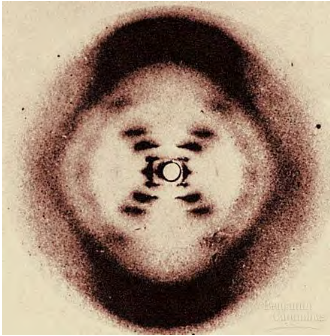
\includegraphics[width=0.5\linewidth]{./Figures/RF.png}
    \caption[Fotografía cristalográfica del ADN]{Fotografiá cristalográfica del ADN tomada por Rosalind Franklin en 1952}
    \label{fig:rf}
\end{figure}
El ultimo paso hacia la estructura del ADN fue llevado acabo por James Watson y Francis Crick en el laboratorio de Cavendish en francia, juntos trabajaron en diferentes modelos de la molécula de ADN , en 1953 publicaron un articulo en la prestigiosa revista Nature titulado: "molécular Structure of Nucleid Acids", el articulo solo tenia una pagina, pero era de un impacto significativo debido al modelo de ADN que contenía, un modelo de doble hélice(figura ~\ref{fig:jw}), ademas de esto, sugerían que el emparejamiento  especifico que habían postulado intuía un posible mecanismo para copiar material genético.
\begin{figure}[htbp]
    \centering
    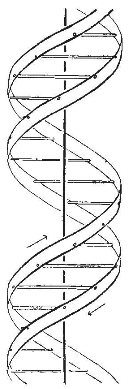
\includegraphics[width=0.15\linewidth]{./Figures/DNA1.png}
    \caption[Diagrama esquemático del ADN]{Diagrama esquemático del ADN publicado por Watson y Crick en 1953, imagen tomada de \cite{jwfc}.}
    \label{fig:jw}
\end{figure}
\subsection{Estructura del ADN}
el ADN es una molécula compuesta por dos largas cadenas, estas cadenas están formadas de múltiples
nucleótidos y cada
nucleótido esta compuesto por una base una molécula azúcar y un grupo fosfato.\\
El código genético del ADN esta representado por grupos de cuatro tipos de base con secuencias especificas. En el ADN, el azúcar es desoxirribosa, y esta unida a un grupo fosfato,  la base puede ser adenina (A), citosina (C), guanina (G), o timina (T), los nucleótidos están unidos covalentemente en una cadena mediante azúcar y fosfatos, y forman una estructura en forma de cadena alternando azúcar-fosfato-azúcar-fosfato. La estructura tridimensional del DNA(Doble hélice) surge de las características químicas y estructurales de las dos cadenas de
nucleótidos. Debido a que las dos cadenas se sostienen juntar debido a los enlaces de hidrógenos entre las base (A y T; G y C), todas las bases se encuentran en el lado interna de las hélices mientas que los grupos azúcar fosfato en la parte exterior\cite{rescells}.

\subsubsection{Daño inducido por radiación al ADN}

 Cualquier forma de radiación tiene el potencial de interactuar con estructuras claves como lo son los átomos para generar ionización, una vez suceda esto se inician eventos en cadena que llevan a cambios biológicos, estos efectos biológicos presentes en algún ser vivo debido a la radiación son relacionados a daños en el ADN.\\
 Esto se conoce como  acción directa de la radiación, y es el proceso dominante para radiación con gran cantidad de transferencia lineal de energía (LET) tales como partículas $\alpha$ o neutrones\cite{rescells}.\\

Por otro lado se tiene la acción indirecta de la radiación, este tipo de daño se ha demostrado mediante múltiples investigaciones\cite{willmari}, la radiación puede interactuar con los átomos de moléculas de una célula(particularmente con agua) para producir radicales libres, los cuales se pueden difundir lo suficientemente lejos para interactuar con objetivos críticos y causar daños, los radicales libres tienen electrones desapareados lo que causa gran reactividad química. La mayoría de la energía  depositada en células es inicialmente absorbida por el componente principal de las células, el agua, esto conlleva a una producción rápida de oxidantes y reductores de radicales hidroxilo reactivos. Los radicales hidroxilo pueden difundirse lo suficiente para interactuar con el ADN y causar daños. Afortunadamente, algunos sistemas defensivos o respuestas en las células pueden proteger a las células de los daños\cite{rescells}.\\

Evidencia acumulada en estudios radiológicos \cite{Franklin},\cite{rescells},  sugieren al ADN como el  objetivo sensible a la radiación. Esto se traduce en lesiones o modificaciones a genes y cromosomas, entender estos cambios son fundamentales para investigar y comprender la carcinogénesis, la muerte celular inducida por la radiación, y la transformación celular.\\


\paragraph{Rompimientos simples}
Un rompimiento simple es un rompimiento en un enlace peptídico, es decir azúcar fosfato, este daño es usualmente fácil de reparar, y en experimentos  se ha demostrado que aproximadamente el 90\% de los rompimientos simples son reparados en el curso de una hora a una temperatura de $37^{\circ} C$ \cite{Thormod}

\paragraph{Rompimientos dobles}

Este tipo de daño involucra las dos cadenas  del ADN, Si el enlace peptídico se rompe a cada lado dentro de una distancia de unos cuantos pares base se presentara un rompimiento doble, estos suelen estar relacionados con muerte celular y daño a los cromosomas.\\
Los rompimientos dobles son posibles de reparar, sin embargo, es mucho más difícil de reparar que un rompimiento simple,
la molécula de ADN contiene proteínas que suportan la estructura y previene que las piezas se caigan incluso cuando un rompimiento ocurre en ambas cadenas del ADN, de hecho, existen un numero de mecanismos que organismos complejos(como los humanos) han evolucionado para reparar los rompimientos dobles\cite{Thormod}.

\begin{figure}[htbp]
    \centering
    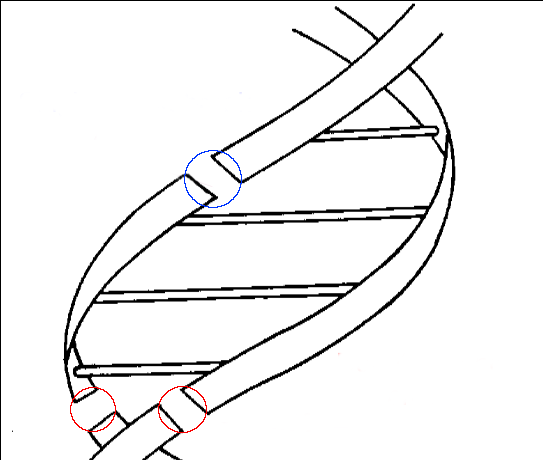
\includegraphics[width=0.5\linewidth]{./Figures/esbdb.png}
    \caption[Esquema rompimientos simples y dobles]{Rompimiento doble en rojo y rompimiento simple en azul, adaptada de \cite{Thormod}}
    \label{fig:esbdb}
\end{figure}


\paragraph{Daño base}

Como resultado de un fallo al reparar o de una falta de reparación, el codon(una secuencia de tres nucleótidos) alterado puede insertar un aminoácido incorrecto en la proteína y a su vez, la proteína modificada podría no funcionar correctamente, Si una base es alterada, la información puede cambiar o perderse,es conveniente mencionar que el daño a la base es uno de los puntos iniciales para la mutación. \\
Experimentos indican que la sensibilidad a la radiación varia de una base a otra. Después de una ionización inicial, rápidas organizaciones electrónicas toman lugar con el resultado de que el daño es transportado a ciertas regiones de la macromolécula (La guanina es particularmente sensible)\cite{Thormod}.

\paragraph{Dimeridos de pirimidina}

Se conoce a dímeros de pirimidina cuando dos bases adyacentes, (T y T, para la figura ~\ref{fig:dbdi})en la misma cadena se han alterado (sea químicamente o por cualquier otro motivo),  sucede entonces  que se necesita una de las cadenas para replicar la cadena siguiente, como efecto cuando ambas cadenas están dañadas en el mismo sitio no hay manera de que esto se lleve acabo.

\begin{figure}[htbp]
    \centering
    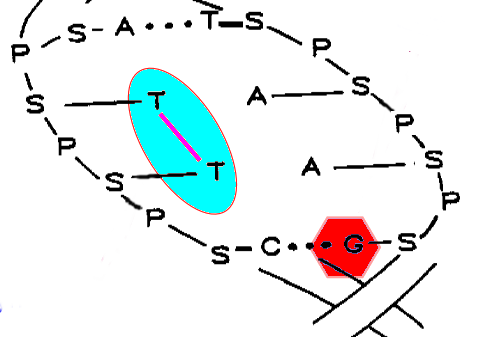
\includegraphics[width=0.5\linewidth]{./Figures/base-piri.png}
    \caption[Esquema Daño base y Dimeridos]{ Daño de la base en rojo y dímeros de pirimidina en cian, adaptada de \cite{Thormod}}
    \label{fig:dbdi}
\end{figure}

\subsection{Daño Celular}
Antes de seguir es importante aclarar porque es importante el daño ocasionado por radiación ionizante a las células. En general los organismos complejos como los animales y las plantas, están compuestos de células procariotas, estás células contienen la unidad molecular de información conocida como gen el cual se encargada de la herencia genética, o en otras palabras la transferencia de características de los individuos a su descendencia, esta información genética esta codificada por el ADN y es empacada en cromosomas, el conjunto de todos los genes de los cromosomas se conoce como genoma. Lo anterior es relevante debido a que el ADN es extremadamente importante en la replicación celular y un daño a este puede ocasionar aberraciones de cromosomas y mutación de genes, lo que genera subsecuentes efectos biológicos.\\
\\
A su vez también es notable mencionar que la irradiación puede afectar células malignas afectando la estructura, estabilidad, y reparación del ADN, invocando procesos como rompimientos dobles y induciendo efectos terapéuticos contra las células tumorales tales como apoptosis, necrosis,  senescencia, y mitosis anormal como se menciona en \cite{cancer}.\\


%La radiación ionizante se encuentra en nuestro ambiente natural y %también es generada y usada por la humanidad, usos médicos. Un %entendimiento mejor de los efectos biológicos de la radiación %ionizante lleva a un uso y una protección mejor de la radiación. %La respuesta de las células a la radiación sera descrita y %discutida. La significancia de la consecuencias de varios tipos de %radiación inducida-daño de ADN, muestra que el ADN es el principal %blanco para efectos biológicos de la radiación. los daños %reparados mal o que no se reparan, en particularmente en el ADN %los rompimientos dobles, induciran aberraciones de cromosonas y %mutacipon de genes, en la otra mano, la radiación-inducida %rompimientos dobles en el ADN juega un rol importante en la %inducción de apoptosis y punto de control del ciclo celular

\subsubsection{Reparación del ADN}

Las encimas se encargan de la reparación en las células, dependiendo de su función algunas encimas se encargan de ubicar el daño en el ADN mientras que otras son llamadas a reparar el daño, según \cite{Thormod} los procesos de reparación pueden ser divididos en tres tipos:
\begin{enumerate}
\item Las encimas trabajan directamente en el sitio dañado. La secuencia original de la base se conserva.
\item Todo el tramo de ADN que contiene un sitio (o sitios) dañados se eliminan y se reemplazan, preservando la secuencia original.
\item El daño se ignora durante la replicación, se pasa por alto, si se tiene suerte se insertará la base correcta, si es incorrecta no importará. Debido a que este tipo de reparación es propenso a errores, se mantiene en reserva en caso de que los sistemas de reparación de mayor fidelidad pierdan o no puedan hacer frente al daño. Por esta razón, se le conoce como reparación "SOS".
\end{enumerate}


\paragraph{Reparación por escisión}
Un mecanismo importante es encontrado en humanos y microorganismos es la "Reparación por escisión" , este mecanismo envuelve enzimas que cortan la parte dañada del ADN y lo reemplaza con una nueva parte sin daño alguno\cite{Thormod}.
\begin{enumerate}
  \item Las encimas se encargan de buscar y encontrar los sectores dañados, si encuentran un sector dañado enviaran una señal de ayuda.

  \item Ciertas encimas especificas se encargarán de cortar la proximidad donde se encuentra el daño al ADN.

  \item La enzima exonucleasa se encarga de cortar la parte dañada del ADN por completo y luego la polimerasa reemplazara con una parte completamente nueva sin daño alguno.

  \item Por ultimo una enzima conocida como ligasa se encargara de unir esta nueva parte con el resto de la cadena de ADN, de esta forma el ADN vuelve a su estado original.
\end{enumerate}


\paragraph{Reparación de rompimientos dobles}

La protección del genoma requiere la capacidad de reparar rompimientos dobles y para asegurar que la reparación es llevada acabo con suficiente fidelidad, existen dos caminos principales para reparaciones de rompimientos dobles, llamados recombinación homologa, y recombinación no homóloga, la primera libre de errores y la segunda propensa a errores \cite{rescells}.

\subparagraph{Recombinación homologa}
Este es un mecanismo de alta fidelidad y eficiente para reparar rompimientos dobles en el ADN, recupera la información perdida en el sitio del rompimiento de la cromátida hermana no dañada o del cromosoma homólogo, en el curso de la recombinación homologa, el ADN dañado contacta físicamente al DNA indemne con una secuencia homologa, luego usa esto como una plantilla para reparar\cite{rescells}.

\subparagraph{Recombinación no homologa}

La reparación no homologa del ADN  es un proceso que se basa en volver unir los dos extremos de un rompimiento doble sin el requisito de homología de secuencia entre los dos extremos. El proceso puede describirse como una serie de pasos que pueden ser consultados en \cite{rescells}.
%lo pasos son los siguientes:

%Paso inicial: unión de un complejo heterodimérico para el ADN dañado. El complejo consta de las proteínas Ku70 y Ku80 (también conocido como XRCC5). La unión del complejo protegerá el ADN de la digestión de exonucleasa. En la unión, Ku80 es distante  mientras que Ku70 es próxima a la ruptura del ADN.

%Formación de ADN-PKcs. Después de la unión, el heterodímero Ku se asocia con la subunidad catalítica de DNA-PK (XRCC7, DNA-PKcs) para formar la holoenzima de DNA-PK activa. DNA-PKcs se activa mediante la interacción con un DNA de cadena sencilla en el sitio del rompimiento doble y muestra actividad Serina/treonina quinasa

%Enlace de dos extremos. XRCC4 forma un complejo estable con ADN ligasa IV, y este complejo se une a los extremos de las moléculas de ADN y une moléculas de ADN dúplex con extremos complementarios pero no ligables. El complejo XRCC4 - ligasa IV no puede volver a ligar directamente la mayoría de los rompimientos dobles generados por agentes inductores de rompimientos dobles.

%Eliminación de factores relacionados con recombinación no homologa. Los factores relacionados con recombinación no homologa deben eliminarse del ADN antes de reparar los rompimientos dobles. La auto-fosforilación de DNA-PKcs y/o DNA-PK mediante la fosforilación de factores accesorios son importantes en la liberación de DNA-PKcs y Ku del rompimiento doble antes de la unión final. Finalmente, la reparación se completa, aunque los nucleótidos a menudo se pierden, lo que resulta en una reparación inexacta.


\subsubsection{Mecanismos de defensa}
\paragraph{Contra las especies reactivas de oxígeno}
El daño al ADN puede ser causado en general por dos tipos de procesos:\\
 \textbf{endógenos(interior)}:son causado principalmente por radicales reactivos de oxígeno.\\
 \textbf{exógenos(exterior)}: debido a diferentes fuentes como radiación ionizante, rayos UV y sustancias químicas.\\
Las especies reactivas de oxígeno  son producidas por el metabolismo del oxígeno. La mayor parte molecular del oxigeno se convierte en $CO2$.\\
mientras que una pequeña fracción (aproximadamente 5 \%) se convierte en especies reactivas de oxígeno. Las enzimas y los eliminadores de radicales libres se ocupan principalmente de esta producción endógena. Sin embargo, se produce algún daño en el ADN, proteínas, lípidos y carbohidratos\cite{Thormod}.

\paragraph{Un grupo de células dañadas por ADN}

El número de daños en el ADN de los mecanismos endógenos y exógenos es muy grande, y debido a esto se tiene un grupo de células dañadas. Mientras estas células esten en la fase de reposo G0 en la mitosis celular la situación está bajo control. Sin embargo, Cuando las células dañadas entran en el ciclo celular se da el paso inicial en el desarrollo del cáncer, una célula dañada que se promueve en el ciclo celular. En consecuencia. Las rutas principales para tratar con este problema son:\\
Mecanismos de reparación: Estos ya se han mencionado anteriormente en el documento.\\
Muerte celular: La otra posibilidad es matar la célula dañada, las células tienen un mecanismo llamado "apoptosis" o "muerte celular programada" que puede activarse con el resultado de que la célula dañada se destruya mientras que el organismo sobrevive\cite{Thormod}.

\paragraph{Puntos de control en el ciclo celular}

En el ciclo celular se encuentran varios puntos de control a través del ciclo. Si en algún momento se presenta daño en el ADN, el ciclo celular se detiene y se da tiempo para reparar. Si la reparación no tiene resultados substanciales, puede desencadenarse la muerte celular, como la apoptosis.


\subsubsection{Respuesta adaptativa}
Se conoce como respuesta adaptativa al fenómeno que se presenta cuando se aumenta la resistencia a la radiación de una  célula viva con pequeñas dosis de radiación.
Los experimentos que exhiben una respuesta adaptativa comenzaron en 1984 con el trabajo sobre linfocitos humanos por G. Olivieri, J. Bodycote y S. Wolff en la Universidad de California. Con experimentos donde irradiaban las células con partículas $B$ de tritio y rayos X, después se guardaban  las aberraciones a los cromosomas para ser analizadas. Se descubrió que el número de aberraciones era menor después de la exposición a ambas fuentes (partículas B de tritio y rayos X) en comparación a después de  solo los rayos X. Estos resultados mostraron que los bajos niveles de radiación pueden desencadenar o inducir una mayor reparación de roturas cromosómicas inducidas por la radiación.
A lo largo de la década de 1990, se publicaron una gran cantidad de experimentos en diferentes sistemas que demuestran una respuesta adaptativa. Se han estudiado varios puntos finales, tales como destrucción celular, formación de micronúcleos, inducción de aberraciones cromosómicas, inducción de mutaciones y transformaciones neoplásicas\cite{Thormod}.


% SEC3

\clearpage

\section{Interacción radiación-materia}
\label{sec:Intro}
En general este apartado se basa en dar una pequeña explicación de algunos fenómenos físicos relevantes en la interacción radiación materia, estos se basan en las diversas interacciones de partículas cargadas o fotones con átomos, existen otros procesos que son relevantes como la interacción de neutrones pero debido a que poco tienen que ver(por ahora) con el desarrollo de este trabajo no son incluidos.
\subsection{Interacciones de fotones en la materia}
 A menudo se asume que son solo cuatro los eventos relevantes para fotones al interactuar con átomos: dispersión de Compton, dispersión de Rayleigh, efecto fotoelectrico, y producción de pares.
Pero en Realidad las interacciones más importantes de fotones con la matería son principalmente seis, las cuales son: dispersión de Compton, dispersión de Rayleigh, efecto fotoelectrico, producción de nuclear de pares, producción electrónica de pares, y reacciones fotonucleares, esto es debido a que usualmente la producción de nuclear de pares junto a la producción electrónica de pares se manejan ambas bajo el nombre de producción de pares y los efectos de las reacciones fotonucleares son ignorados. A continuación se muestra una explicación sencilla de cada uno de ellos.

\paragraph{Dispersión de Compton(Dispersión incoherente)}

El efecto Compton recibe su nombre en honor a Arthur Compton quien en 1922 fue la primer persona en realizar mediciones de una dispersión entre un fotón y un electrón libre, este fenómeno se basa en la interacción de un fotón con una energía $h\nu$ junto con un electrón débilmente ligado a un orbital de cierto átomo, cuando esto ocurre, se produce un fotón de energía menor $h\nu '$ y un electrón conocido como el electrón de Compton(dispersado) es expulsado del átomo con una energía cinética $E_k$, es pertinente mencionar que en estudios teóricos se asume que el electrón esta libre y estacionario\cite{Podgorsak}, generalmente es posible usar los cálculos de mecánica clásica con la conservación de energía y momento, sin embargo es importante entender la naturaleza cuántica del proceso, y en particular la transferencia de energía y la asignación de momento a un fotón implicada, los cálculos clásicos funcionan mientras, la velocidad no sea relativista, la energía de los fotones implicados no sea muy baja o el material tenga un numero atómico $Z$ muy alto, si alguna de estas situaciones se cumple es necesario realizar las correcciones apropiadas\cite{Edward}.\\
\begin{figure}[htbp]
    \centering
    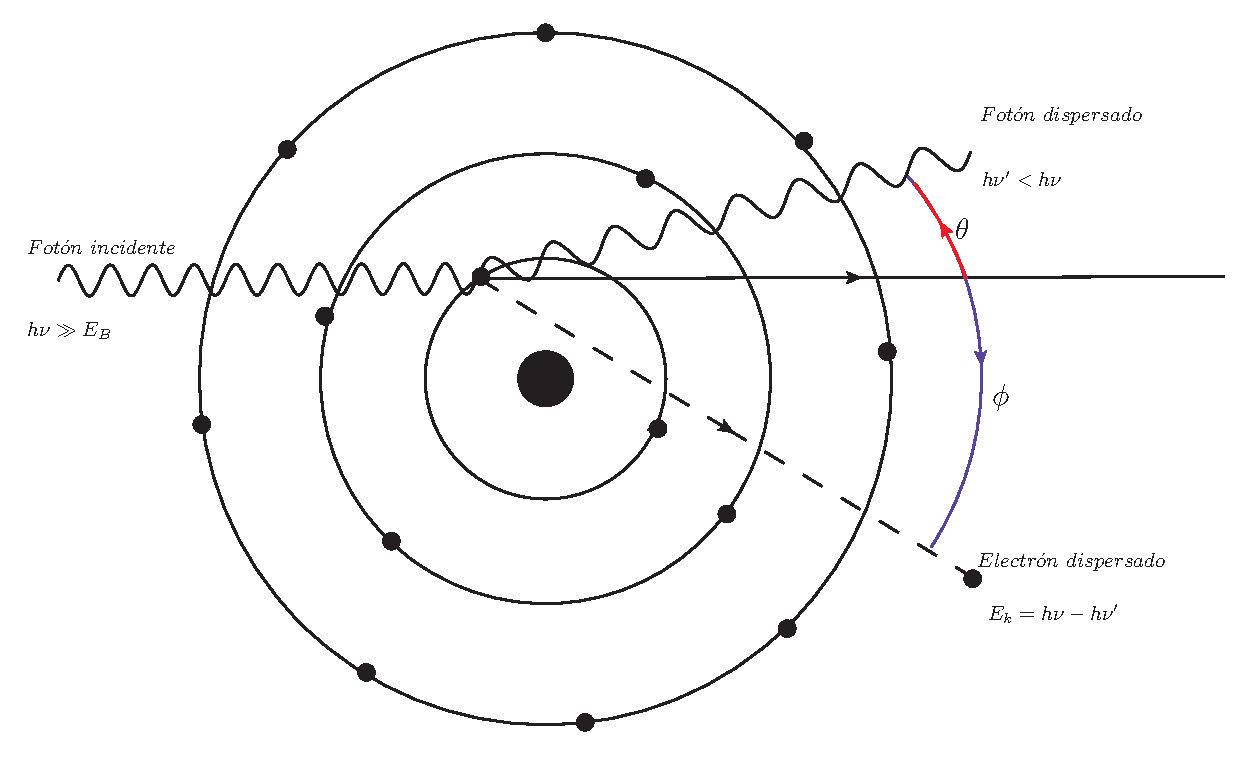
\includegraphics[width=.71\linewidth]{./Figures/compton1.eps}
    \caption[Efecto Compton]{Efecto Compton: un fotón incidente con energía $h\nu$ colisiona con un electrón débilmente ligado de un átomo produciendo un fotón con energía menor $h\nu '$ con angulo $\theta$ y a su vez es expulsando un electrón de Compton con energía cinética $E_k$ y angulo $\phi$}
    \label{fig:Compton}
\end{figure}

\paragraph{Dispersión de Rayleigh(Dispersión coherente)}
Recibe el nombre de Rayleigh debido a el físico John W. Rayleigh quien en 1900 desarrollo una teoría para la dispersión de radiación electromagnética debido a átomos, este fenómeno ocurre principalmente con fotones a bajas energías $h\nu$ junto con un receptor que tenga numero atómico $Z$ alto, consiste en que un fotón incidente es dispersado cuando interactuá con alguno de los electrones ligados a un átomo, el átomo absorbe el momento transferido y el fotón es dispersado con un angulo $\phi$ y con una energía relativamente igual a la que tenía antes de la interacción, los ángulos de este fenómeno son relativamente pequeños dado que la energía impartida al átomo no produce ionización o excitación y este vuelve a su estado original después de la interacción\cite{Podgorsak}.
Tambíen se conoce como Dispersión coherente debido a que el fotón es dispersado por  la acción combinada de todo el átomo,debido a esto el evento es elástico en el sentido de que el fotón no pierde casi nada de su energía\cite{Frank}.

\begin{figure}[htbp]
    \centering
    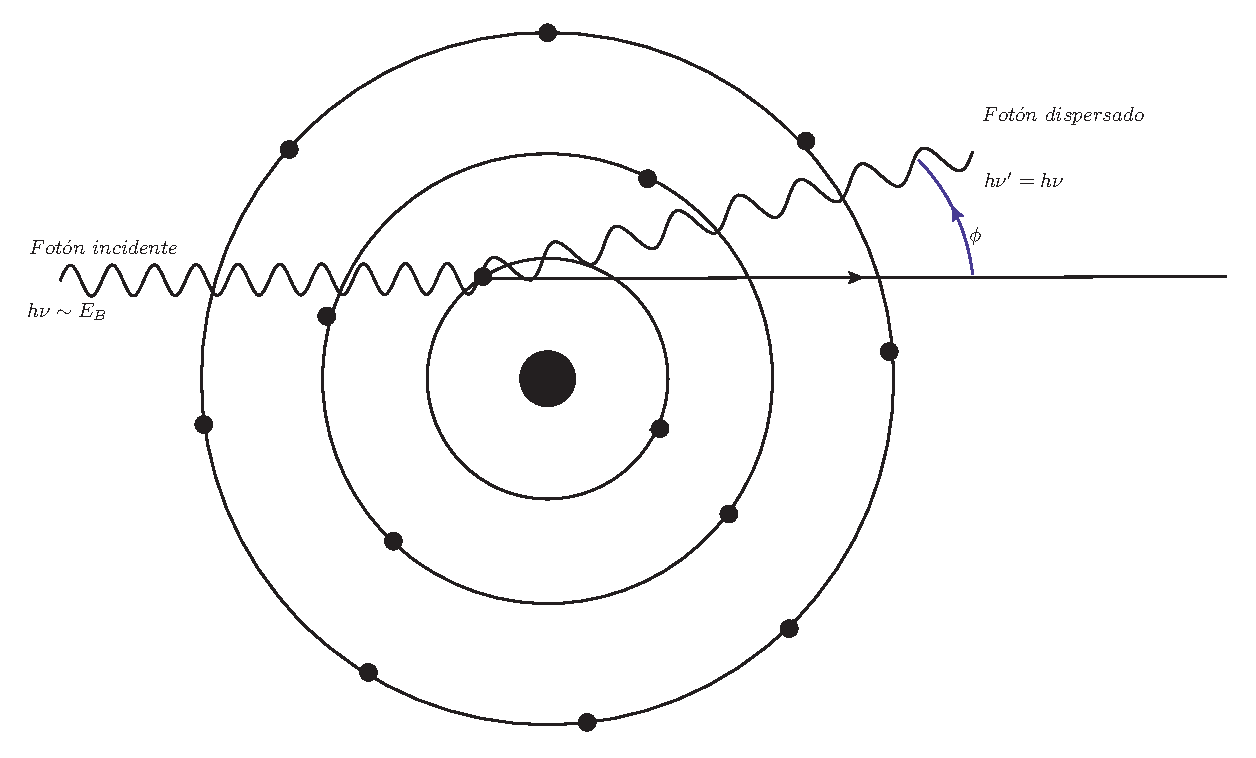
\includegraphics[width=.71\linewidth]{./Figures/Ray.eps}
    \caption[Dispersión de Rayleigh]{Dispersión de Rayleigh:un fotón incidente con energía $h\nu$ interactuá con un electrón ligado a un átomo, este fotón es dispersado con un angulo pequeño $\phi$ y una energía $h\nu '$ relativamente igual a $h\nu$ }
    \label{fig:UoC}
\end{figure}


\paragraph{Efecto Fotoelectrico}

Se conoce como efecto fotoeléctrico a la interacción entre un fotón y un electrón orbital fuertemente ligado a un átomo, el fotón incidente con energía $h\nu$ interactúa con el electrón del átomo, entonces es absorbido completamente y el electrón orbital conocido como fotoelectrón es expulsado con energía cinética $E_k=h\nu-E_B(K)$ Donde $E_B(K)$ es la energía de ionización del electrón, la vacante en el orbital es subsecuentemente tomada por con un electrón más alto y la energía de la transición del electrón sera emitida en la formá de un fotón característico(fluorescencia) o como un electrón de Auger.

A diferencia del efecto Compton el cual ocurre cuando un fotón interactuá con un electrón "libre"(débilmente ligado), el efecto fotoeléctrico sucede entre un fotón y un electrón "ligado fuertemente", la diferencia entre estos radica en la magnitud relativa de la energía del fotón $h\nu$ y la energía necesaria para remover un electrón de un átomo(energía de ionización) $E_B$ en vez de un valor absoluto de $h\nu$ o $E_B$, entonces cuando $E_B\ll h\nu$ se dice que el electrón esta débilmente ligado o libre y cuando  $E_B \lesssim h\nu$ se asume que el electrón esta fuertemente ligado\cite{Podgorsak}.


\begin{figure}[htbp]
    \centering
    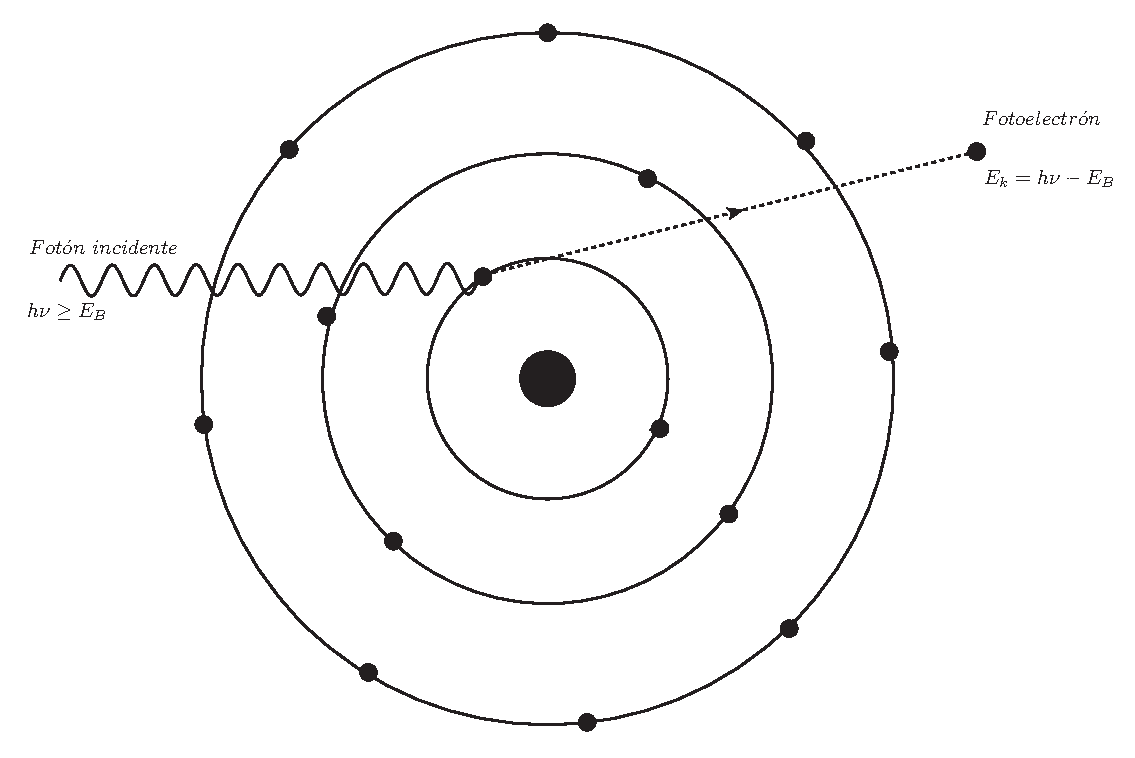
\includegraphics[width=.71\linewidth]{./Figures/fotoelec.eps}
    \caption[Efecto fotoeléctrico]{Efecto fotoeléctrico: un fotón incidente con energía $h\nu$ interactúa con el electrón del átomo, entonces es absorbido completamente y el electrón orbital conocido como fotoelectrón es expulsado con energía cinética $E_k$}
    \label{fig:UoC}
\end{figure}

\paragraph{Producción de pares}
Si un fotón con una energía mayor  1.02 MeV entra en un receptor, puede interactuar con los átomos de este por un proceso conocido como producción de pares, en este mecanismo de transferencia de energía el fotón al pasar cerca del átomo esta sujeto a efectos de campo fuerte debido al núcleo, y puede desaparecer y reaparecer como un par de electrones positivo y negativo.\cite{Edward}
Debido a que el momento $p_\nu$ antes de la interacción de producción de pares es mucho más grande que el momento total  $p_{pair}$ después de la interacción de producción de pares,  entonces el fotón debe poseer un exceso de momento que no puede ser absorbido por el par electrón-positrón, por tanto, debe ser absorbido por otro ente de colisión, sea el núcleo atómico, o un electrón orbital\cite{Podgorsak}, dada alguna de estas condiciones tenemos:
\subparagraph{Producción nuclear de pares}
 Cuando el fotón interactuá con el núcleo atómico, esté juega un rol más o menos pasivo, el estado del núcleo dispersado antes y después del evento es el mismo, excepto por un cambió en su energía cinética y momento. Simplemente un fotón se ha convertido en un electrón y un positrón\cite{Edward}.
\begin{figure}[htbp]
    \centering
    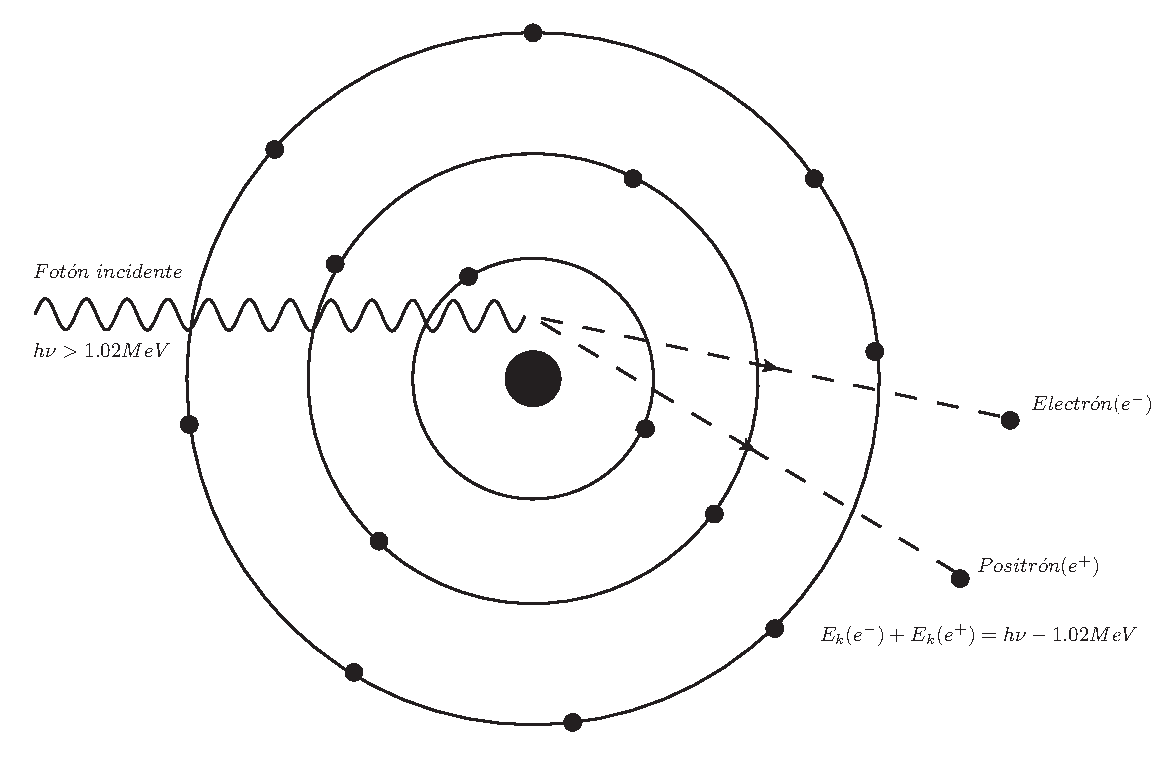
\includegraphics[width=.71\linewidth]{./Figures/nuclearpp.eps}
    \caption[Producción nuclear de pares]{Producción nuclear de pares: Un fotón experimenta una producción de pares estándar, electrón--Positrón}
    \label{fig:UoC}
\end{figure}
\subparagraph{Producción electrónica de pares}
 El fotón incidente interactúa con un electrón orbital, en lugar de con un núcleo atómico, debido a esto el electrón es dispersado, dado que tiene una masa pequeña, tomará una energía cinética significativa y aparecerá como un producto de la interacción. Además, un electrón y un positrón se generan como resultado de la desaparición del fotón incidente \cite{Edward}.
\begin{figure}[htbp]
    \centering
    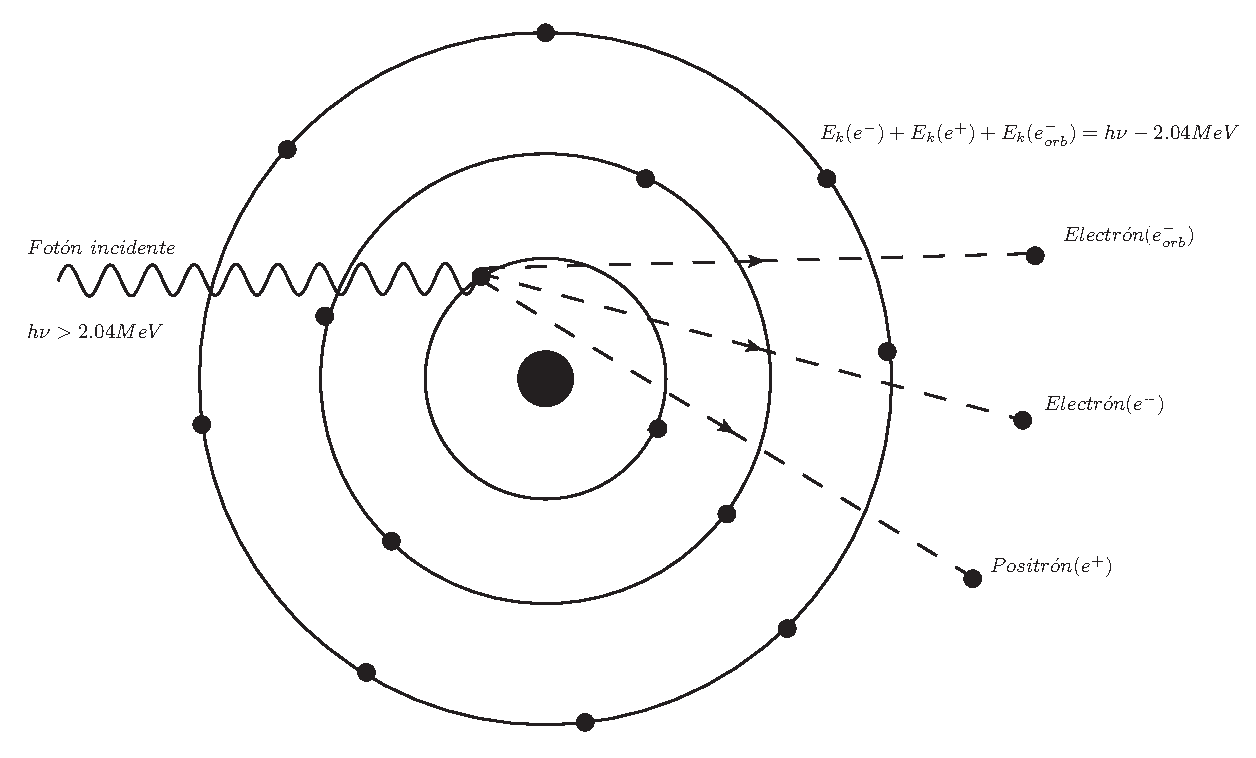
\includegraphics[width=.71\linewidth]{./Figures/electpp.eps}
    \caption[Producción electrónica de pares]{Producción electrónica de pares: Un fotón experimenta una producción de pares triple, un electrón dispersado--electrón--Positrón}
    \label{fig:UoC}
\end{figure}

\paragraph{Reacciones fotonucleares}
 Usualmente este tipo de fenómeno también recibe el nombre de "fotodesintegración" ó "efecto nuclear fotoeléctrico", se basa en la interacción entre un fotón energético y un núcleo causando desintegración nuclear. En la reacción fotonuclear el núcleo absorbe el fotón y el resultado más probable es la emisión de un solo neutrón, aunque es posible que se emitan otras partículas como $\alpha$, rayos $\gamma$,más de un neutrón o fragmentos de fisión, aunque estos eventos son menos probables, un neutrón producido por este fenómeno se conoce como fotoneutrón\cite{Podgorsak}.

 \begin{figure}[htbp]
     \centering
     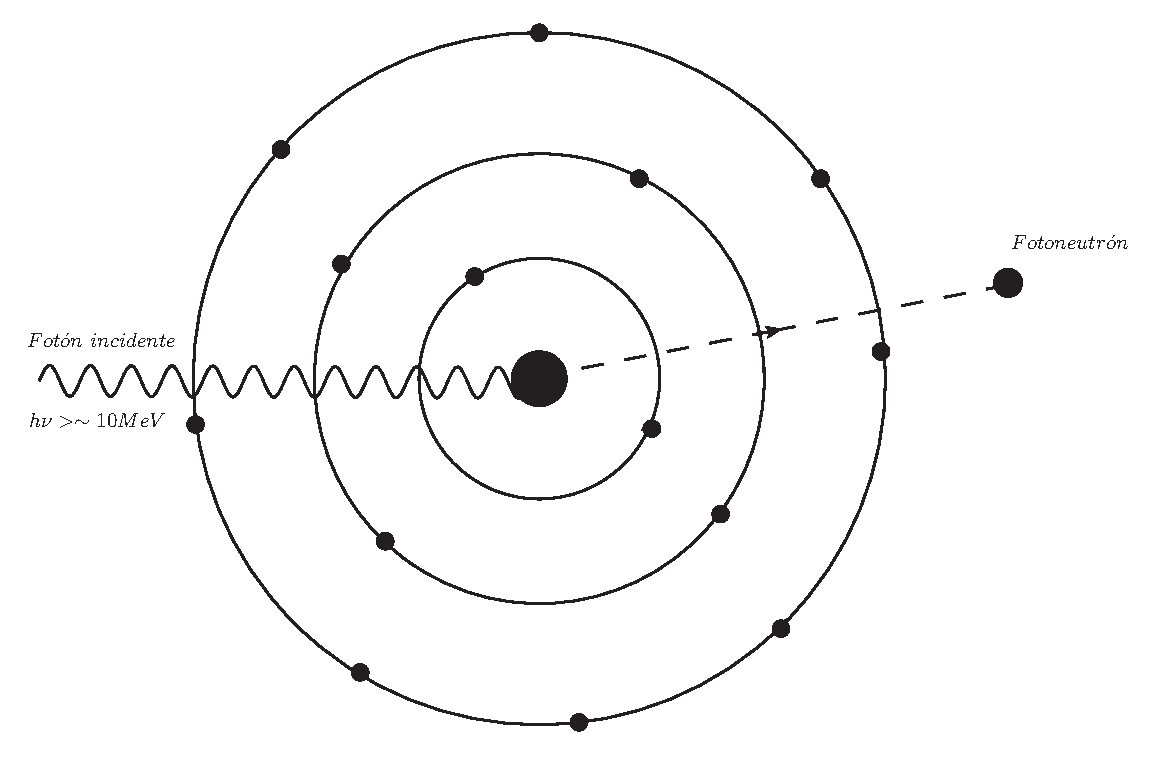
\includegraphics[width=.71\linewidth]{./Figures/fotoneu.eps}
     \caption[Reacción fotonuclear]{Reacción fotonuclear: Un fotón es absorbido por un núcleo atómico y esté produce un fotoneutrón}
     \label{fig:UoC}
 \end{figure}


\subsection{Interacciones de partículas cargadas en la materia}
A medida que una partícula viaja en un receptor experimenta interacciones de Coulomb con los núcleos y electrones de los átomos de este mismo, estas interacciones pueden ser divididas en tres categorías dependiendo del tamaño clásico del parámetro de impacto $b$ de la trayectoria de la partícula cargada comparado al radio clásico del átomo $a$ con el que la partícula interactuá
\paragraph{Colisión de radiación($b\ll a$)}
Cuando el parámetro de impacto $b$ de una partícula cargada es mucho más pequeño que el radio $a$ del átomo, la partícula cargada interactuá más que todo con el núcleo y experimenta dispersión elástica o inelástica junto con un posible cambio en la dirección del movimiento. En la mayoría de los casos se presenta dispersión elástica en cuyo caso la partícula es dispersada por el núcleo pero solo sufre una pequeña perdida de su energía cinética, sin embargo un pequeño porcentaje de estas interacciones son inelasticas y pueden resultar en perdida significante de energía para la partícula cargada acompañada por la emisión de fotones de rayos-x, este tipo de interacción se conoce como colisión de bremsstrahlung\cite{Podgorsak}.


\subparagraph{Bremsstrahlung}
Bremsstrahlung es un tipo de fotón de rayos-x producido cuando partículas ligeras experimentan interacción radioactiva inelástica con núcleos de átomos de dado receptor, en esta interacción la partícula presenta ralentización
 dando una fracción significante de energía cinética al fotón\cite{Frank}. Las partículas cargadas de interés para la física medica y dosimetría se pueden clasificar en dos categorías:

1. Partículas ligeras cargadas: electrones $e-$ y positrones $e+$, ambos pueden producir fotones bremsstrahlung debido a su masa relativamente pequeña\cite{Podgorsak}.\\
2. Partículas pesadas cargadas: protones $p$, deuterones $d$, partículas alfa $\alpha$, iones pesados tales como $Li^+$,$Be^+$,$C+$,$Ne+$, etc. producen una cantidad insignificante de fotones bremsstrahlung\cite{Podgorsak}.

Bremsstrahlung es la palabra en alemán para designar radiación de frenado.

\begin{figure}[htbp]
   \centering
   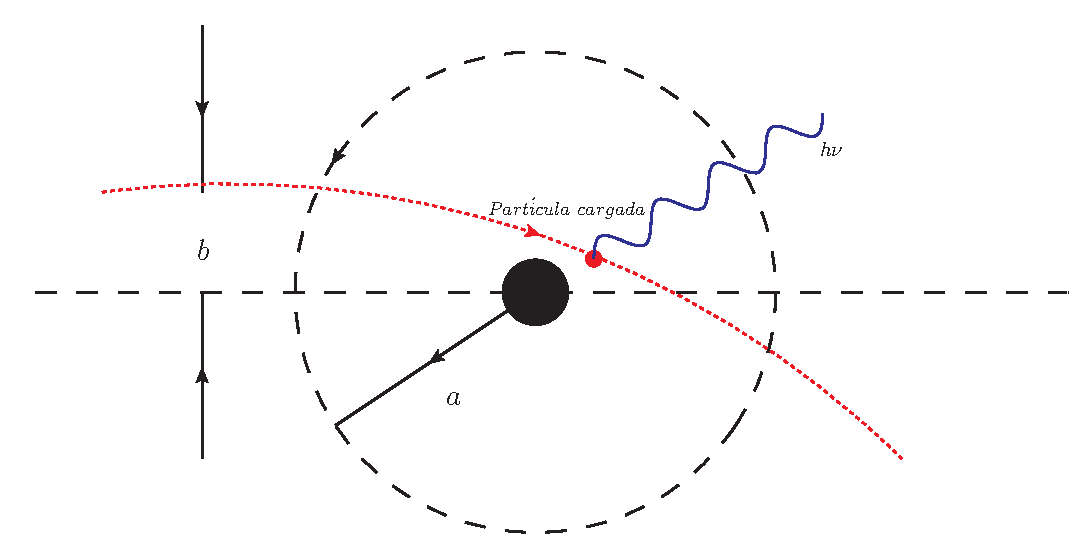
\includegraphics[width=.65\linewidth]{./Figures/radiacol.eps}
   \caption[Colisión de radiación]{Colisión de radiación(producción de bremsstrahlung)}
   \label{fig:UoC}
\end{figure}


\paragraph{Colisión fuerte($b\approx a$)}
Cuando el parámetro $b$ de la trayectoria de una partícula cargada sea aproximadamente del orden del radio $a$ del átomo,la partícula cargada puede tener un impacto directo de Coulomb con un electrón de un orbital, a este fenómeno se le conoce como Colisión fuerte en el cual se transfiere una cantidad significante de energía de la partícula al electrón, luego de la interacción el electrón deja el átomo como un rayo $\gamma$, el numero de colisiones fuertes que  experimenta  una partícula cargada moviéndose en un receptor es generalmente pequeño, sin embargo la transferencia de energía asociada es relativamente grande\cite{Podgorsak}.


\begin{figure}[htbp]
   \centering
   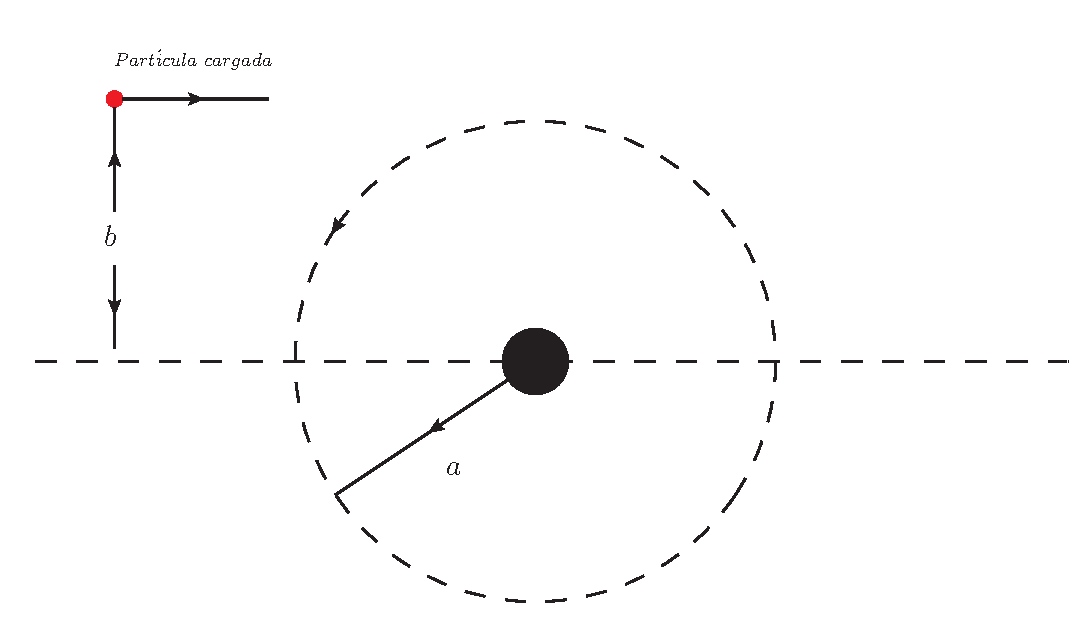
\includegraphics[width=.65\linewidth]{./Figures/hardcoli.eps}
   \caption{Colisión fuerte}
   \label{fig:UoC}
\end{figure}

\paragraph{Colisión debil($b\gg a$)}
Cando el parámetro $b$ de la partícula cargada es mucho más grande que el radio $a$ del átomo, la partícula cargada interactuá con todo el átomo el cual se compone de electrones ligados, la energía transferida por la partícula cargada en este evento a los electrones ligados es muy pequeña, sin embargo el numero de estas interacciones es bastante grande, y debido a esto la partícula pierde mucha energía, estas mini-interacciones pueden causar polarización atómica, excitación o ionización mediante la remoción de un electrón de valencia, este fenómeno recibe el nombre de colisión débil o colisión suave\cite{Podgorsak}.

\begin{figure}[htbp]
   \centering
   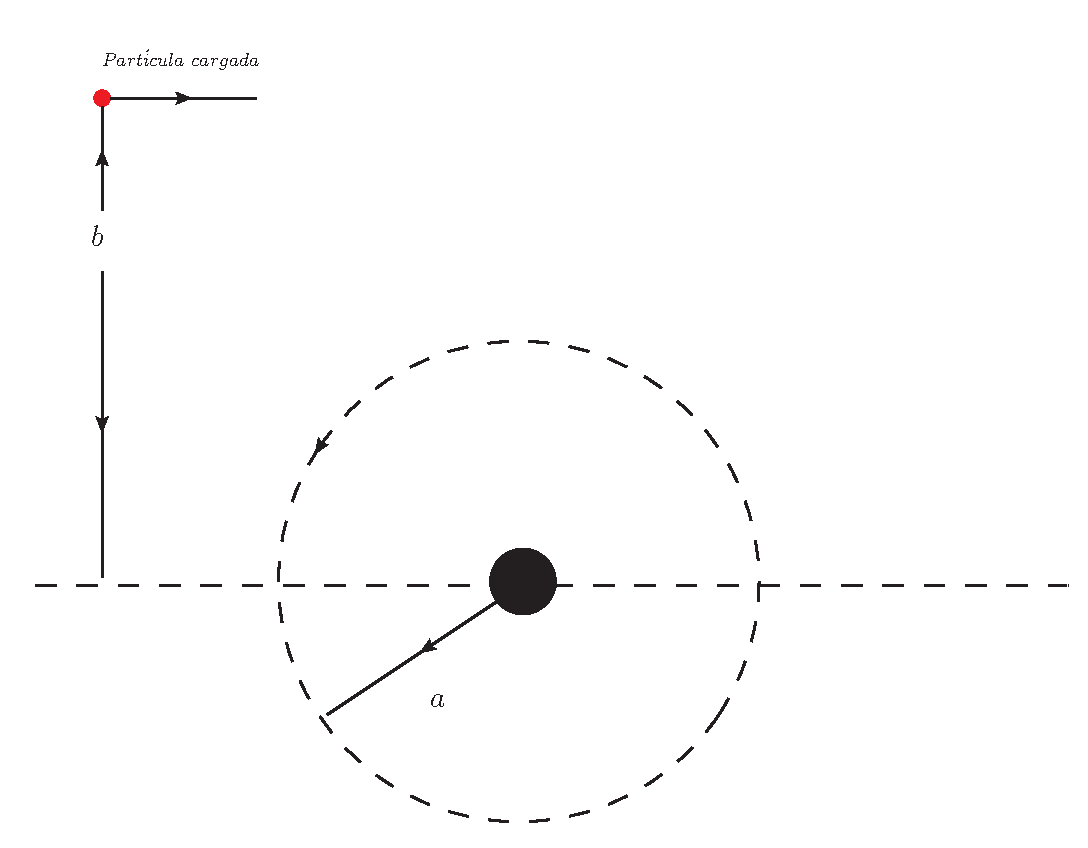
\includegraphics[width=.65\linewidth]{./Figures/softcoli.eps}
   \caption{Colisión débil o suave}
   \label{fig:UoC}
\end{figure}


% SEC4

\clearpage

\section{GEANT4}
\label{sec:GEANT4}
GEANT4(\textbf{GE}ometry \textbf{AN}d \textbf{T}racking - \textbf{4} versión) es una plataforma computacional para la simulación de diversos procesos físicos que se centra en la interacción de partículas viajando a través de la materia haciendo uso de Montecarlo. Geant es creado en 1974 por el CERN pensado originalmente para la simulación de experimentos en física de altas energías, esto cambiaría con el desarrollo de subsecuentes versiones las cuales serían empleadas en muchos otros campos, su cuarta versión Geant4 es publicada en 1998, esta última a su vez también ha tenido diversas versiones actualizadas cada año, su lanzamiento más reciente ha sido Geant4-10.5.p01 y su versión beta Geant4-10.6-beta ambas versiones liberadas en el presente año,  cuenta  con áreas de aplicación que incluyen física de altas energías, física espacial, física médica, transferencia tecnológica, entre otras, su desarrollo, aplicación y mantenimiento son debido al equipo colaborativo a nivel global Geant4 Colaboration los cuales se centran en que el software pueda ser lo mejor posible.
\\
\\
GEANT4 se proporciona bajo la licencia \href{https://geant4.web.cern.ch/license/LICENSE.html}{\color{blue}{Geant4 Software License}}.

\subsection{PDB4DNA}

PPB4DNA es una aplicación relativamente nueva de Geant4 creada por Geant4-DNA project, se basa en el uso adicional de una librería construida en c++ llamada PDBlib, la cual permite hacer uso de la estructura atómica de una molécula de ADN al extraer datos que se encuentran en un archivo .pdb para posteriormente ser usados en Geant4 para evaluar el daño inducido por partículas ionizantes al mismo, mediante un conteo de rompimientos simples, rompimientos dobles y su correspondiente deposición de energía.

El objetivo principal de Geant4-DNA project es extender Geant4 con diversos procesos para el modelar el daño biológico inducido por radiación ionizante en la escala del ADN, es coordinado desde el 2008 por el National Institute for Nuclear and Particle Physics (IN2P3) del National Centre for Scientific Research (CNRS) en Francia.


\subsubsection{PDB}
Un archivo .pdb (Protein Data Bank) es un archivo de texto que contiene la información estructural de una molécula, se compone de cientos a miles de líneas y en general debe contener lo siguiente\\
HEADER: Registra si la molécula es ADN o proteína.\\
REMARK: Designa comentarios los cuales pueden dar información relevante.\\
ATOM: Registra el símbolo del átomo, id de cadena, numero de residuo o nucleótido y coordenadas espaciales x y z. \\
Para observar un ejemplo de cómo está conformado un archivo pdb véase figura ~\ref{fig:pdbesq}.
\begin{figure}[htbp]
    \centering
    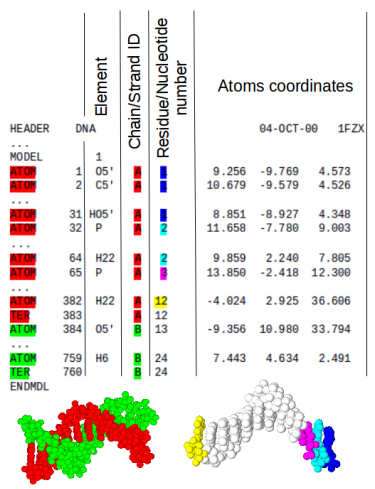
\includegraphics[width=.5\linewidth]{./Figures/pdb.png}
    \caption[Esquema de un PDB]{Esquema de un PDB, imagen tomada de\cite{pdblib}} % se puede realizar grafico en vmd}
    \label{fig:pdbesq}
\end{figure}

\subsubsection{pdb reader}
Está funcionalidad presente en PDBlib permite leer la estructura molecular de un pdb en Geant4 sin la necesidad de usar otras librerías de terceros, la función se encarga de recolectar la siguiente información: elemento, id de cadena, numero de residuo y coordenadas del átomo, mediante el uso de palabras clave como ATOM y TER\cite{pdblib}.
\subsubsection{Visualización}
Pdb4dna viene preestablecido con la molécula 1ZBB esto debido a que describe la estructura de ADN más grande que se encuentre en formato pdb, el ejemplo hace uso de la geometría de Geant4 simplemente para objetivos de visualización como formas, distribución espacial, materiales y atributos de visualización para cada átomo, por ahora PDB4DNA solo presenta tres modos de visualización, esferas ligadas(baricentros), vista atómica (VDW) y residuos\cite{pdblib}.

\begin{figure}[htbp]
    \centering
    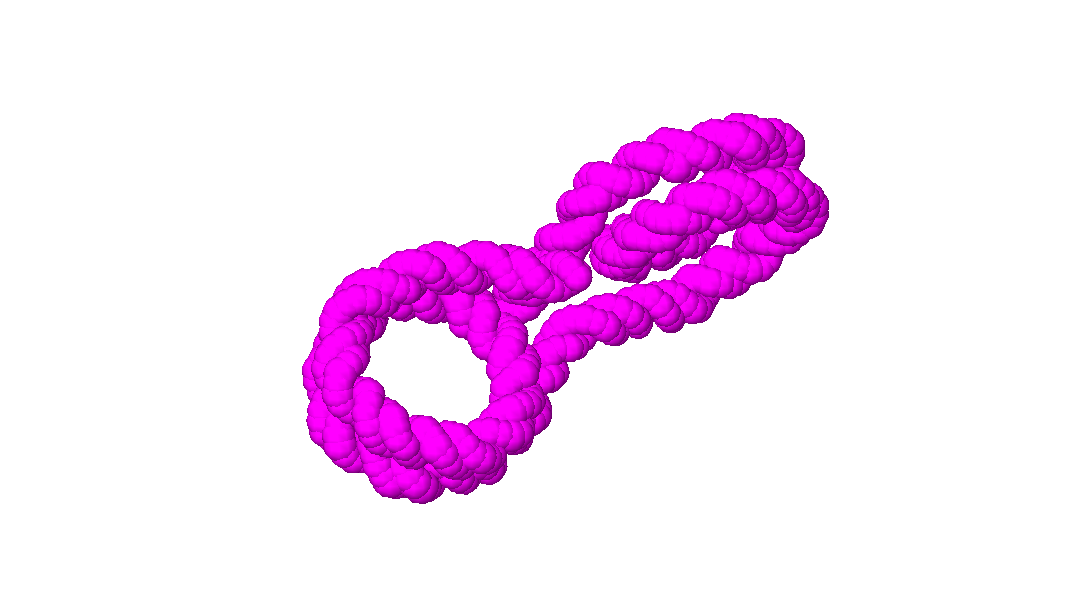
\includegraphics[width=.7\linewidth]{./Figures/ba.png}
    \caption{Barycentros}
    \label{fig:ba}
\end{figure}


\begin{figure}[htbp]
    \centering
    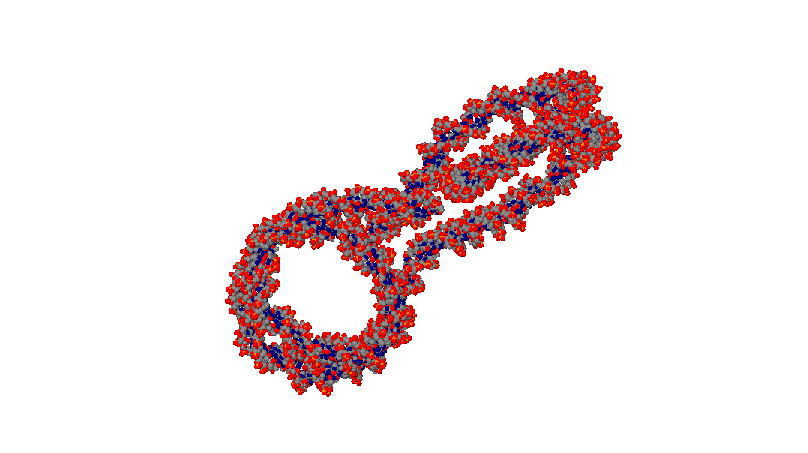
\includegraphics[width=.7\linewidth]{./Figures/cpk.png}
    \caption{VDW}
    \label{fig:cpk}
\end{figure}

\begin{figure}[htbp]
    \centering
    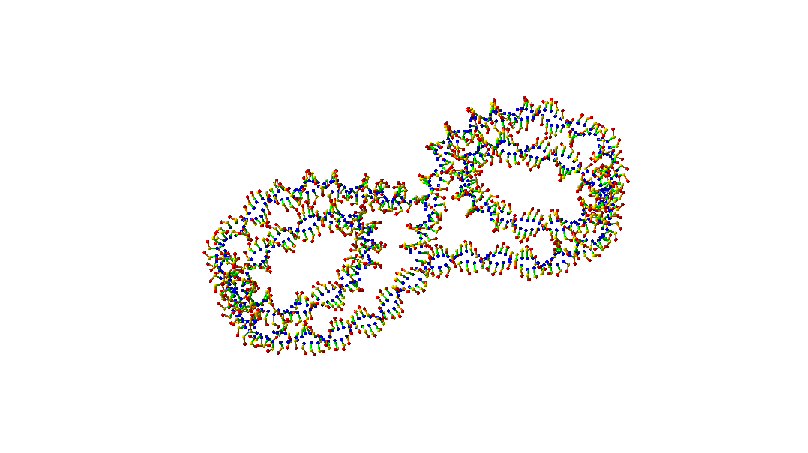
\includegraphics[width=.7\linewidth]{./Figures/re.png}
    \caption{Residuos}
    \label{fig:re}
\end{figure}

\subsubsection{Simulación}
Debido a que Geant4 no contiene secciones transversales definidas para ADN, las simulaciones son realizadas en agua y las deposiciones de energía resultantes son entonces alocadas en grupos de átomos constituyendo la molécula de ADN, para este propósito se hace uso de un bounding box(caja delimitadora) el cual es un volumen constituido de agua con dimensiones correspondientes a la respectiva molécula de ADN, la lista de física empleada es Geant4-DNA adaptada a micro y nano dosimetría, los procesos de esta extienden la física para electrones, hidrógeno, átomos de helio y algunos iones\cite{pdblib}.

\subsubsection{Algoritmo para encontrar el átomo más cercano}
Es necesario el uso de un algoritmo cuyo objetivo de este es alocar la deposición de energía en un elemento (azúcar base o fosfato) del nucleótido para luego deducir rompimientos de cadena simples y rompimientos dobles.
Para empezar se forman múltiples esferas a partir del baricentro geométrico de cada nucleótido, el radio de cada esfera es la máxima distancia entre el baricentro y las coordenadas de los átomos que constituyen el nucleótido, incluyendo el máximo radio de Van der Waals (1.8 Angstrom para el elemento del fósforo), si una deposición de energía es localizada en una esfera ligada un segundo proceso verifica los radios de Van der Waals, para encontrar el átomo del nucleótido más cercano a dicha deposición. debido a que las esferas ligadas de los nucleótidos se superponen, los dos nucleótidos más cercanos son incluidos en el algoritmo, cuando se cumple un evento, el algoritmo retorna la deposición de energía, la cadena de ADN, el id de nucleótido, y el id del grupo sea base, fosfato o azúcar, todo este proceso puede verse con más claridad en las figuras ~\ref{fig:deepbox} y ~\ref{fig:algoritmo}.


\begin{figure}[htbp]
    \centering
    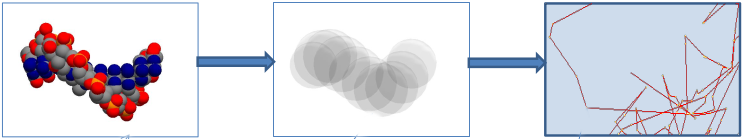
\includegraphics[width=.8\linewidth]{./Figures/aalgo.png}
    \caption[Caja delimitadora]{Caja delimitadora, lista de esferas, deposición de energía, imagen tomadas de \cite{handson} }
    \label{fig:deepbox}
\end{figure}

\begin{figure}[htbp]
    \centering
    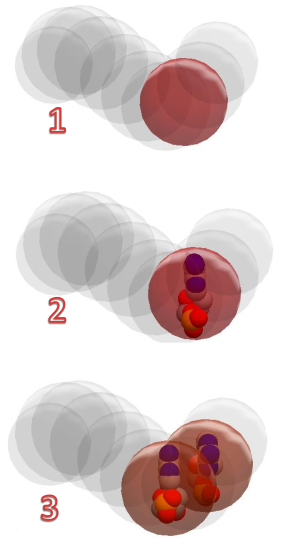
\includegraphics[width=.3\linewidth]{./Figures/algo.png}
    \caption[Esferas ligadas y nucleótidos]{Esferas ligadas y nucleótidos, imagen tomada de \cite{handson}}
    \label{fig:algoritmo}
\end{figure}

\subsubsection{Rompimientos simples y dobles}
El cálculo de rompimientos simples se hace a partir  de la asunción de que la energía sobrepase un estimado de 8.22 eV en un grupo de azúcar fosfato, es decir en un enlace fosfodiéster, para los rompimientos dobles se asume que la distancia máxima son diez pares base separando dos rompimientos simples en cadenas de ADN opuestas, cuando esto sucede se considera que ha sucedido un rompimiento doble\cite{pdblib}, esto puede ser observado en la figura ~\ref{fig:sbdb}.

\begin{figure}[htbp]
    \centering
    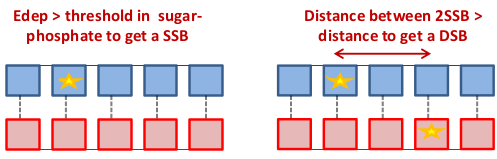
\includegraphics[width=.8\linewidth]{./Figures/romp.png}
    \caption[Esquema rompimientos simples y dobles en el ADN]{Esquema rompimientos simples y dobles en el ADN, imagen tomada de \cite{handson} }
    \label{fig:sbdb}
\end{figure}

Al principio de la simulación se crea un registro para cada cadena de ADN, los valores de dicho registro corresponden a los id de los nucleótidos y la deposición total de energía por cada evento, lo cual se tiene correlación al seguimiento de una partícula primaria y todas sus  segundarías, los registros son actualizados cada vez que el algoritmo para encontrar el átomo más cercano se completa correctamente, al final de cada evento, los registros son leídos para computar el número de rompimientos simples y dobles, cuando la simulación termina se almacena  en un histograma de ROOT la energía total de deposición en la caja de agua, y el número de rompimientos simples y dobles\cite{pdblib}, como muestra la figura ~\ref{fig:histosbdb}.

\begin{figure}[htbp]
    \centering
    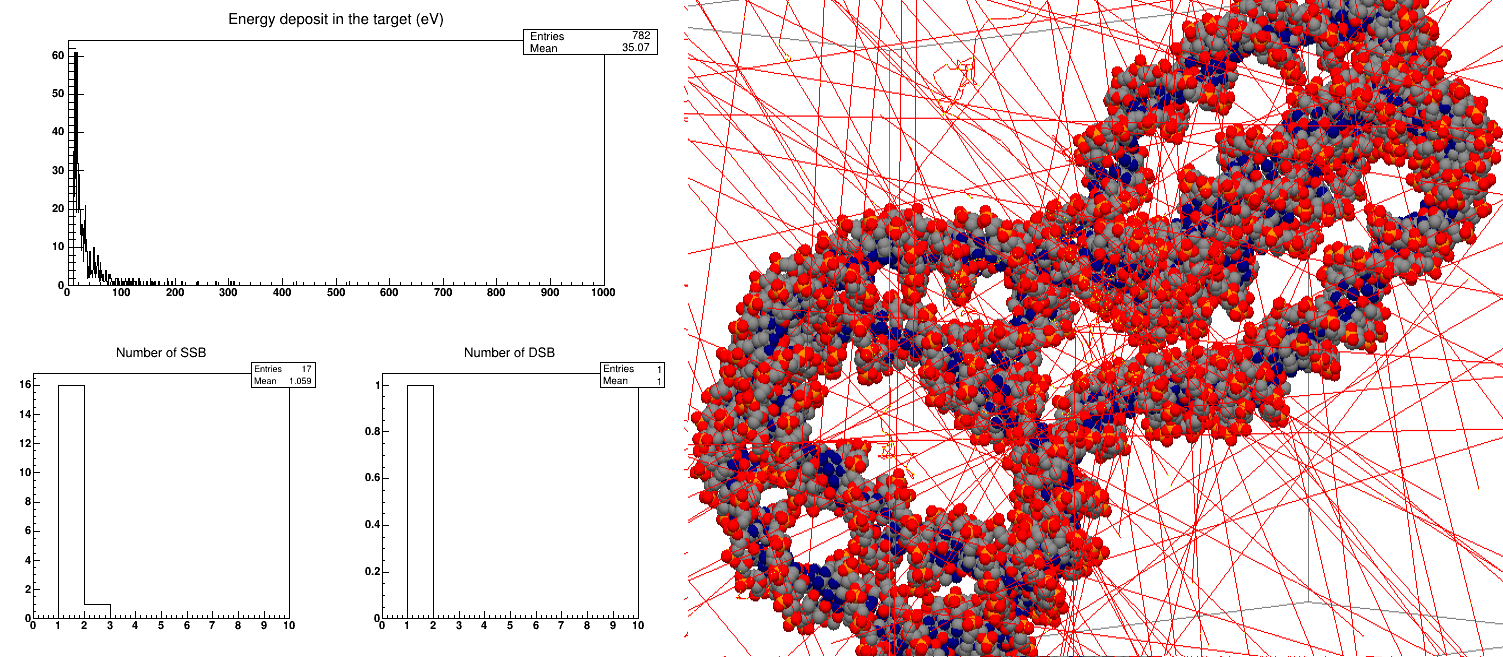
\includegraphics[width=1\linewidth]{./Figures/c1.png}
    \caption[Histograma de Root]{Histograma de Root y visualización en Geant4}
    \label{fig:histosbdb}
\end{figure}

\subsubsection{Archivos Relevantes}
Todos los ejemplos de Geant4 se componen de múltiples archivos cada uno con un propósito, esta sección aborda una explicación de los archivos fundamentales para entender pdb4dna. Un diagrama de flujo con todos los archivos de pdb4dna puede ser visto en la figura ~\ref{fig:UoC}.

\paragraph{PhysicsList}
Se encarga de llamar la física relevante para cada ejemplo, en este caso se trata de la librería "G4EmDNAPhysics" la cual contiene diversos fenómenos y procesos adaptados para nano y micro dosimetría, algunos de estos fenómenos son dispersión de Compton, dispersión de Rayleigh, efecto fotoeléctrico, etc.

\begin{figure}[htbp]
    \centering
    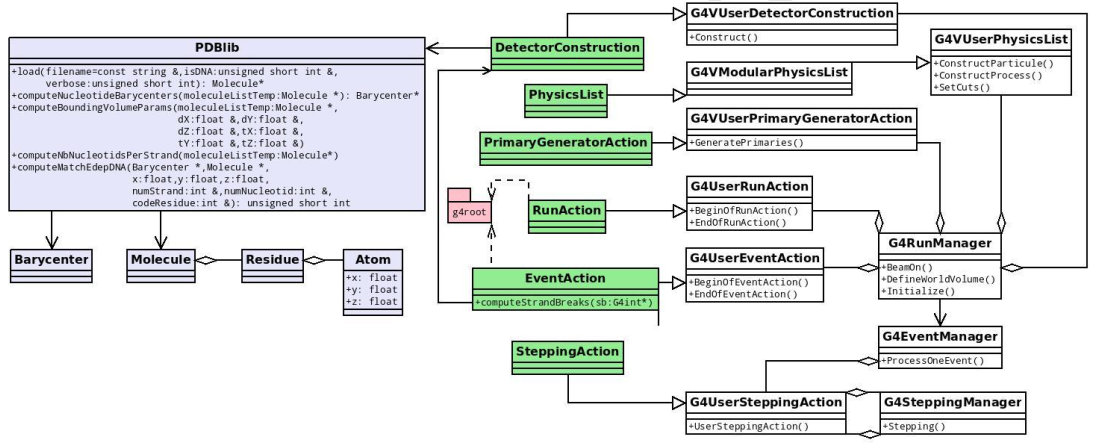
\includegraphics[width=1\linewidth]{./Figures/flujo.png}
    \caption[Diagrama de flujo de PDB4DNA]{Diagrama de flujo de PDB4DNA:Geant4 user application: Clases virtuales Geant4  (blanco), clases implementadas Geant4 (verde), librería PDB (morado) e interfaz para análisis en Root (rojo), imagen tomada de \cite{pdblib}.}
    \label{fig:UoC}
\end{figure}

\paragraph{PDBlib}

PDBlib es básicamente el corazón de PDB4DNA, es el encargado de leer el archivo de pdb, identificar si este es ADN, luego identifica las diferentes partes de la molécula de ADN como es la base, el fosfato, y el azúcar, y como el resto del código puede identificar estos para llevar a cabo el cálculo de rompimientos simples y dobles, además de ello se encarga de crear los diferentes tipos de visualización los cuales son exportados a DetectorConstruction, contiene el algoritmo para encontrar el átomo más cercano a la deposición de energía ya mencionado anteriormente.



\paragraph{DetectorConstruction}
En Geant4 este archivo se encarga de crear y posicionar los diferentes volúmenes que sean relevantes para la simulación, en el ejemplo pdb4dna es algo curioso que DetectorConstruction funciona como un archivo más de visualización para crear diferentes representaciones de la molécula de ADN, tal como se observa en las figuras: ~\ref{fig:ba}, ~\ref{fig:cpk}, ~\ref{fig:re}, sin embargo es pertinente mencionar que igual mantiene su objetivo de controlar características relevantes para la simulación como el tamaño del mundo( volumen madre donde se encuentran otros volúmenes) y el bounding box ya mencionado anteriormente.


\paragraph{SteppingAction}
Es el encargado de seguir la deposición de energía en el bounding box, primero el PDBlib se encarga de asignar un numero en base a la estructura del ADN es decir se asignan los valores numéricos: 0 para el fosfato, 1 para el azúcar y 2 para la base, esto se realiza mediante la estructura del pdb, cuando se corre un evento SteppingAction se encarga de calcular la deposición de energía en cada uno de estos, debido a que es un enlace fosfodiéster el programa solo retorna los valores de energía depositados en el fosfato o el azúcar, estos valores son enviados a subsecuentes librerías las cuales se encargan de realizar un conteo que consiste en que si la energía sobrepasa el valor de 8.22 eV cuenta como un rompimiento simple y si en 10 pares base en la cadena opuesta se presenta otro rompimiento se toma como rompimiento doble, como se muestra en la figura ~\ref{fig:sbdb}, luego todos estos datos para múltiples eventos son enviados a un archivo Root para la visualización del histograma.


% SEC5

\clearpage

\section{Explorando PDB4DNA}
\label{sec:MODIFI}
\begin{figure}[htbp]
    \centering
    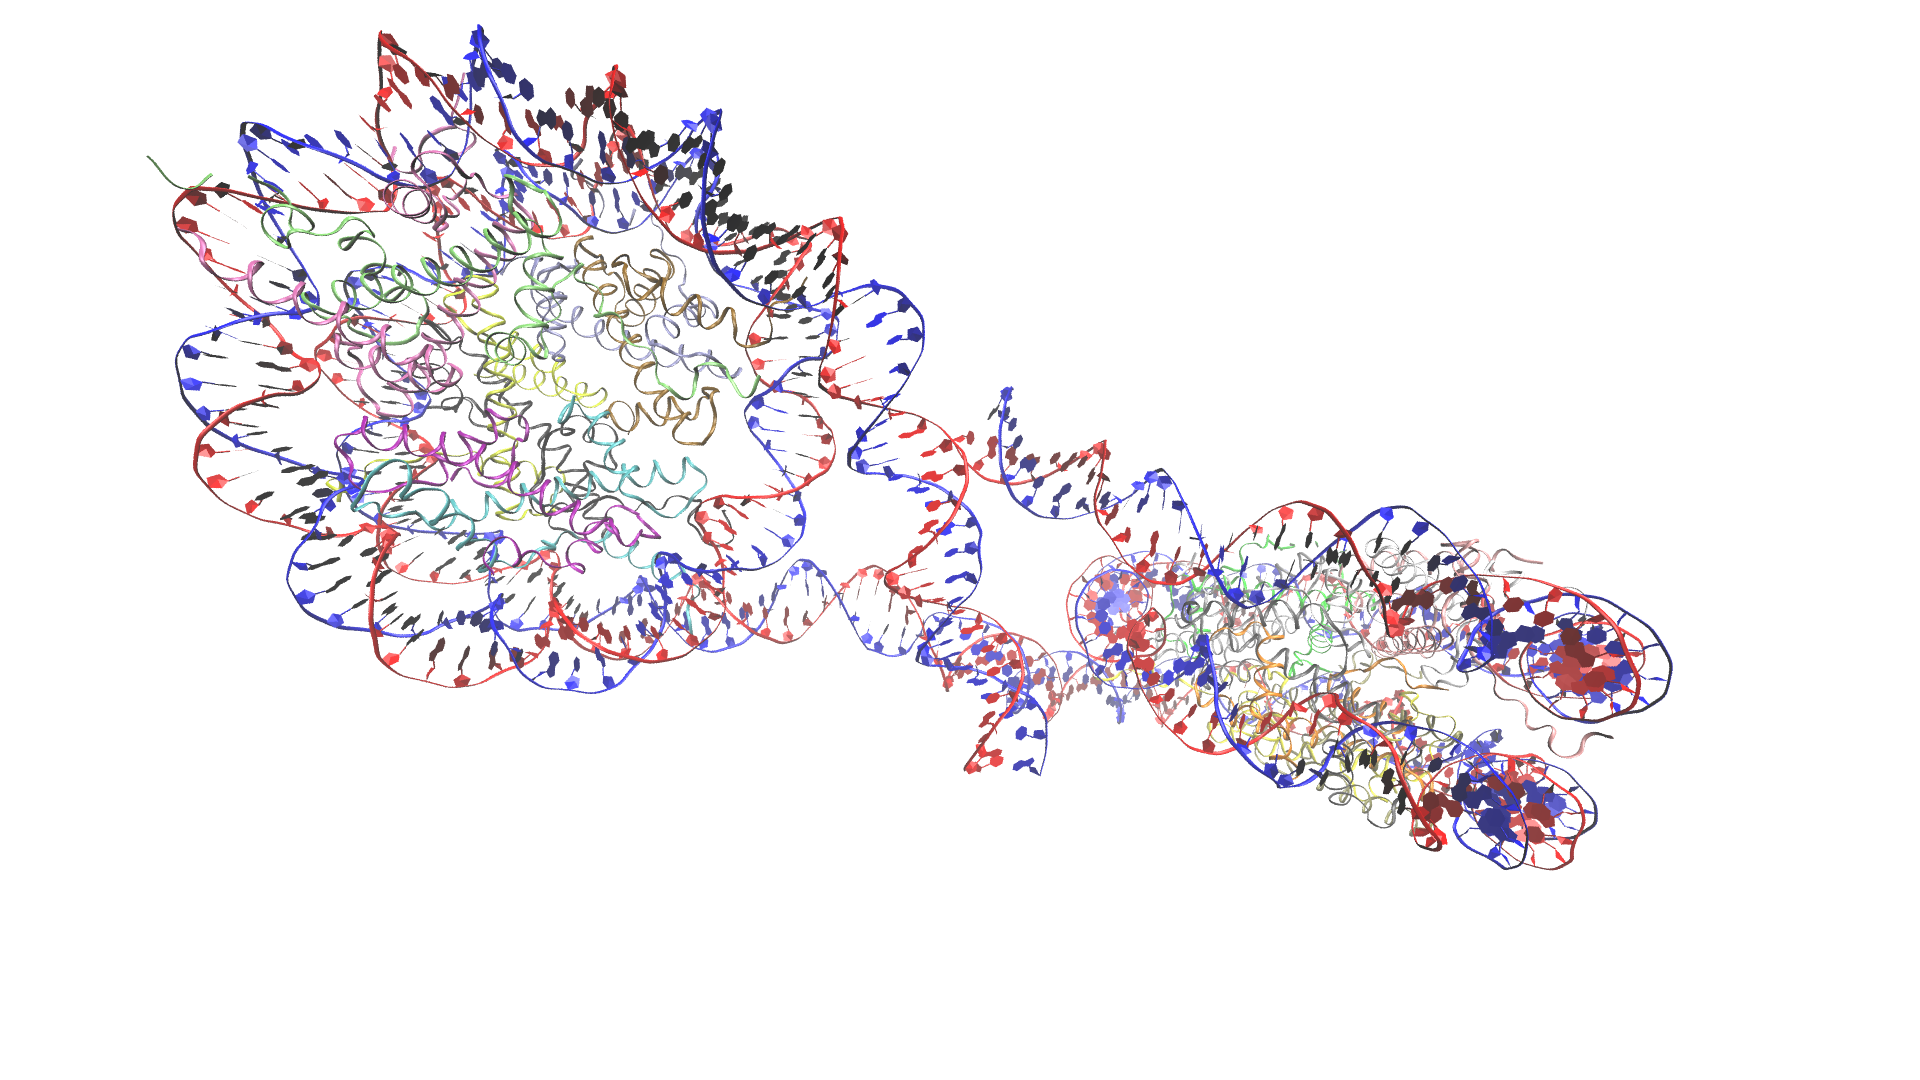
\includegraphics[width=0.8\linewidth]{./Figures/1ZBB.png}
    \caption[Molécula de ADN 1ZBB]{Molécula de ADN 1ZBB vista en VMD}
    \label{fig:1zbb}
\end{figure}

\begin{figure}[htbp]
    \centering
    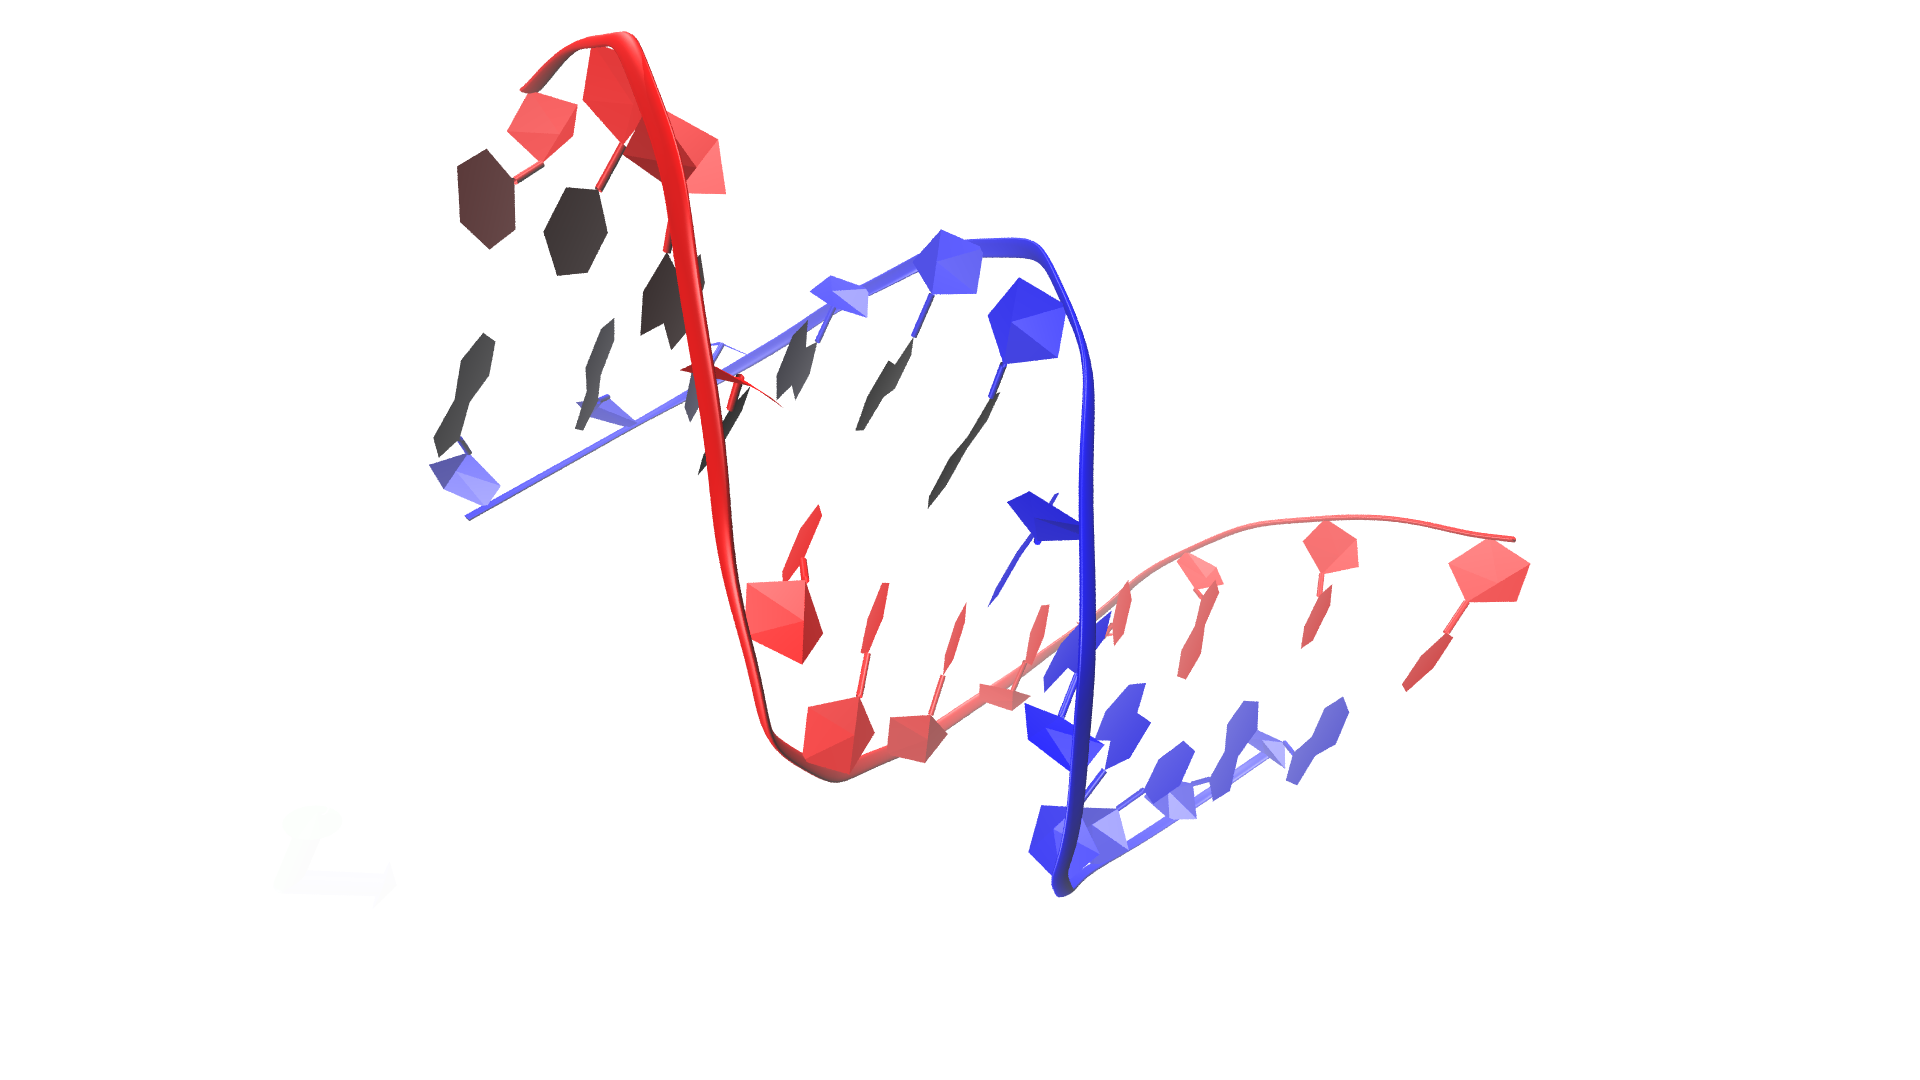
\includegraphics[width=0.8\linewidth]{./Figures/1FZX.png}
    \caption[Molécula de ADN 1FZX]{Molécula de ADN 1FZX vista en VMD}
    \label{fig:1fzx}
\end{figure}
Con tal de entender el código de pdb4dna, sus alcances, y resultados, se hace necesario el explorarlo, para esto se hizo uso de dos diferentes moléculas de ADN, 1ZBB(véase figura ~\ref{fig:1zbb} ) y 1FZX(véase figura ~\ref{fig:1fzx}), Se generaron histogramas de deposición de energía junto con los rompimientos simples y dobles, estos se realizaron con 10000 eventos con diferentes valores de energía para un electrón y un baryon con nombres en Geant4 e- y proton respectivamente, véase figuras ~\ref{fig:e}, ~\ref{fig:p}, ~\ref{fig:e2}, ~\ref{fig:p2}, de estos histogramas es interesante notar como los rompimientos simples y doble aumentan hasta cierto valor y luego empiezan a reducirse, esto puede deberse a diversos factores como el tamaño de la molécula y en cuantos enlaces se puede depositar la energía, también es necesario mencionar que en el stepping action la energía y las posiciones donde se deposita la energía se obtiene mediante la librería step y para ser precisos con la siguiente linea de código:
\lstset {language=C++}
\begin{lstlisting}
// Get position and edep of current step
    //
    G4double x = theStep->GetPreStepPoint()->GetPosition().x()/nanometer;
    G4double y = theStep->GetPreStepPoint()->GetPosition().y()/nanometer;
    G4double z = theStep->GetPreStepPoint()->GetPosition().z()/nanometer;
G4double edepStep = theStep->GetTotalEnergyDeposit()/eV;
\end{lstlisting}

Al graficar los baricentros de 1ZBB contra estas deposiciones de la energía debido a la partícula(figura ~\ref{fig:edep}) se puede ver en que partes se esta depositando la energía para cierto evento con ciertas condiciones, nótese que  bien lo que hace el código es filtrar la energía para que el programa genere un histograma de deposición de energía en donde solo se deposito energía en el fosfato o el azúcar , esto lo hace mediante varias lineas de código, primero PDBlic se encarga de leer el pdb y luego de la división de base fosfato y azúcar, mediante el código:

\lstset {language=C++}
\begin{lstlisting}
if(residueListTemp->fResSeq == 1)
            {
              if(iii == 0) BSP = 0; //"Phosphate"
              else if(iii < 8) BSP = 1; //"Sugar"
              else BSP = 2; //"Base"
            }
            else
            {
              if(iii < 4) BSP = 0; //"Phosphate"
              else if(iii < 11) BSP = 1; //"Sugar"
              else BSP = 2; //"Base"
            }
\end{lstlisting}
Mediante esto se le da un valor numérico al fosfato 0, al azúcar 1 y a la base 0, luego en el stepping action si se encuentra un golpe ya sea en el azúcar o en el fosfato se retorna ese valor de energía, esto se hace mediante:
\lstset {language=C++}
\begin{lstlisting}
int numStrand=0;
  int numNucl=0;
  int intResidue=-1; // 0 for Phospat, 1 for Sugar, 2 for Base
  unsigned short int hit = (fpDetector->GetPDBlib()).ComputeMatchEdepDNA(
      fpDetector->GetBarycenterList(),
      fpDetector->GetMoleculeList(),
      x*10., y*10., z*10.,// x10 => angstrom<->nm
      numStrand, numNucl, intResidue);

  if (hit==1)
  {
    if ((intResidue==0)||(intResidue==1)) //Edep in Phosphate or Sugar
    {
      fpEventAction->AddEdepToNucleotide(numStrand,numNucl,edepStep);
      return true;
    }
    else
    {
      return false;
    }
    \end{lstlisting}

    De modificarse lo anterior reemplazando por intResidue=2 se puede analizar deposición de energía en las bases, además de esto se podría hallar una forma de recolectar datos sobre donde se realizaron los rompimientos y con ello se podría hacer uso de gromacs para estudiar la dinámica estructural de la molécula de ADN luego de la radiación realizada por Geant4, pero debido a que no tenemos noción de como se evaluá el daño por radiación en bases y por cuestiones de tiempo, esto no se llevara acabo por el momento.



\begin{figure}
\centering
\begin{subfigure}{.5\textwidth}
  \centering
  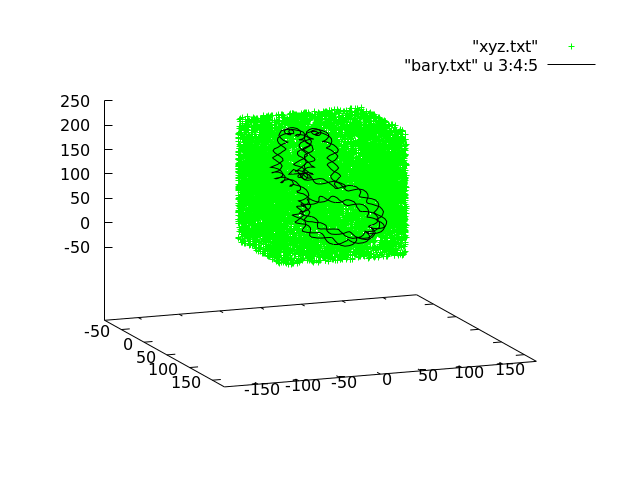
\includegraphics[width=1\linewidth]{./Figures/dep.png}
  \caption{Vista lateral}
  \label{fig:subeio1}
\end{subfigure}%
\begin{subfigure}{.5\textwidth}
  \centering
  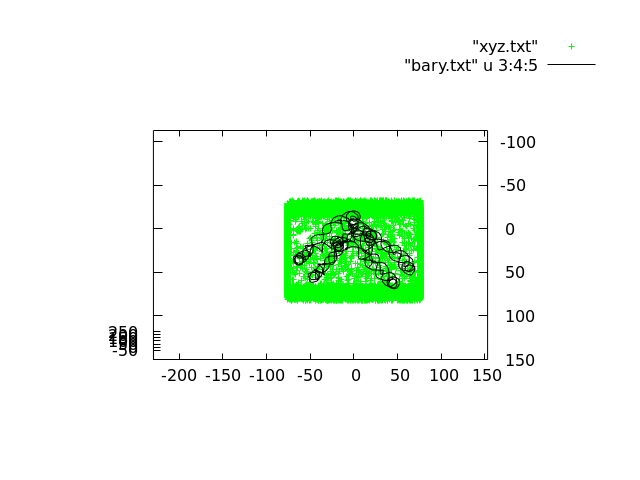
\includegraphics[width=1\linewidth]{./Figures/dep1.png}
  \caption{Vista superior}
  \label{fig:subeio2}
\end{subfigure}
\caption[Puntos de deposición de energía 1ZBB]{Puntos donde la partícula deposita energía en verde, y baricentros de 1ZBB en negro.}
\label{fig:edep}
\end{figure}




Por otro lado se tienen las limitaciones de PDB4DNA, primero que nada tiene la restricción de como leer un archivo pdb, se basa en el uso del texto "TER" encontrando en estos archivos para leer cada cadena de ADN, el problema con esto radica en que no todos los archivos de este tipo contienen este comando, además de que por el momento este numero solo permite hacer uso de moléculas de ADN de dos cadenas y filtra el resto de la molécula para que no sea leída, esto nos podemos dar cuenta al comparar la figura de 1ZBB en Geant4(figura ~\ref{h}) y la vista en vmd(figura ~\ref{fig:1zbb}) como podemos observar la vista en Geant4 no tiene en cuenta los átomos que se encuentran al interior de los anillos de 1ZBB, a pesar de ser capaz de leer moléculas diferentes a las de ADN, muchas veces no muestra estas moléculas correctamente debido en parte a lectura del termino TER y a la selección de átomos que el programa realiza para formar los nucleótidos, aunque bien de modificarse correctamente se puede hacer posible la lectura y evaluación de estás moléculas.\\
Por ultimo PDB4DNA fue modificado de tal manera que en vez de hacer uso de las esferas ligadas a partir de baricentros hiciera uso de centros de masa, para esto se uso el archivo PDBlib, primero se definió la masa de los diferentes elementos (véase anexo ~\ref{app:M}),y luego se usaron las clases bases ya definidas en PDBlib para hacer los respectivos cálculos de centros de masa(véase anexo ~\ref{app:CM})), al hacer esto y visualizar en Geant4 no se nota ningún cambio alguno para ninguna de las dos moléculas (véase figuras ~\ref{fig:sub66} y ~\ref{fig:sub666}), también al realizar los eventos con los centros de masa y generar los debidos histogramas de deposición para ambas moléculas con las mismas energías observadas en la figuras ~\ref{fig:e},~\ref{fig:p},~\ref{fig:e2},~\ref{fig:p2}, no se presenta cambio alguno y debido a esto no se incluyeron, esto se puede deber a que la influencia de la magnitud del termino de la masa no afecta en mayor medida la posición de las partículas o el programa no esta tomando correctamente los nuevos baricentros, de cualquiera manera esto requiere más estudio debido a que la inclusión de centros de masa presenta un cambio relevante al modelo propuesto por pdb4dna con el uso de baricentros,  sin embargo al hacer histogramas de Root si es posible observar cambios respecto a las posiciones que de implementarse correctamente podrían alterar resultados en las deposiciones de energía en moléculas mucho más grandes y en consecuencia en los rompimientos dobles, los histogramas fueron realizados para cada cadena de ADN y su respectivas coordenadas x,y,z, para 1ZBB véase figuras: ~\ref{fig:canx},~\ref{fig:cany},~\ref{fig:canz}, y para 1FZX: ~\ref{fig:cax},~\ref{fig:cay},~\ref{fig:caz}.


\begin{figure}
\centering
\begin{subfigure}{.5\textwidth}
  \centering
  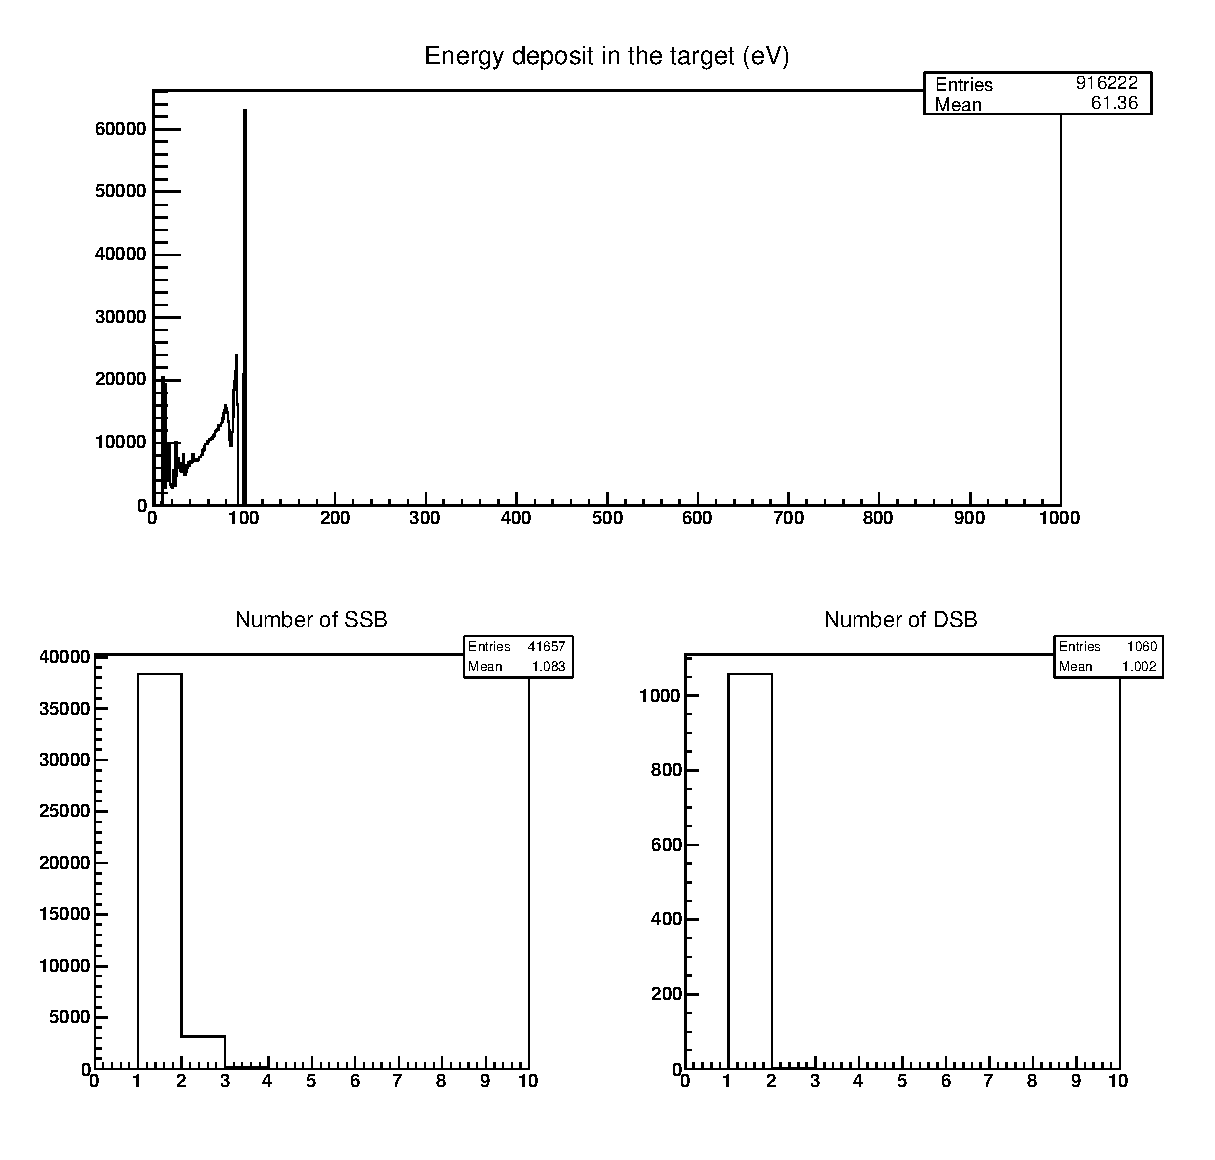
\includegraphics[width=.78\linewidth]{./Figures/1zbbe100ev.eps}
  \caption{100 eV}
  \label{fig:subei1}
\end{subfigure}%
\begin{subfigure}{.5\textwidth}
  \centering
  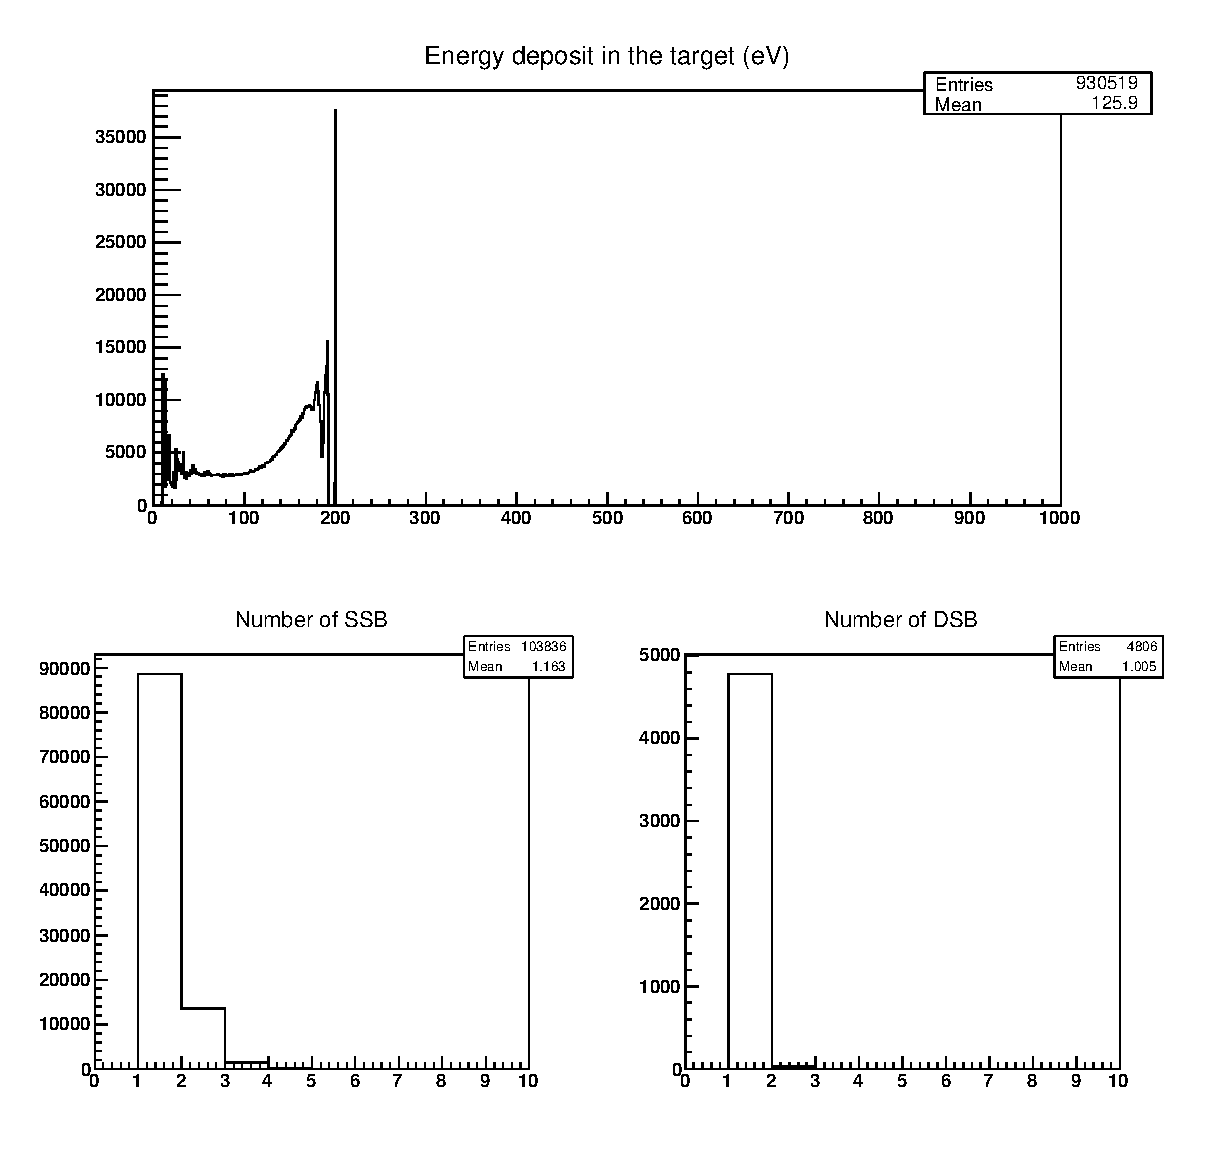
\includegraphics[width=.78\linewidth]{./Figures/1zbbe200ev.eps}
  \caption{200 eV}
  \label{fig:subei2}
\end{subfigure}
\begin{subfigure}{.5\textwidth}
  \centering
  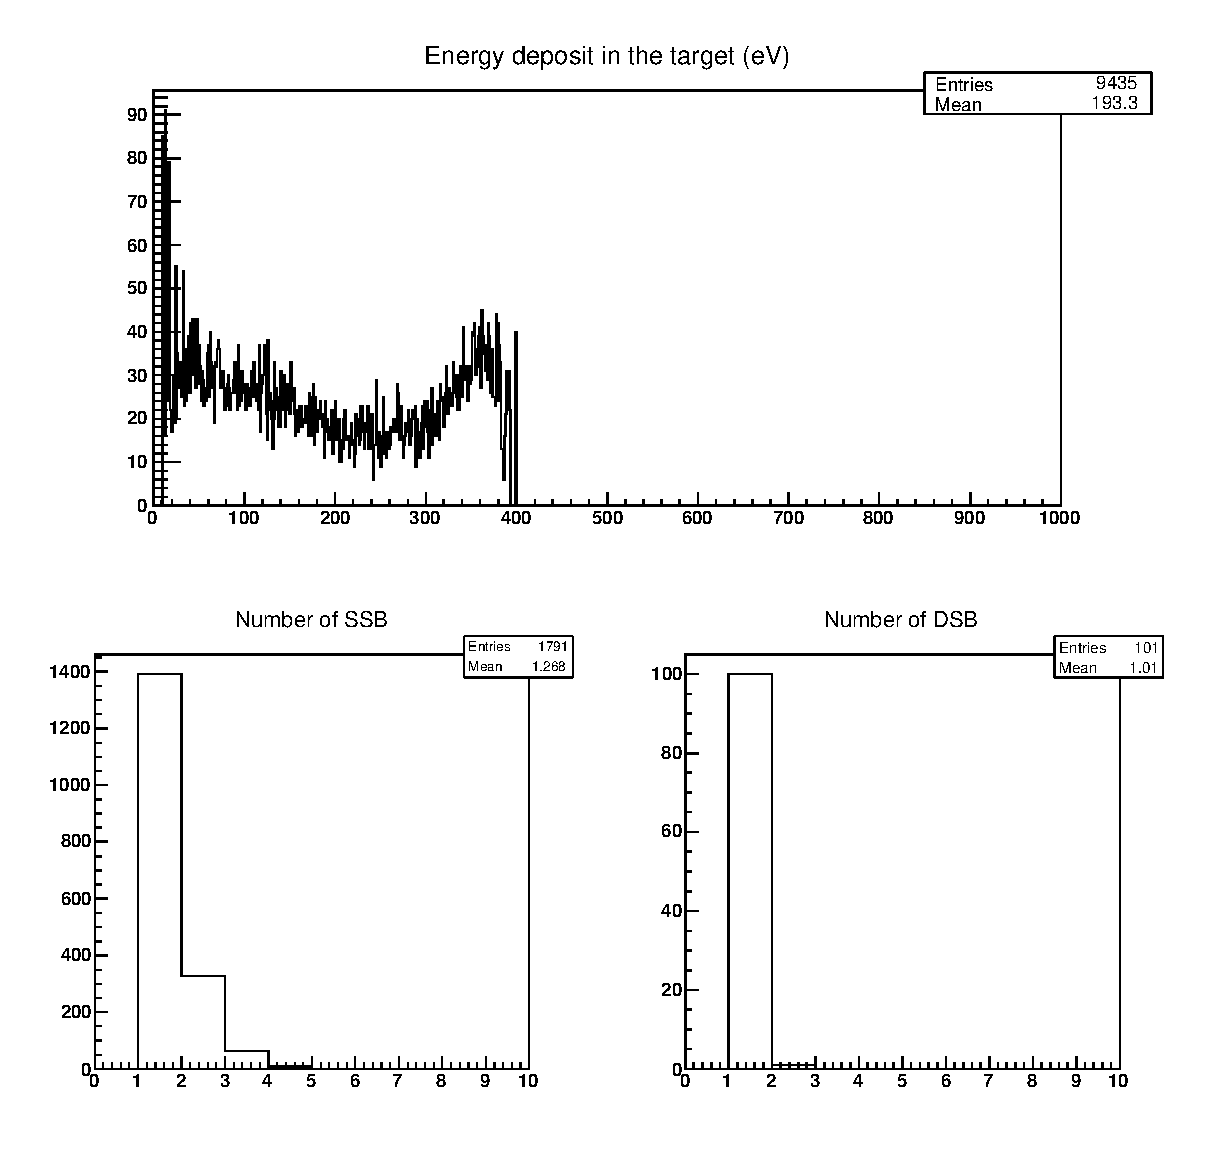
\includegraphics[width=.78\linewidth]{./Figures/1zbbe400ev.eps}
  \caption{400 eV}
  \label{fig:subei3}
\end{subfigure}%
\begin{subfigure}{.5\textwidth}
  \centering
  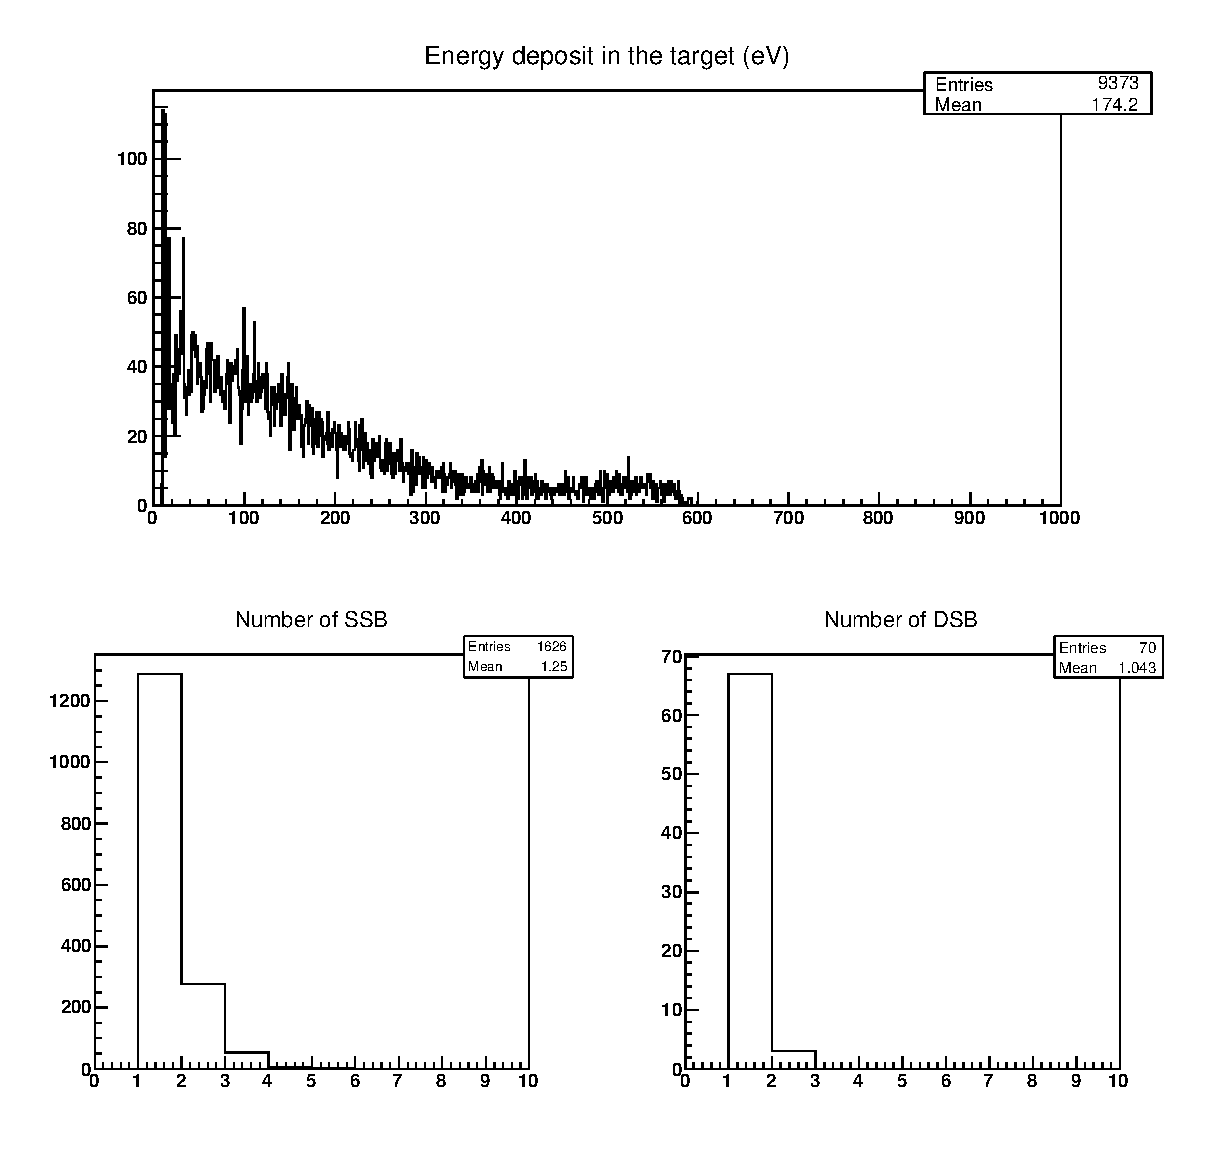
\includegraphics[width=.78\linewidth]{./Figures/1zbbe600ev.eps}
  \caption{600 eV}
  \label{fig:subei4}
\end{subfigure}
\begin{subfigure}{.5\textwidth}
  \centering
  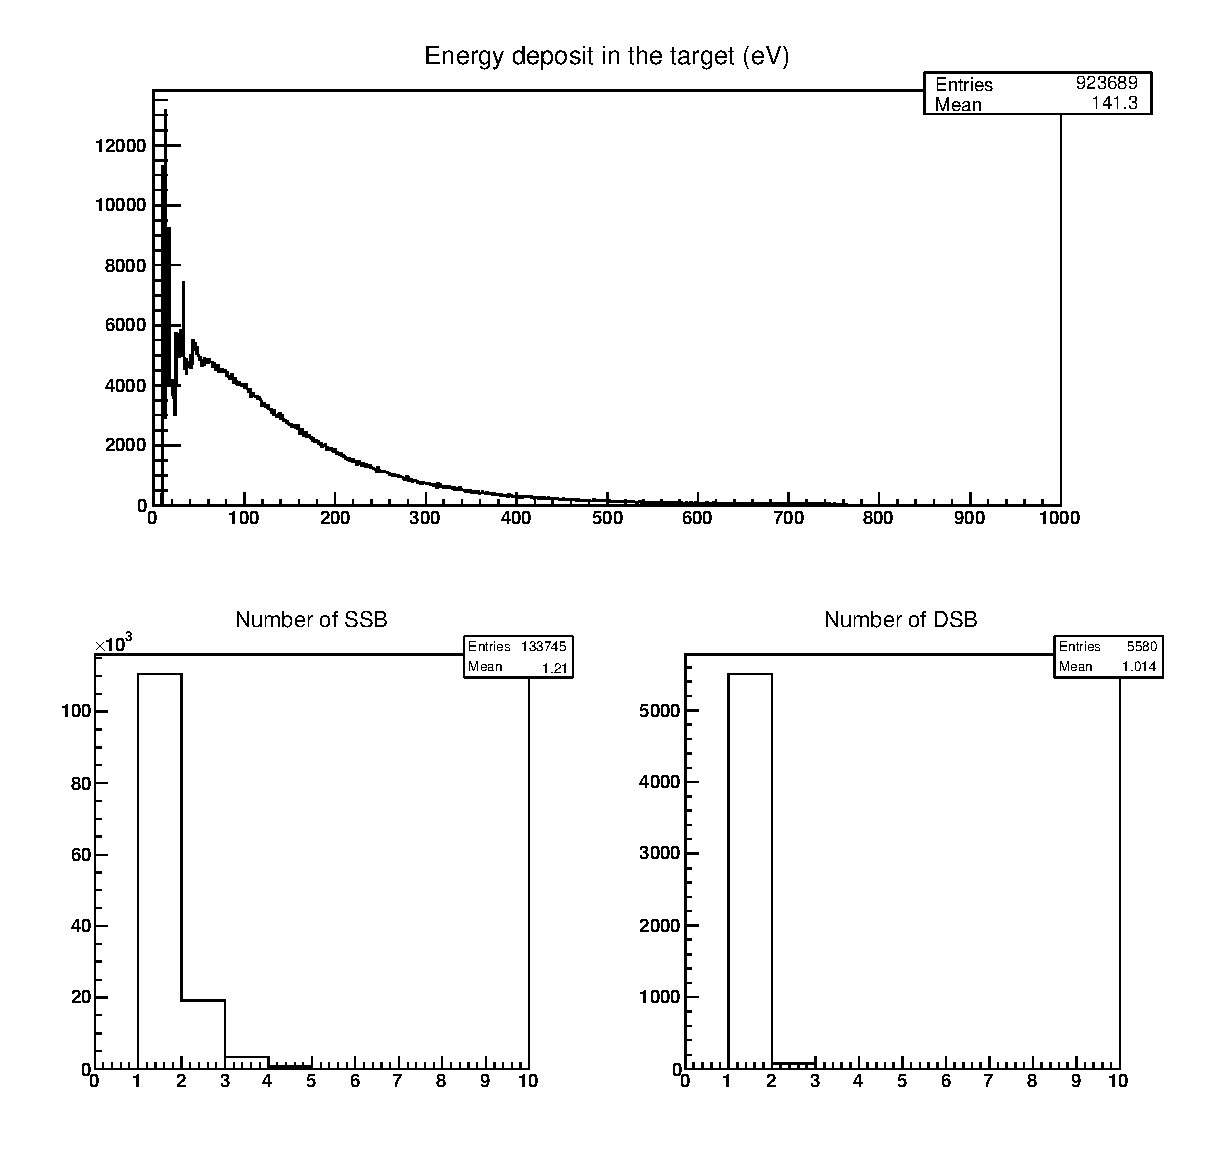
\includegraphics[width=.78\linewidth]{./Figures/1zbbe800ev.eps}
  \caption{800 eV}
  \label{fig:subei5}
\end{subfigure}%
\begin{subfigure}{.5\textwidth}
  \centering
  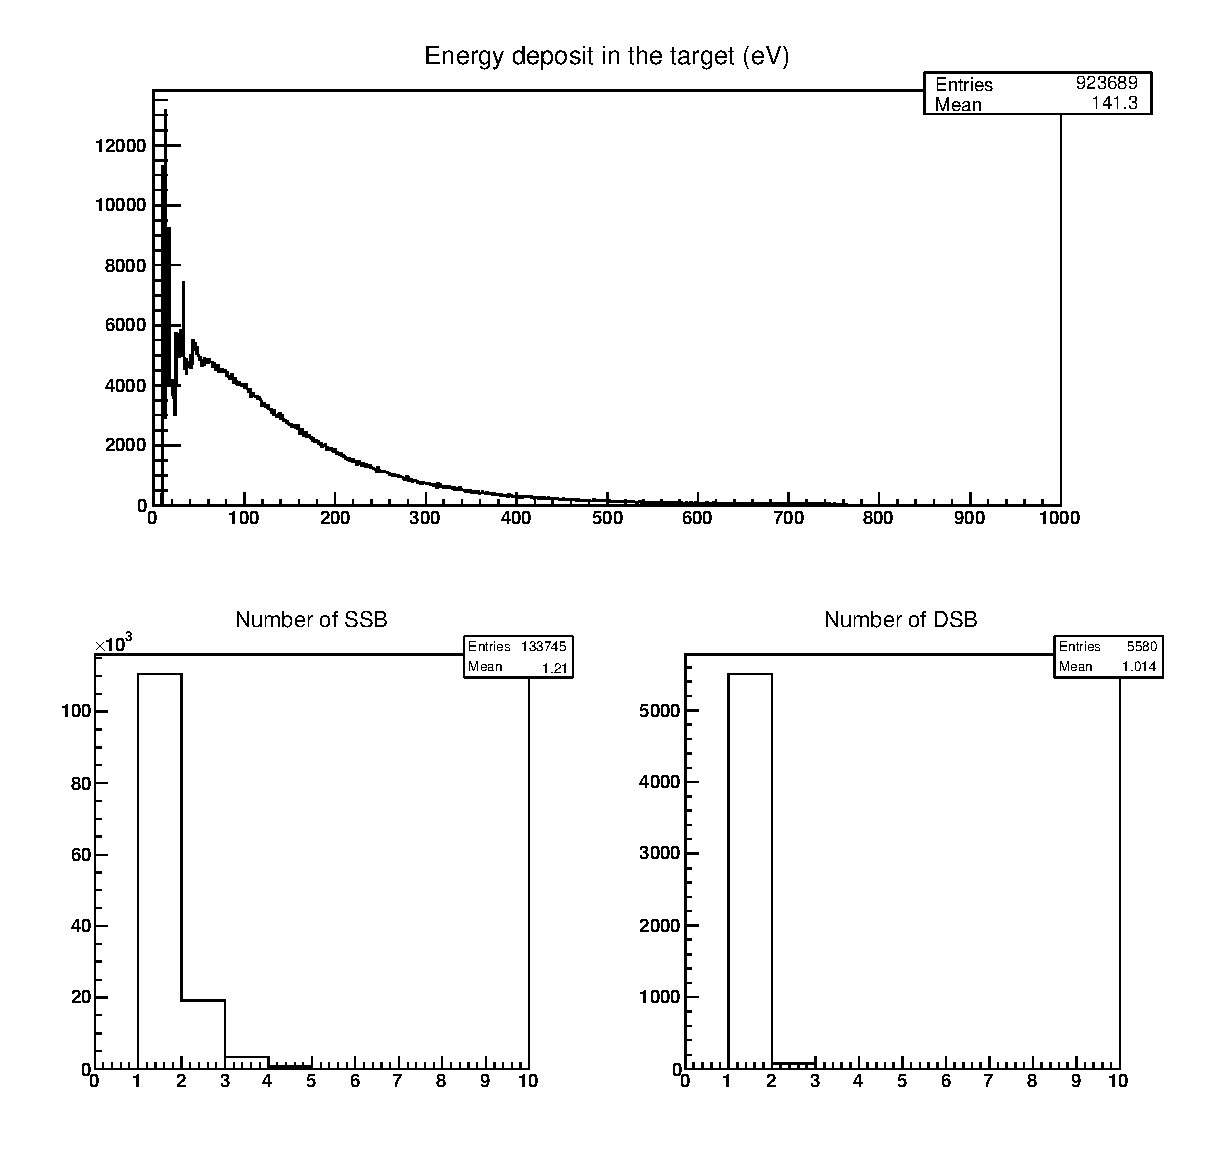
\includegraphics[width=.78\linewidth]{./Figures/1zbbe800ev.eps}
  \caption{1 keV}
  \label{fig:subei6}
\end{subfigure}
\begin{subfigure}{.5\textwidth}
  \centering
  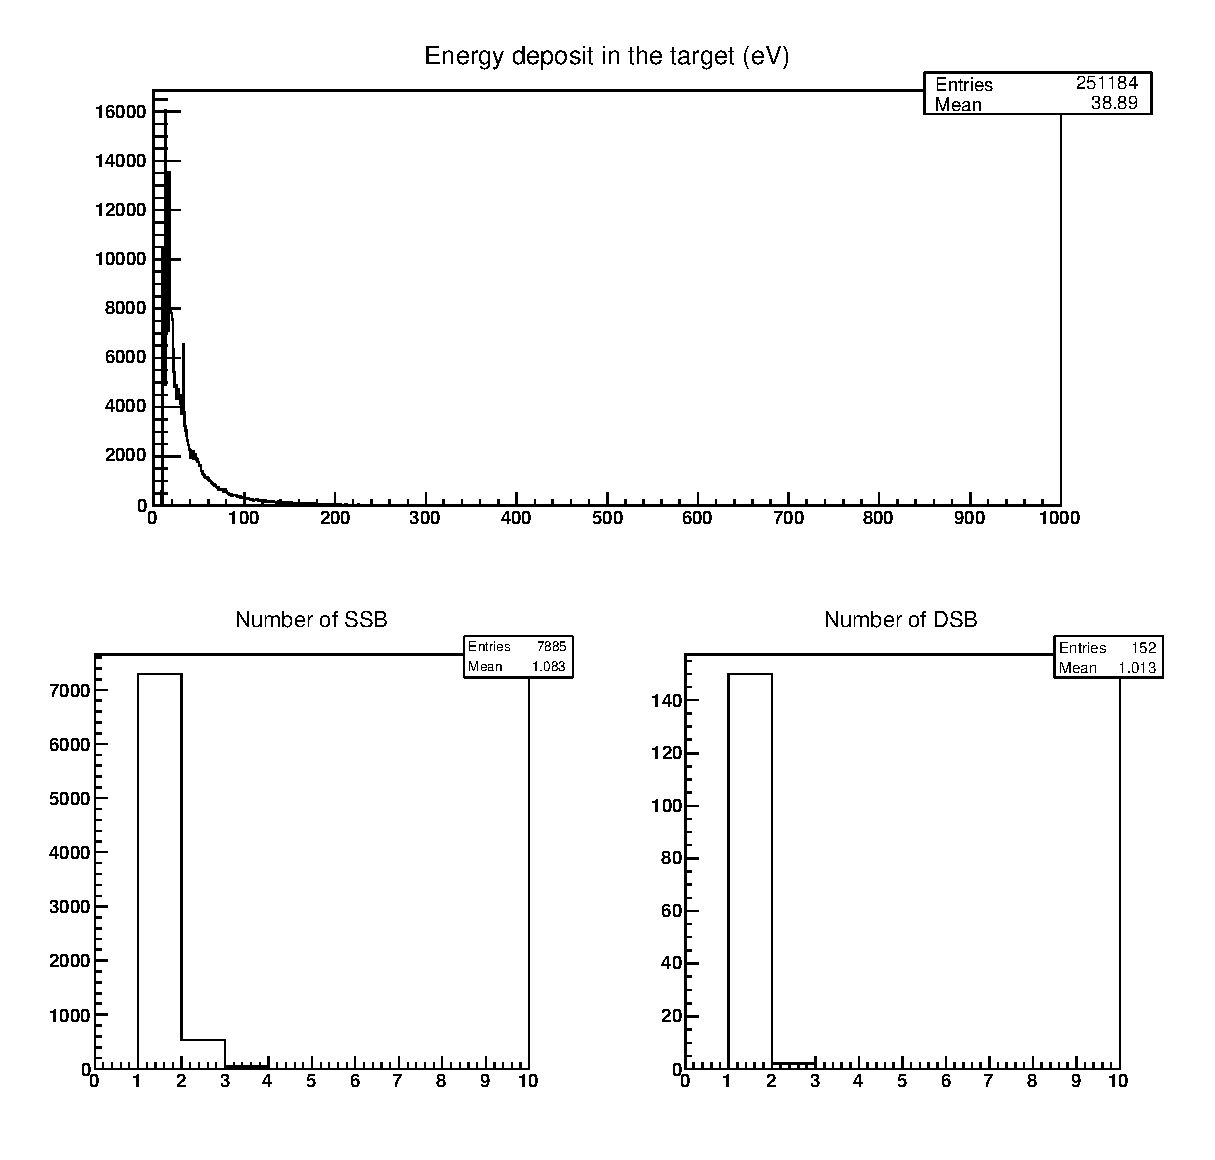
\includegraphics[width=.78\linewidth]{./Figures/1zbbe20kev.eps}
  \caption{20 keV}
  \label{fig:subei7}
\end{subfigure}%
\begin{subfigure}{.5\textwidth}
  \centering
  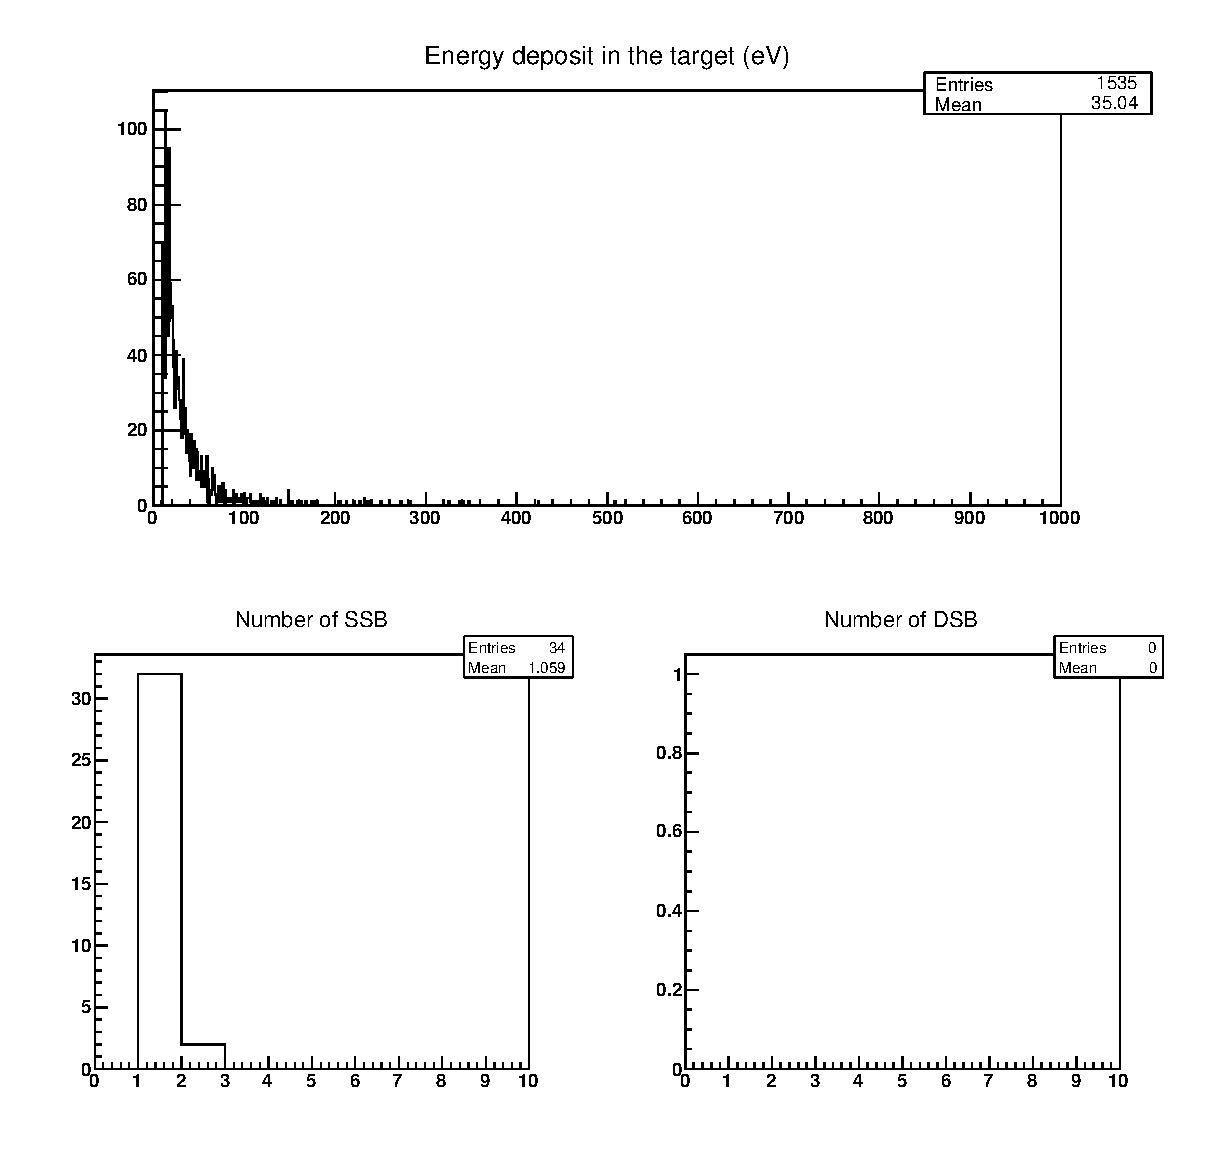
\includegraphics[width=.78\linewidth]{./Figures/1zbbe40kev.eps}
  \caption{40 keV}
  \label{fig:subei8}
\end{subfigure}
\caption{Rompimientos simples y dobles para 1ZBB ($e-$)}
\label{fig:e}
\end{figure}




\begin{figure}
\centering
\begin{subfigure}{.5\textwidth}
  \centering
  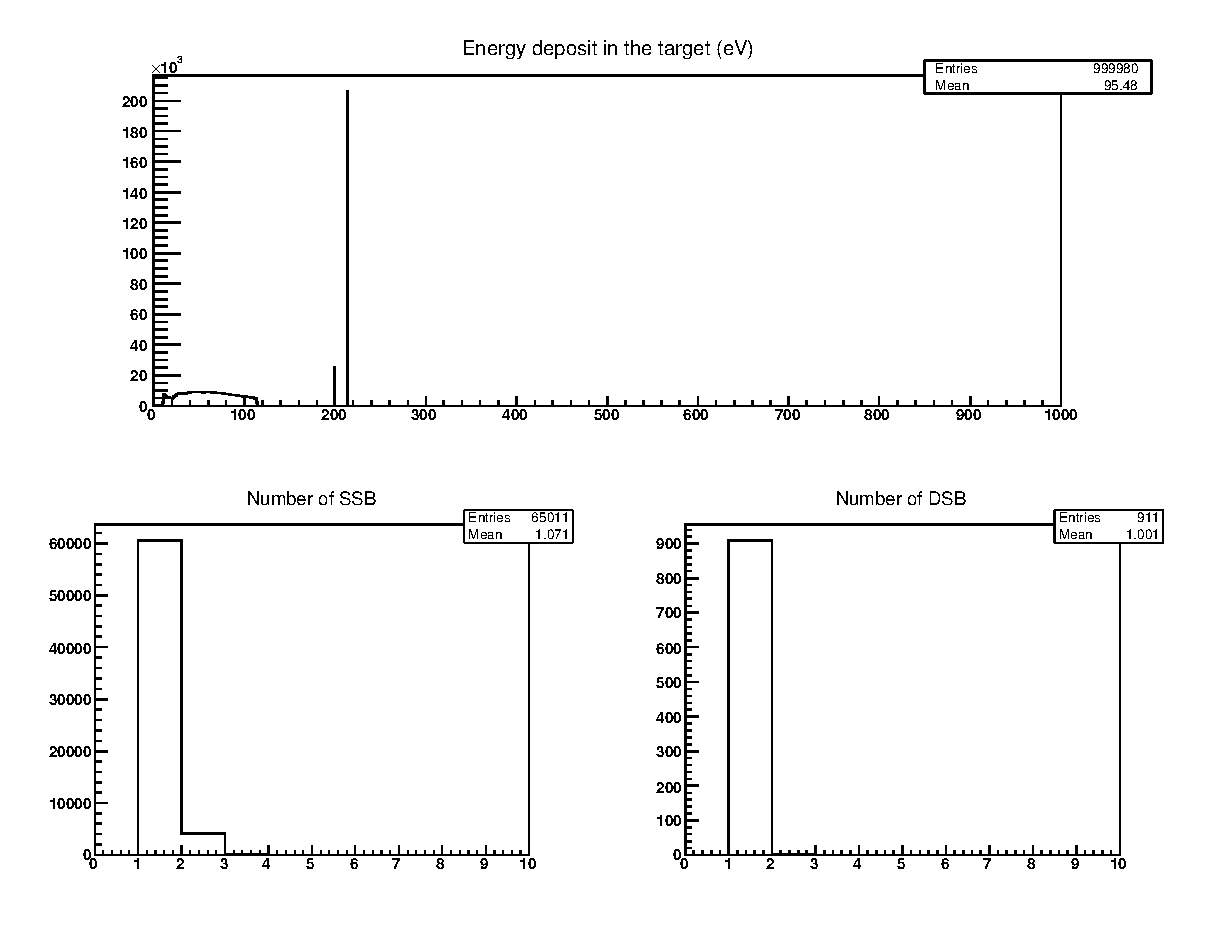
\includegraphics[width=.78\linewidth]{./Figures/1zbbp200ev.eps}
  \caption{200 eV}
  \label{fig:sub1}
\end{subfigure}%
\begin{subfigure}{.5\textwidth}
  \centering
  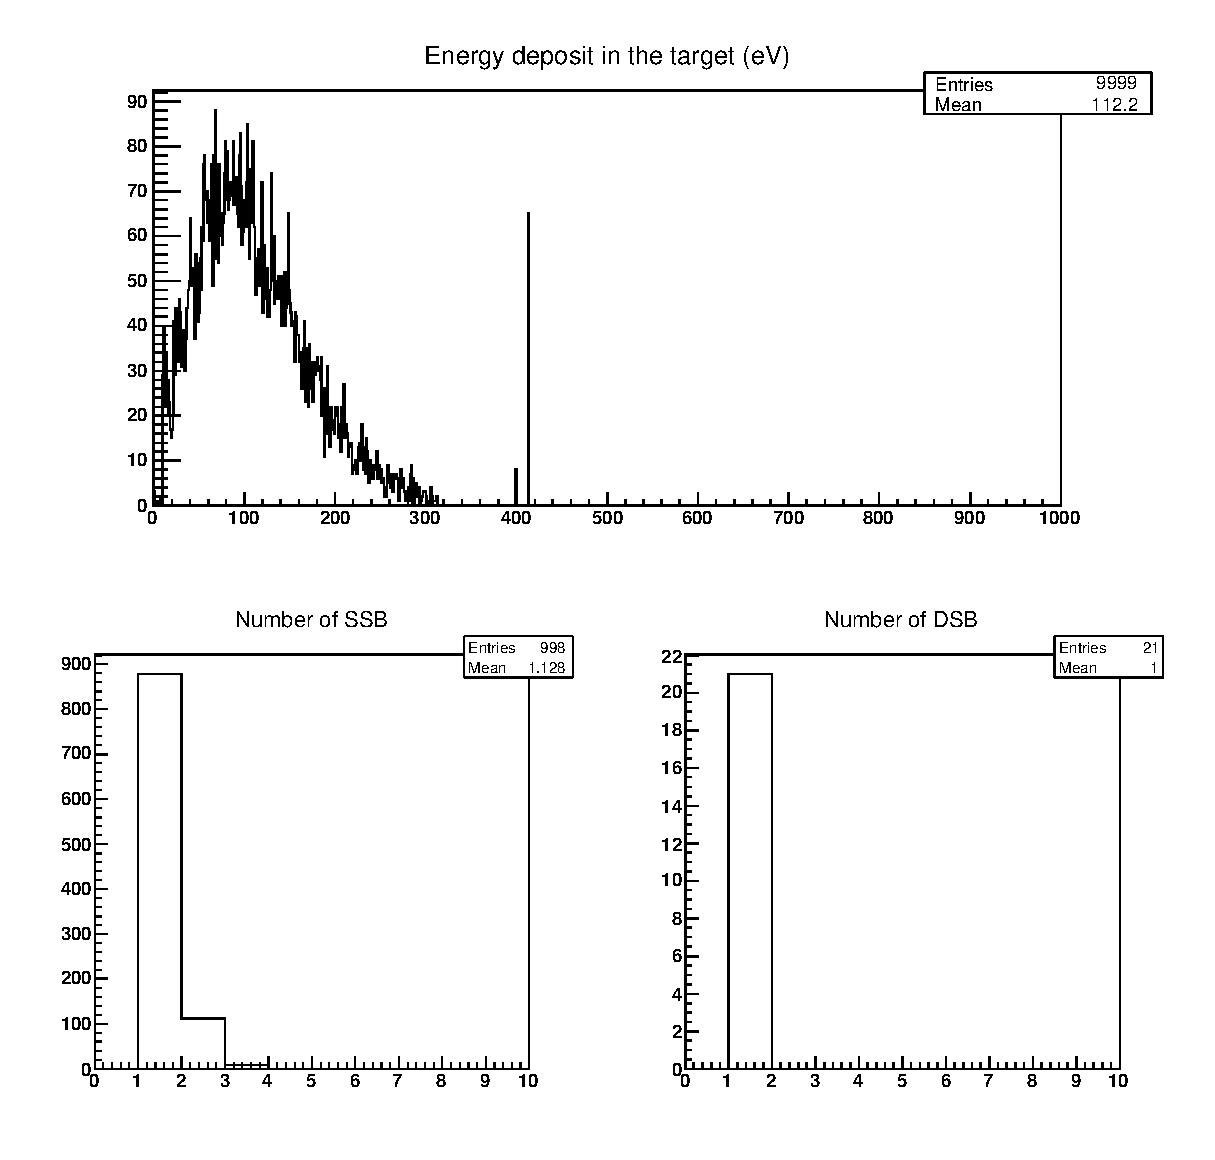
\includegraphics[width=.78\linewidth]{./Figures/1zbbp400ev.eps}
  \caption{400 eV}
  \label{fig:sub2}
\end{subfigure}
\begin{subfigure}{.5\textwidth}
  \centering
  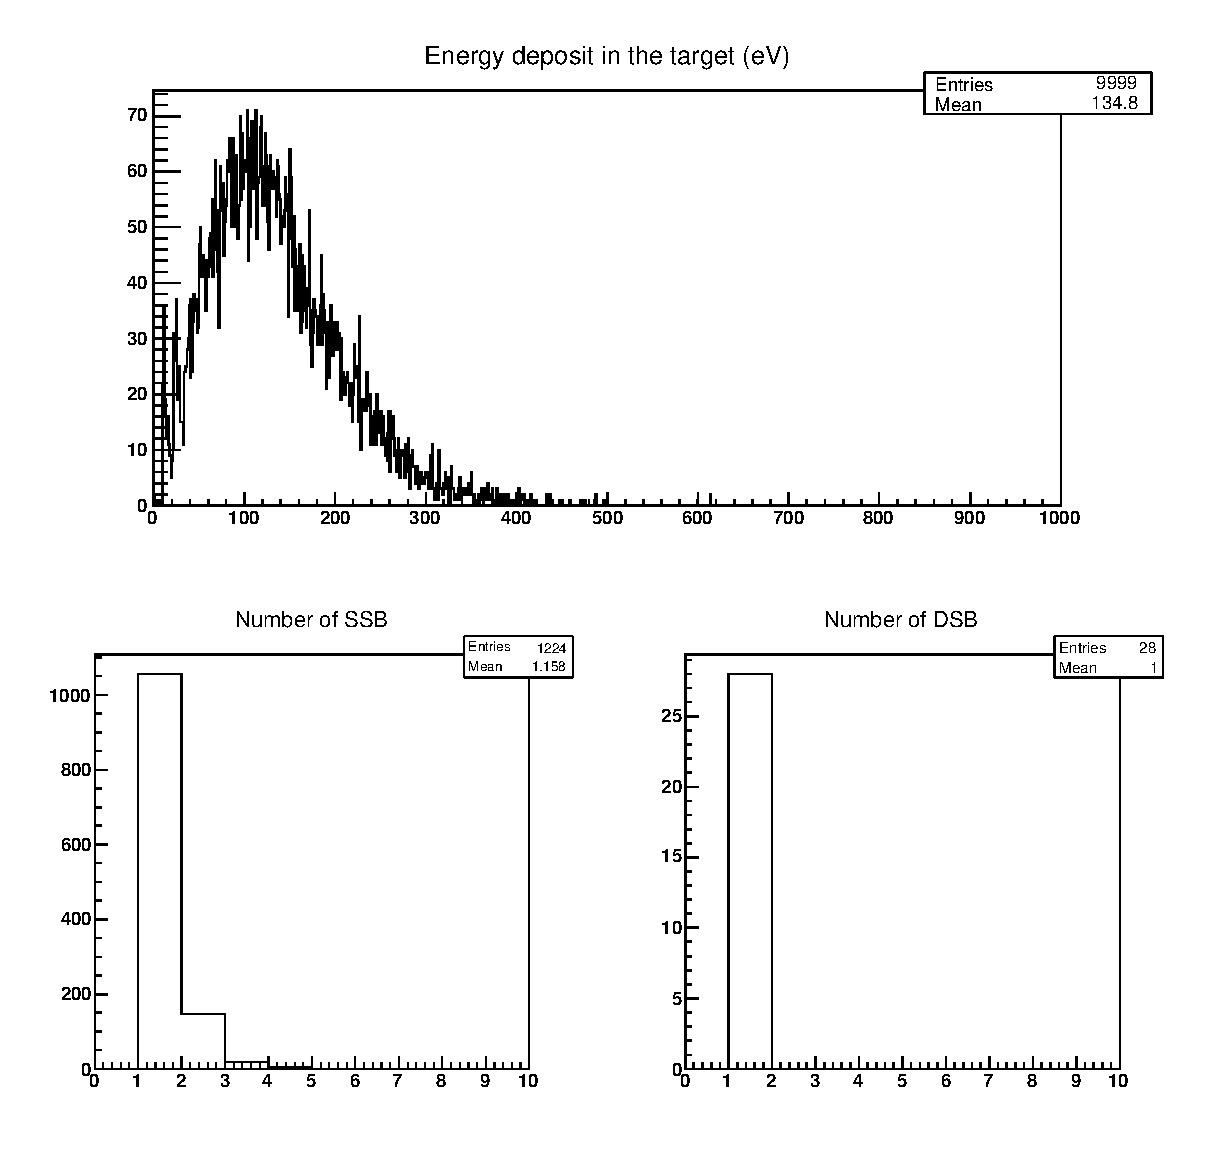
\includegraphics[width=.78\linewidth]{./Figures/1zbbp600ev.eps}
  \caption{600 eV}
  \label{fig:sub3}
\end{subfigure}%
\begin{subfigure}{.5\textwidth}
  \centering
  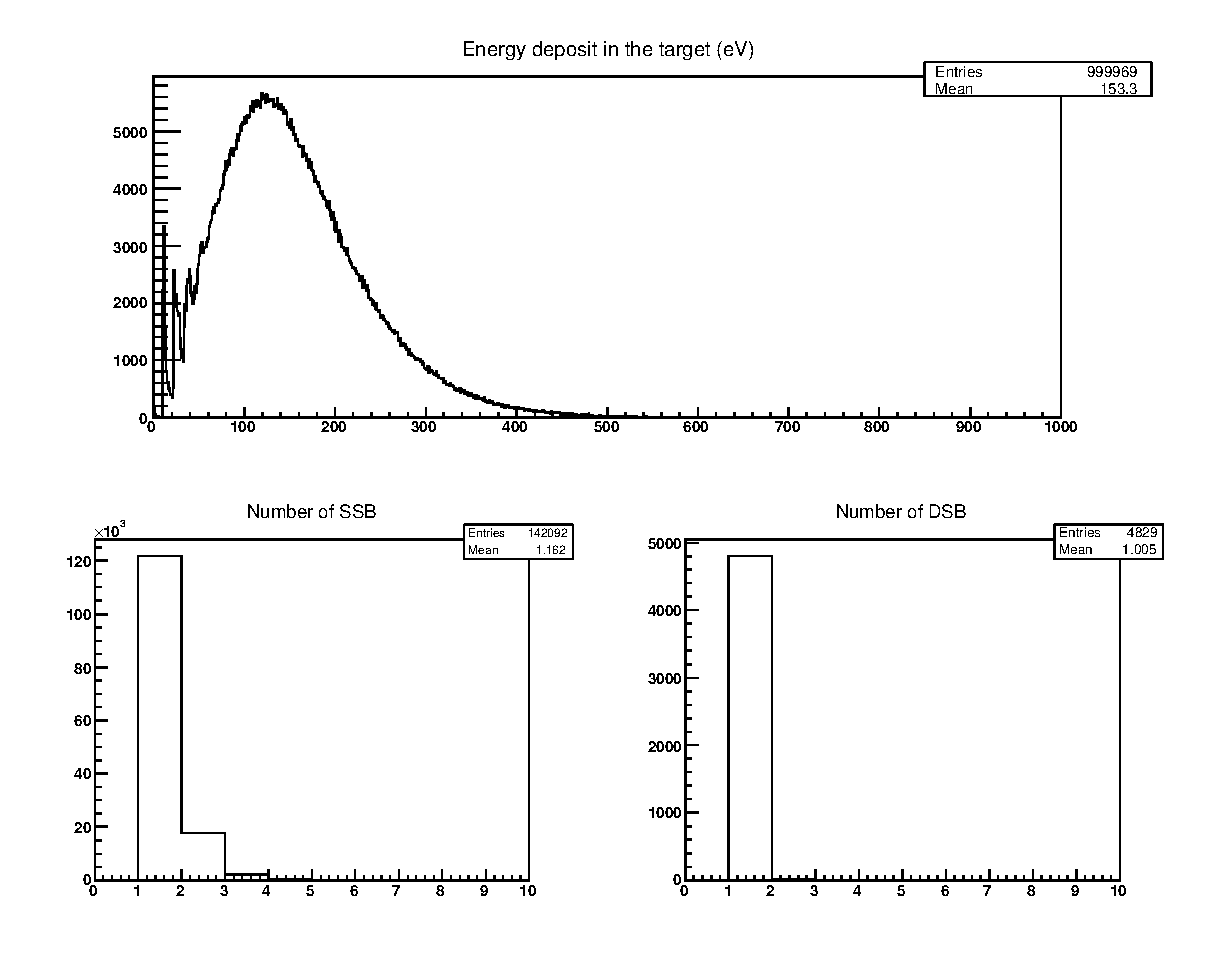
\includegraphics[width=.78\linewidth]{./Figures/1zbbp800ev.eps}
  \caption{800 eV}
  \label{fig:sub4}
\end{subfigure}
\begin{subfigure}{.5\textwidth}
  \centering
  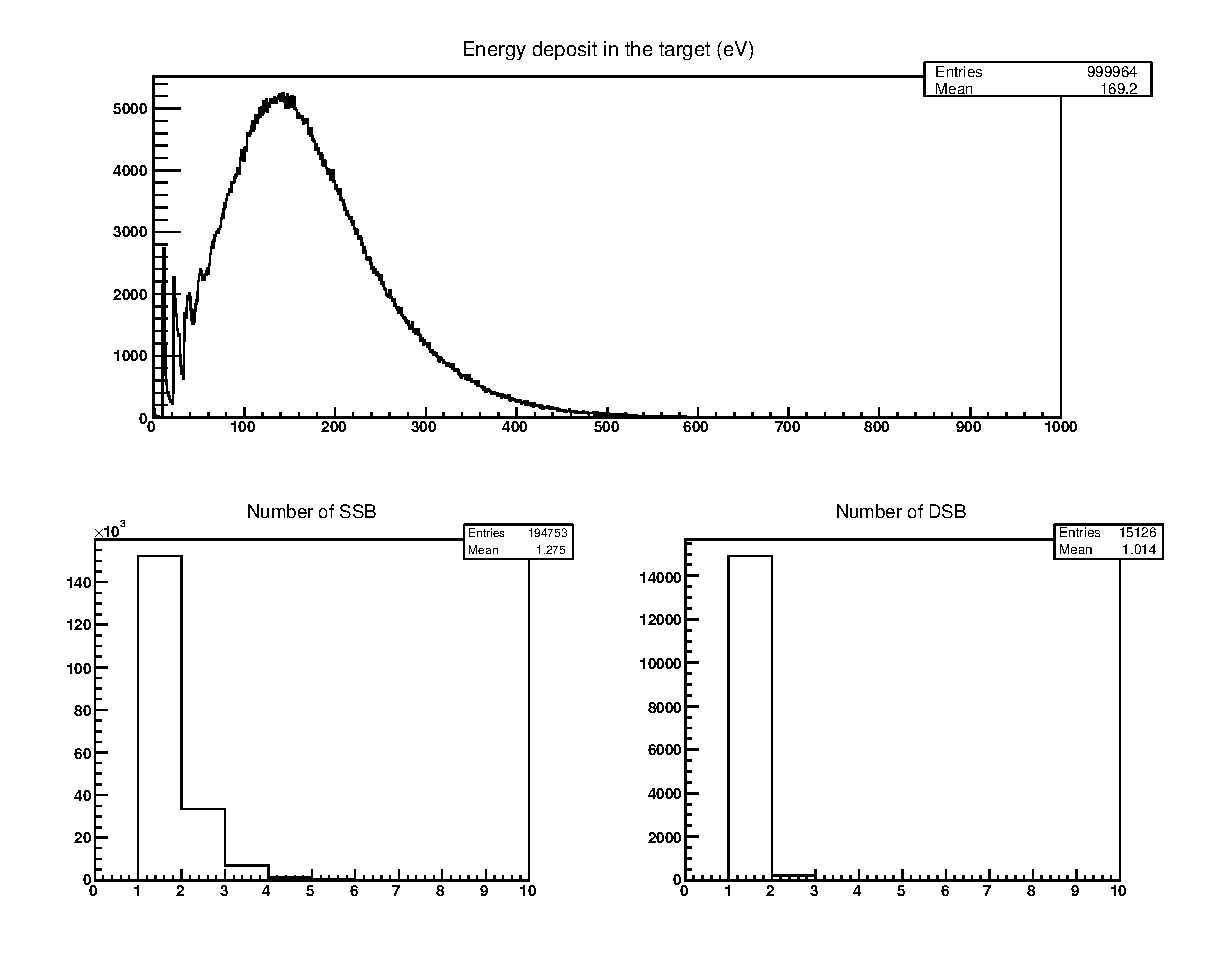
\includegraphics[width=.78\linewidth]{./Figures/1zbbp1kev.eps}
  \caption{1 keV}
  \label{fig:sub5}
\end{subfigure}%
\begin{subfigure}{.5\textwidth}
  \centering
  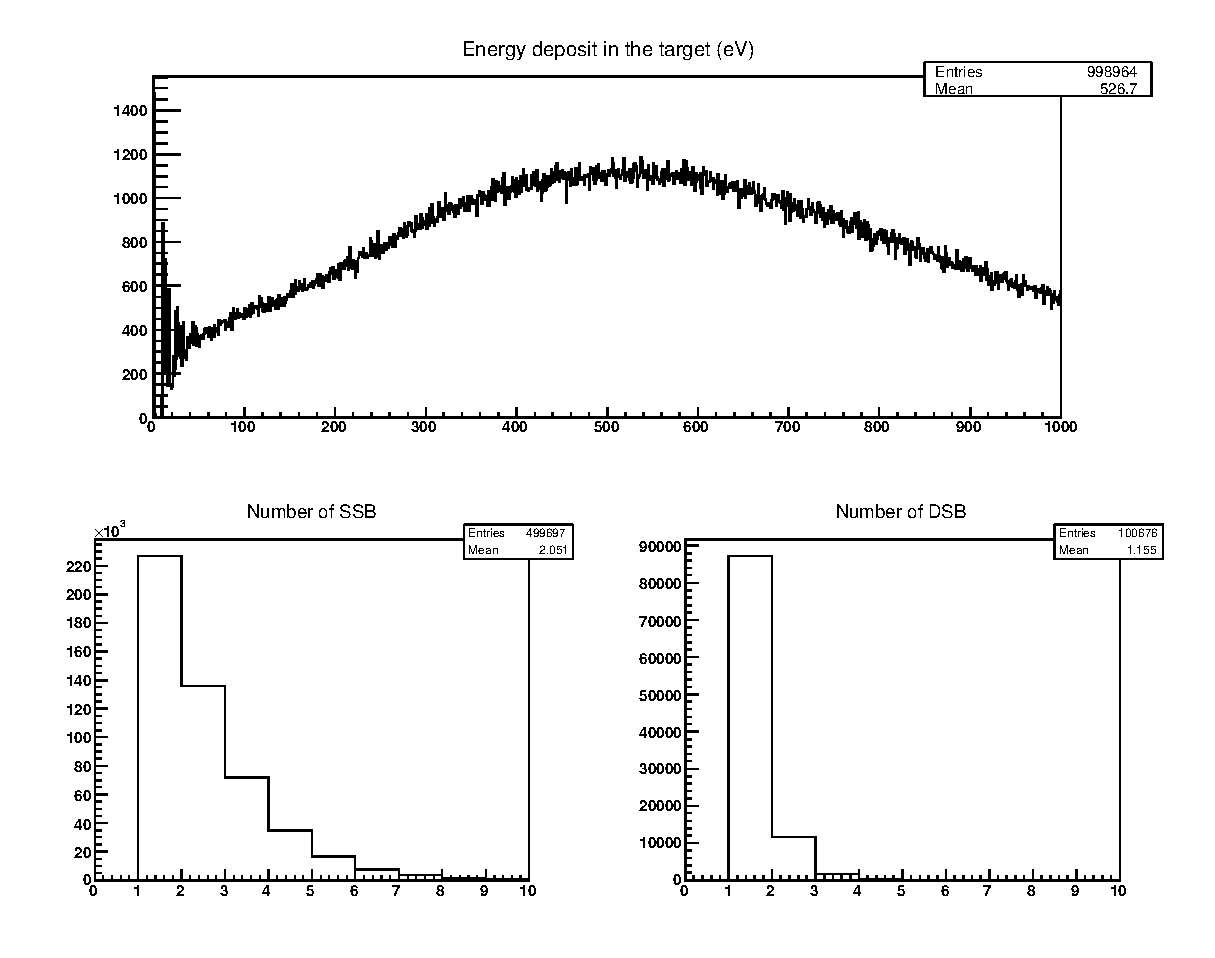
\includegraphics[width=.78\linewidth]{./Figures/1zbbp200kev.eps}
  \caption{200 keV}
  \label{fig:sub6}
\end{subfigure}
\begin{subfigure}{.5\textwidth}
  \centering
  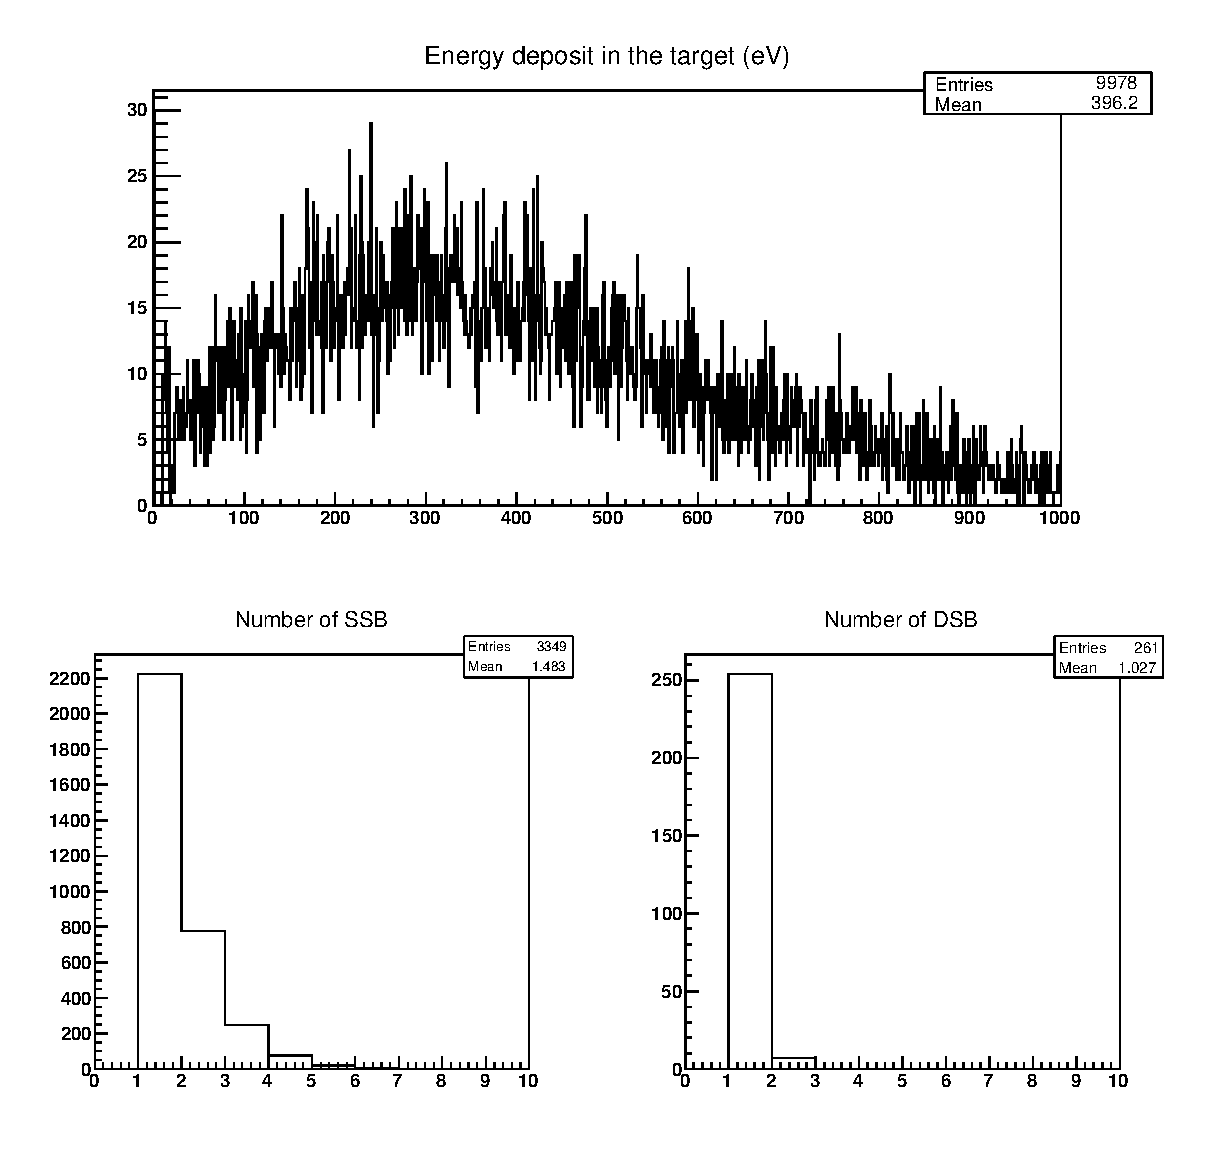
\includegraphics[width=.78\linewidth]{./Figures/1zbbp400kev.eps}
  \caption{400 keV}
  \label{fig:sub7}
\end{subfigure}%
\begin{subfigure}{.5\textwidth}
  \centering
  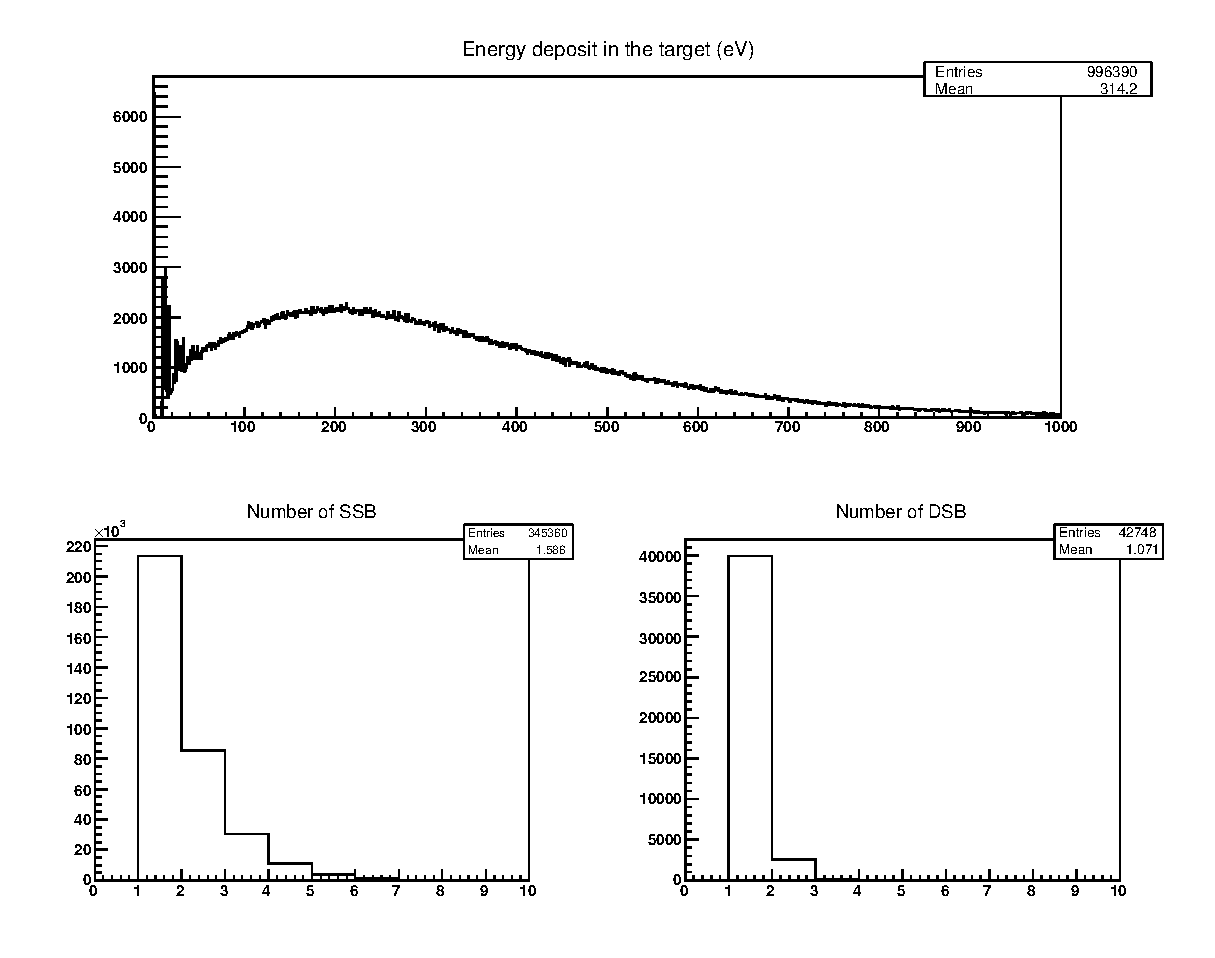
\includegraphics[width=.78\linewidth]{./Figures/1zbbp600kev.eps}
  \caption{600 keV}
  \label{fig:sub8}
\end{subfigure}
\caption{Rompimientos simples y dobles para 1ZBB ($proton$)}
\label{fig:p}
\end{figure}



\begin{figure}
\centering
\begin{subfigure}{.5\textwidth}
  \centering
  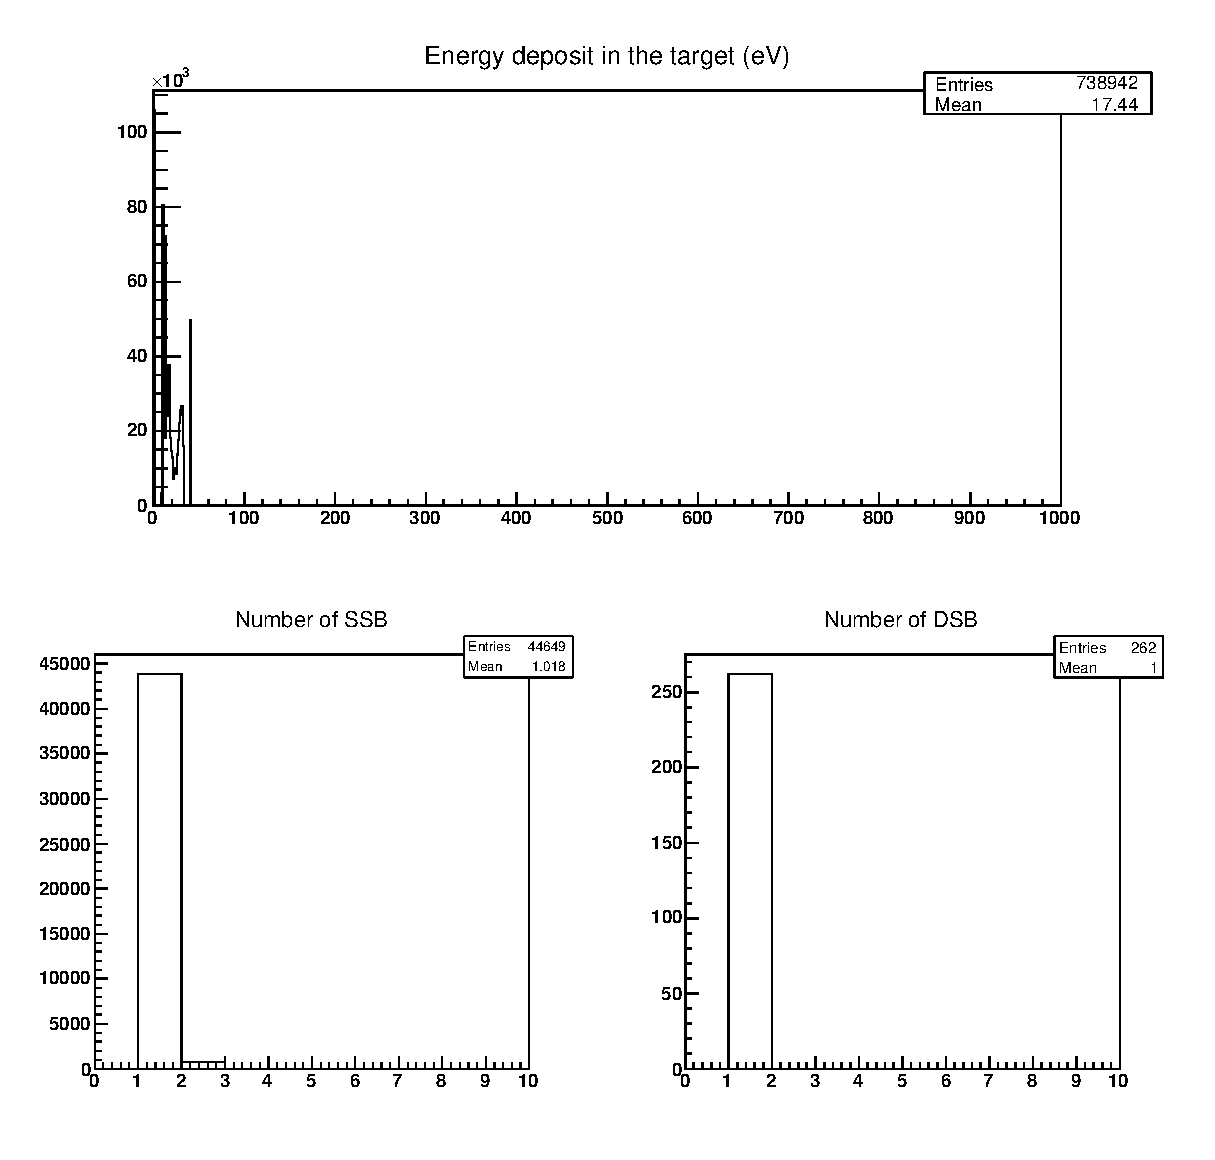
\includegraphics[width=.78\linewidth]{./Figures/1fzxe40ev.eps}
  \caption{40 eV}
  \label{fig:sube1}
\end{subfigure}%
\begin{subfigure}{.5\textwidth}
  \centering
  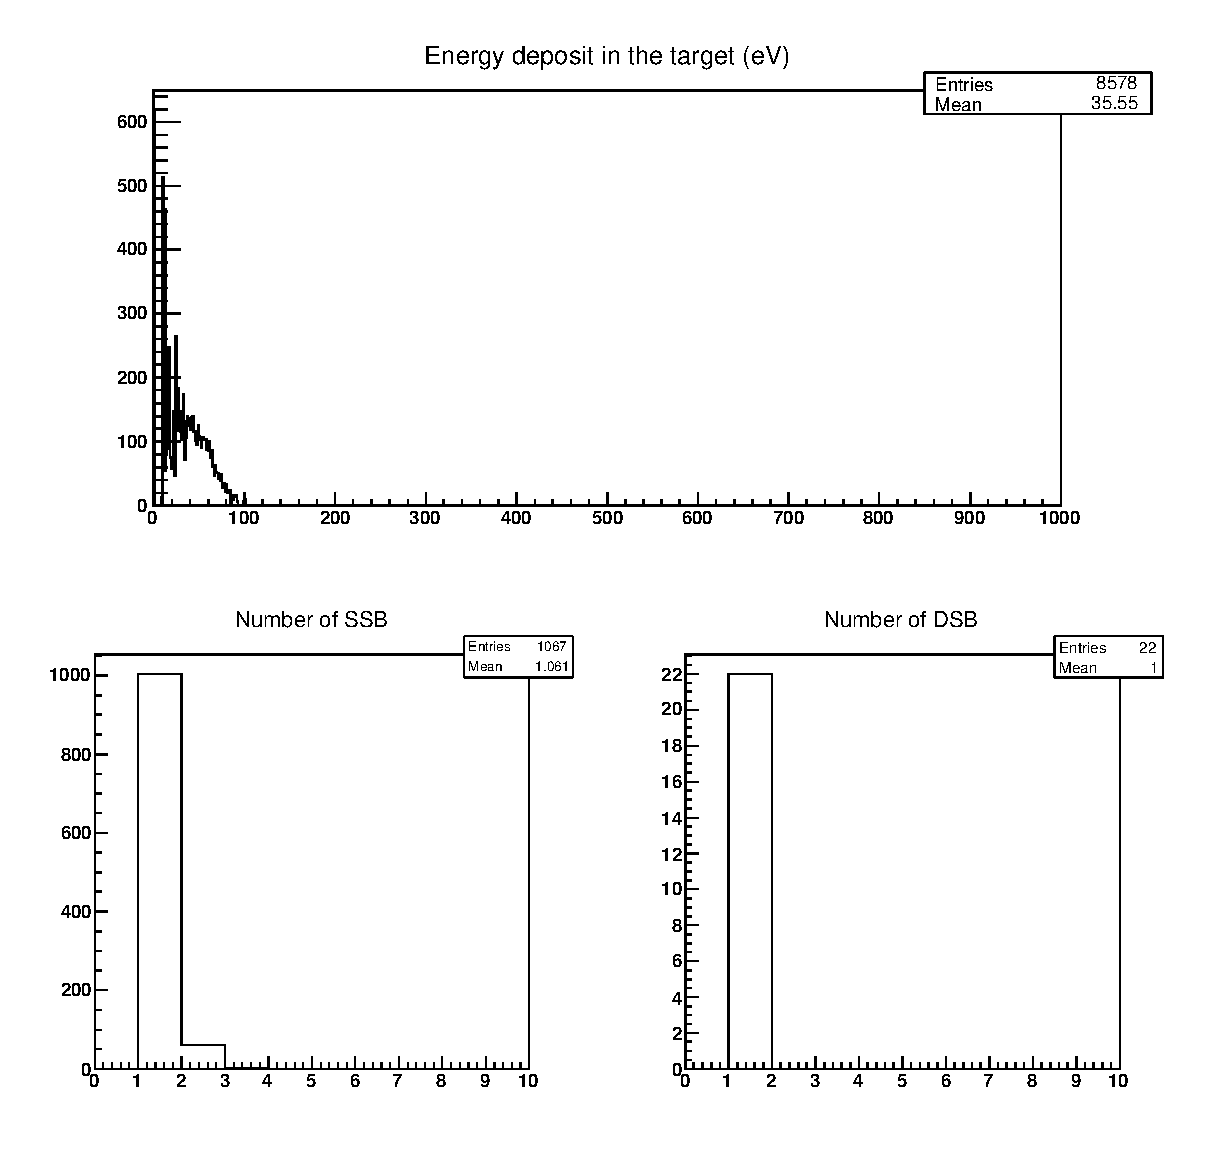
\includegraphics[width=.78\linewidth]{./Figures/1fzxe100ev.eps}
  \caption{100 eV}
  \label{fig:sube2}
\end{subfigure}
\begin{subfigure}{.5\textwidth}
  \centering
  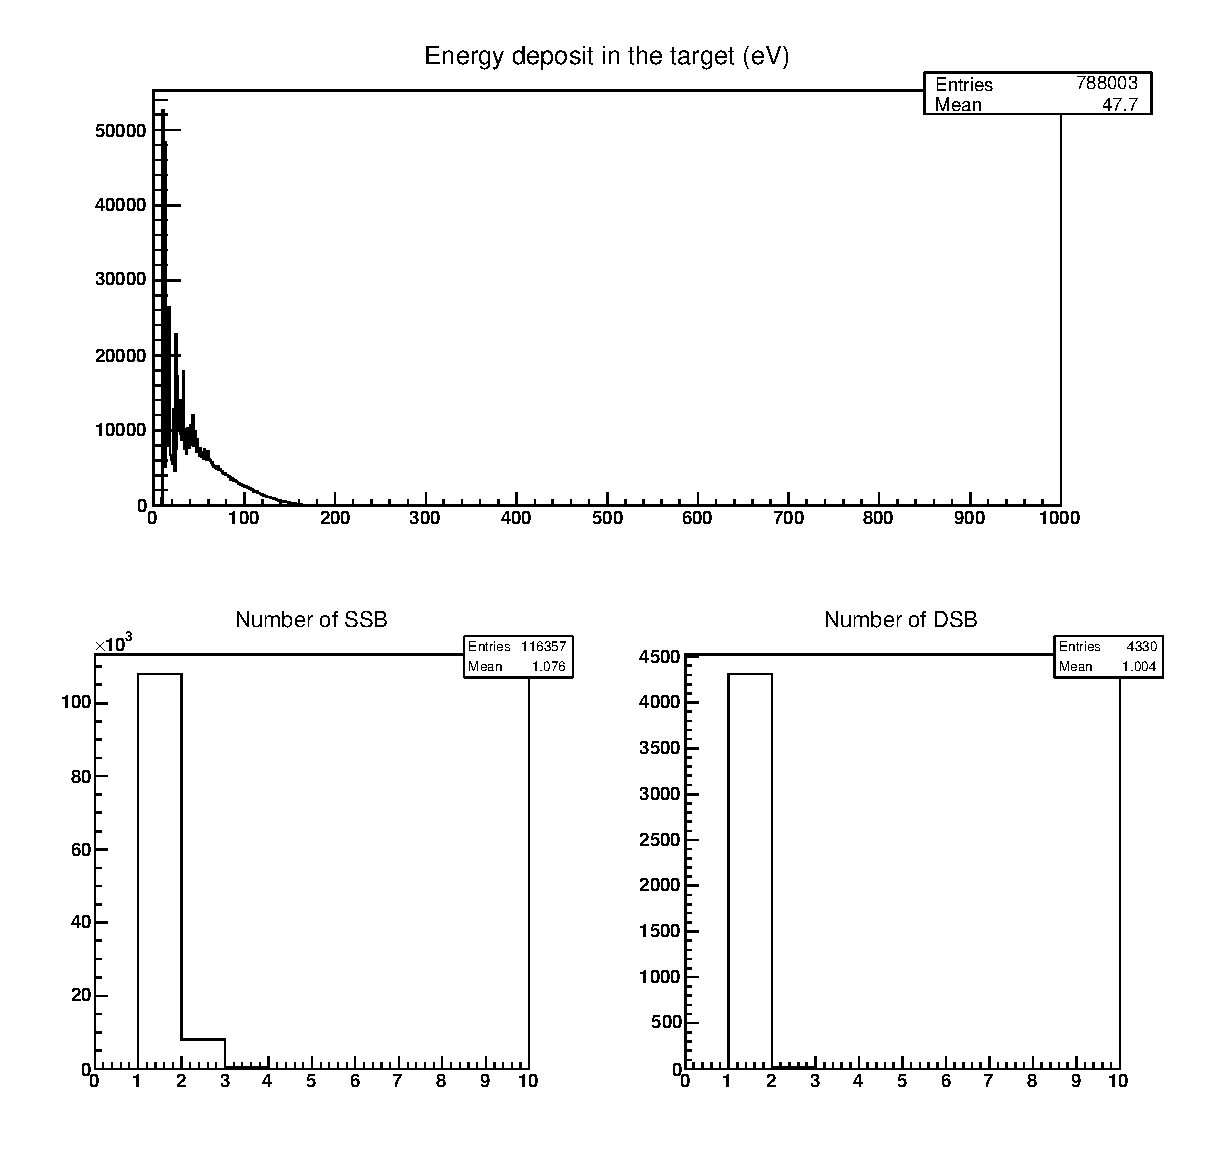
\includegraphics[width=.78\linewidth]{./Figures/1fzxe200ev.eps}
  \caption{200 eV}
  \label{fig:sube3}
\end{subfigure}%
\begin{subfigure}{.5\textwidth}
  \centering
  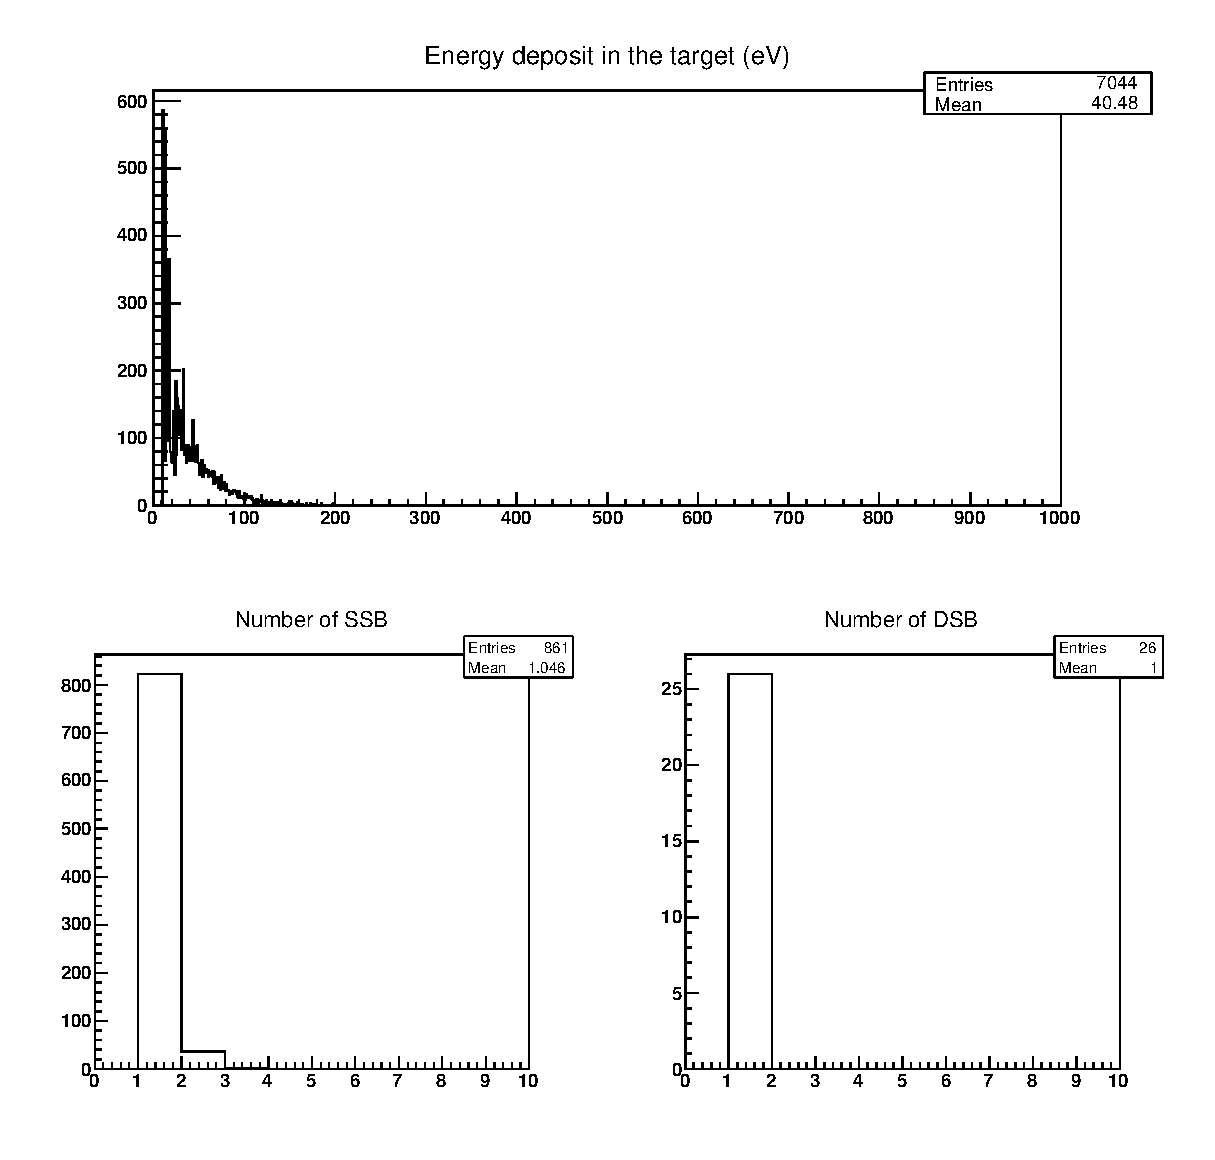
\includegraphics[width=.78\linewidth]{./Figures/1fzxe400ev.eps}
  \caption{400 eV}
  \label{fig:sube4}
\end{subfigure}
\begin{subfigure}{.5\textwidth}
  \centering
  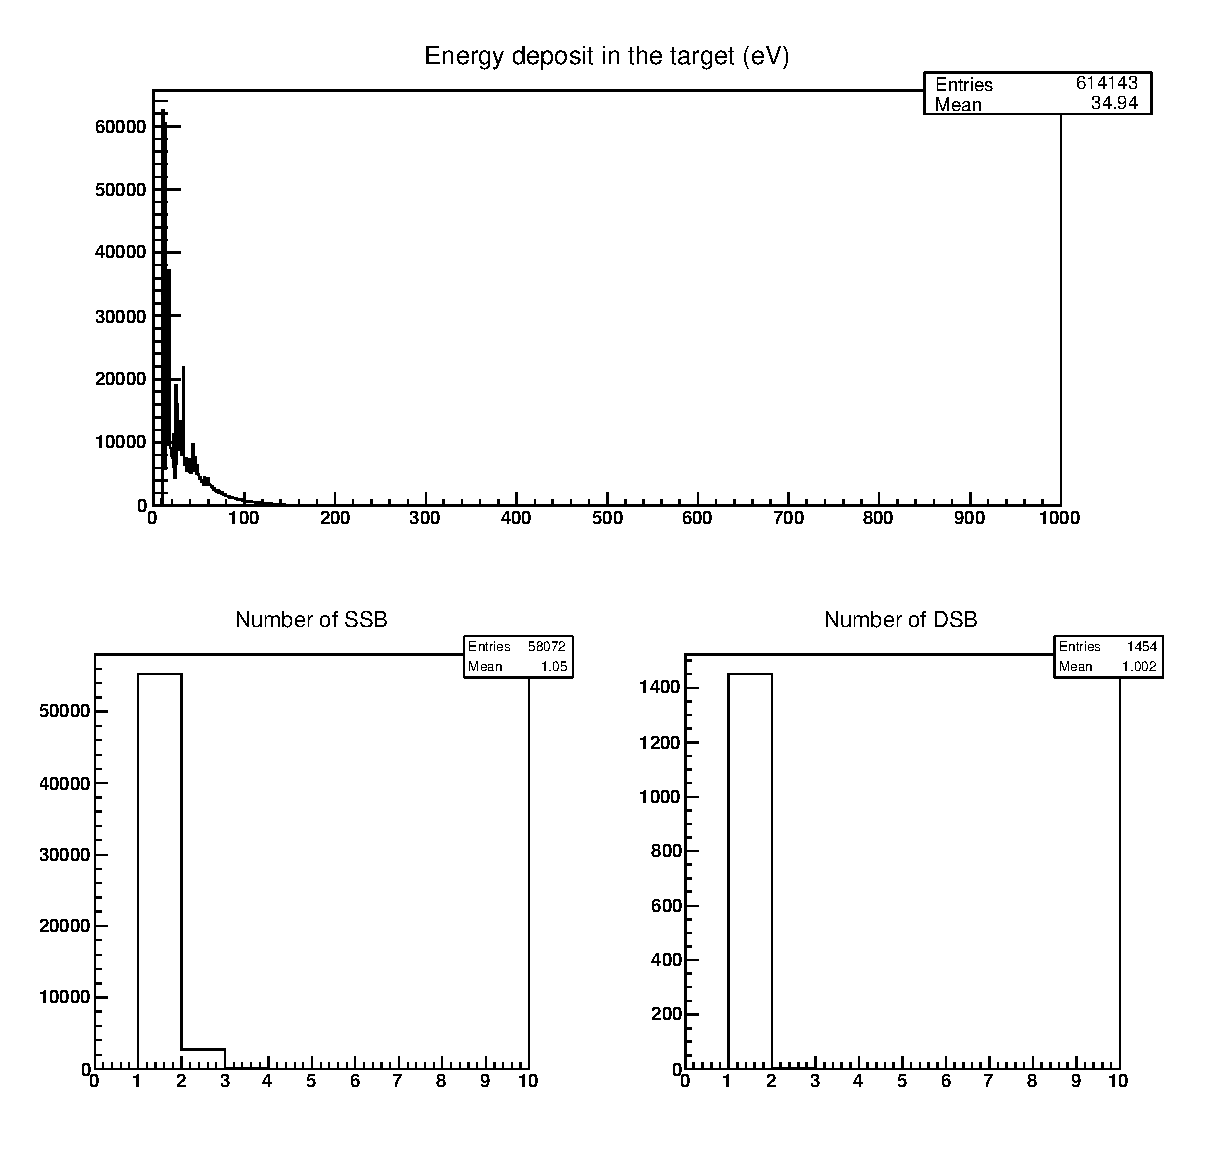
\includegraphics[width=.78\linewidth]{./Figures/1fzxe600ev.eps}
  \caption{600 eV}
  \label{fig:sube5}
\end{subfigure}%
\begin{subfigure}{.5\textwidth}
  \centering
  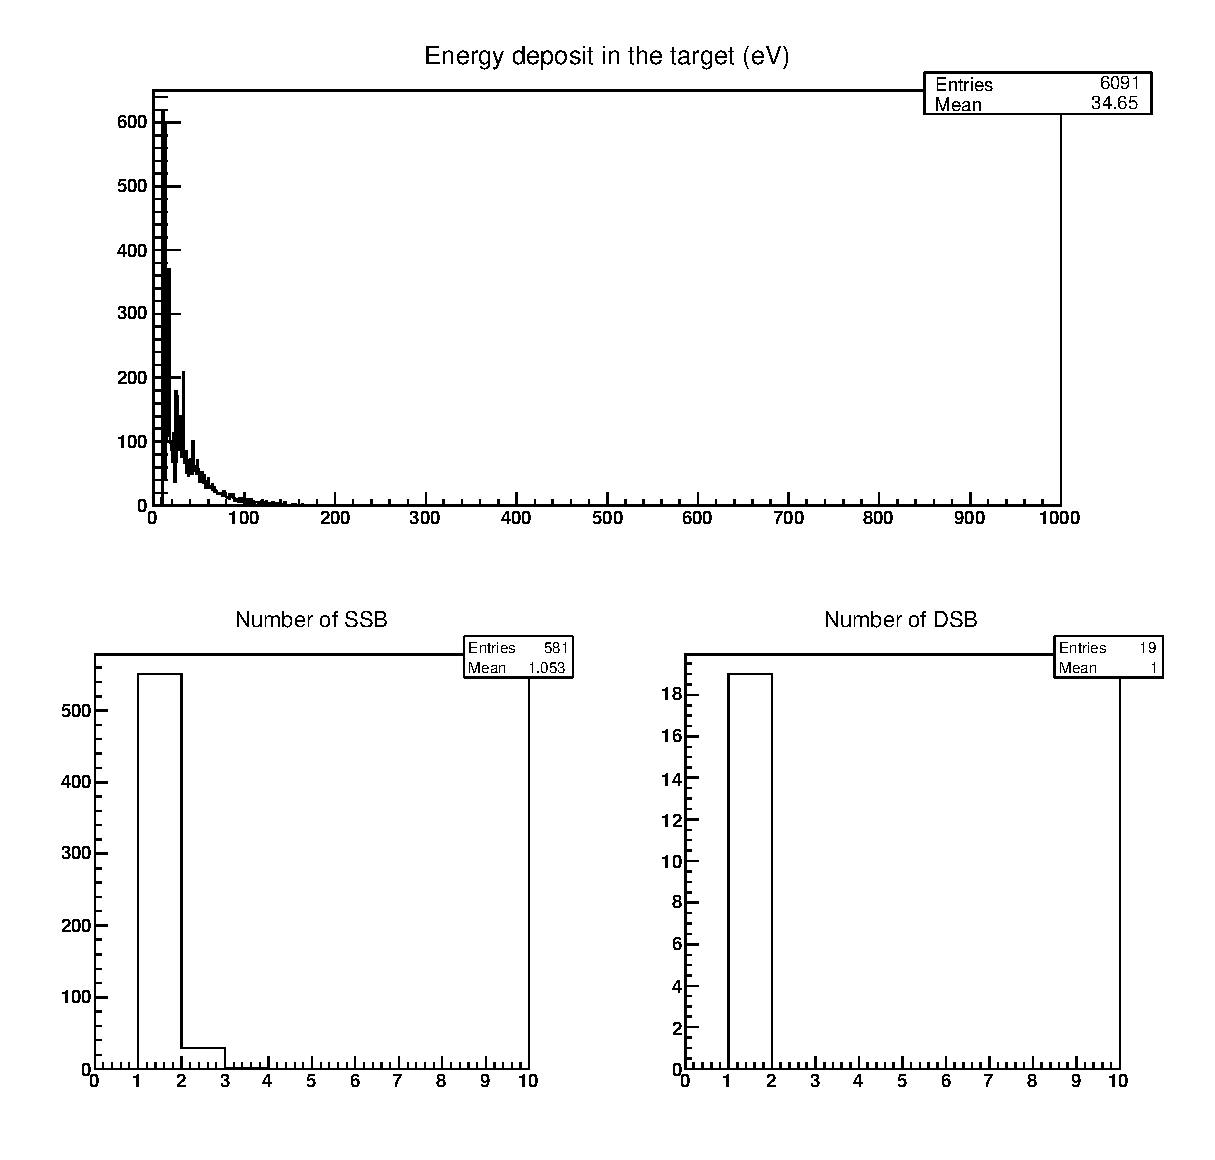
\includegraphics[width=.78\linewidth]{./Figures/1fzxe800ev.eps}
  \caption{800 eV}
  \label{fig:sube6}
\end{subfigure}
\begin{subfigure}{.5\textwidth}
  \centering
  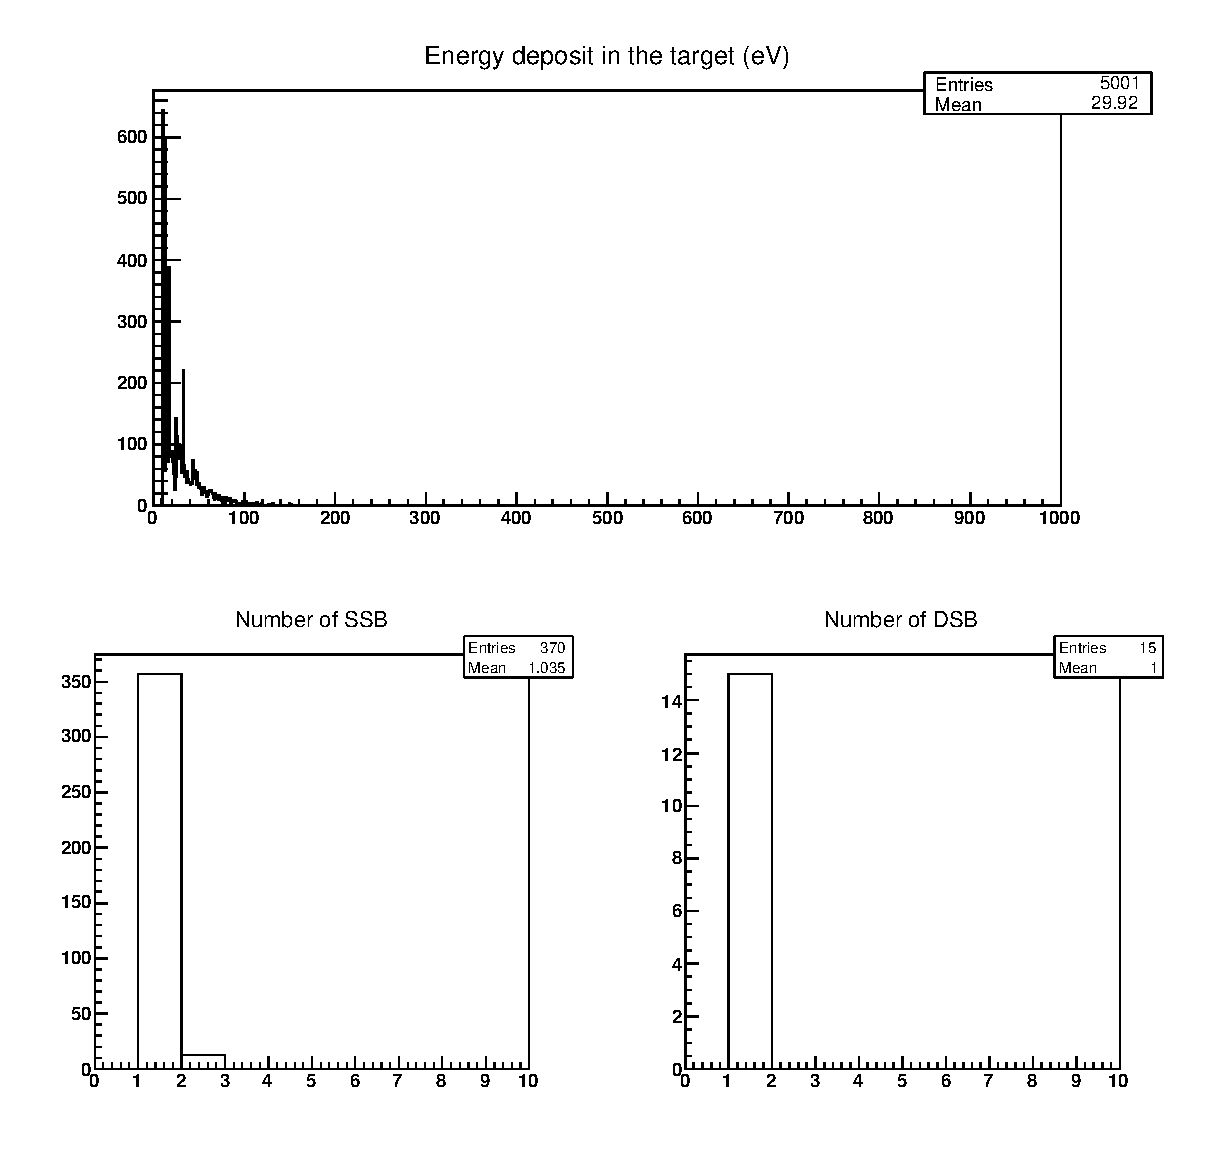
\includegraphics[width=.78\linewidth]{./Figures/1fzxe1kev.eps}
  \caption{1 keV}
  \label{fig:sube7}
\end{subfigure}%
\begin{subfigure}{.5\textwidth}
  \centering
  \includegraphics[width=.78\linewidth]{./Figures/1fzxe20kev.eps}
  \caption{20 keV}
  \label{fig:sube8}
\end{subfigure}
\caption{Rompimientos simples y dobles para 1FZX ($e-$)}
\label{fig:e2}
\end{figure}




\begin{figure}
\centering
\begin{subfigure}{.5\textwidth}
  \centering
  \includegraphics[width=.78\linewidth]{./Figures/1fzxp200ev.eps}
  \caption{200 eV}
  \label{fig:subi1}
\end{subfigure}%
\begin{subfigure}{.5\textwidth}
  \centering
  \includegraphics[width=.78\linewidth]{./Figures/1fzxp400ev.eps}
  \caption{400 eV}
  \label{fig:subi2}
\end{subfigure}
\begin{subfigure}{.5\textwidth}
  \centering
  \includegraphics[width=.78\linewidth]{./Figures/1fzxp600ev.eps}
  \caption{600 eV}
  \label{fig:subi3}
\end{subfigure}%
\begin{subfigure}{.5\textwidth}
  \centering
  \includegraphics[width=.78\linewidth]{./Figures/1fzxp800ev.eps}
  \caption{800 eV}
  \label{fig:subi4}
\end{subfigure}
\begin{subfigure}{.5\textwidth}
  \centering
  \includegraphics[width=.78\linewidth]{./Figures/1fzxp1kev.eps}
  \caption{1 keV}
  \label{fig:subi5}
\end{subfigure}%
\begin{subfigure}{.5\textwidth}
  \centering
  \includegraphics[width=.78\linewidth]{./Figures/1fzxp200kev.eps}
  \caption{200 keV}
  \label{fig:subi6}
\end{subfigure}
\begin{subfigure}{.5\textwidth}
  \centering
  \includegraphics[width=.78\linewidth]{./Figures/1fzxp400kev.eps}
  \caption{400 keV}
  \label{fig:subi7}
\end{subfigure}%
\begin{subfigure}{.5\textwidth}
  \centering
  \includegraphics[width=.78\linewidth]{./Figures/1fzxp600kev.eps}
  \caption{600 keV}
  \label{fig:subi8}
\end{subfigure}
\caption{Rompimientos simples y dobles para 1FZX ($proton$)}
\label{fig:p2}
\end{figure}




\begin{figure}
\centering
\begin{subfigure}{.4\textwidth}
  \centering
  \includegraphics[width=.78\linewidth]{./Figures/baresi.png}
  \caption{Baricentro residuos }
  \label{fig:sub11}
\end{subfigure}%
\begin{subfigure}{.4\textwidth}
  \centering
  \includegraphics[width=.78\linewidth]{./Figures/baresi.png}
  \caption{Centros de masa residuos}
  \label{fig:sub22}
\end{subfigure}
\begin{subfigure}{.4\textwidth}
  \centering
  \includegraphics[width=.78\linewidth]{./Figures/bavdw.png}
  \caption{Baricentro VDW}
  \label{fig:sub33}
\end{subfigure}%
\begin{subfigure}{.4\textwidth}
  \centering
  \includegraphics[width=.78\linewidth]{./Figures/bavdw.png}
  \caption{Centros de masa VDW}
  \label{fig:sub44}
\end{subfigure}
\begin{subfigure}{.4\textwidth}
  \centering
  \includegraphics[width=.78\linewidth]{./Figures/a.png}
  \caption{Baricentro esferas ligadas}
  \label{fig:sub55}
\end{subfigure}%
\begin{subfigure}{.4\textwidth}
  \centering
  \includegraphics[width=.78\linewidth]{./Figures/a.png}
  \caption{Centros de masa esferas ligadas}
  \label{fig:sub66}
\end{subfigure}
\caption[Comparación de centros de masa y baricentros en Geant4 1ZBB]{Comparación representación centros de masa y baricentros en Geant4 para 1ZBB}
\label{h}
\end{figure}




\begin{figure}
\centering
\begin{subfigure}{.4\textwidth}
  \centering
  \includegraphics[width=.78\linewidth]{./Figures/1fzxresid.png}
  \caption{Baricentros residuos}
  \label{fig:sub111}
\end{subfigure}%
\begin{subfigure}{.4\textwidth}
  \centering
  \includegraphics[width=.78\linewidth]{./Figures/1fzxresid.png}
  \caption{Centros de masa residuos}
  \label{fig:sub222}
\end{subfigure}
\begin{subfigure}{.4\textwidth}
  \centering
  \includegraphics[width=.78\linewidth]{./Figures/1fzxvdw.png}
  \caption{Baricentro VDW}
  \label{fig:sub333}
\end{subfigure}%
\begin{subfigure}{.4\textwidth}
  \centering
  \includegraphics[width=.78\linewidth]{./Figures/1fzxvdw.png}
  \caption{Centros de masa VDW}
  \label{fig:sub444}
\end{subfigure}
\begin{subfigure}{.4\textwidth}
  \centering
  \includegraphics[width=.78\linewidth]{./Figures/1fzxba.png}
  \caption{Baricentro esferas ligadas}
  \label{fig:sub555}
\end{subfigure}%
\begin{subfigure}{.4\textwidth}
  \centering
  \includegraphics[width=.78\linewidth]{./Figures/1fzxba.png}
  \caption{Centros de masa esferas ligadas}
  \label{fig:sub666}
\end{subfigure}
\caption[Comparación de centros de masa y baricentros en Geant4 1FZX]{Comparación representación centros de masa y baricentros en Geant4 para 1FZX}
\label{hh}
\end{figure}




\begin{figure}[htbp]
    \centering
  \caption[Baricentros en $x$ vs centros de masa en $x$ para 1ZBB]{Baricentros en $x$ vs centros de masa en $x$ para 1ZBB}
    \label{fig:canx}
    \includegraphics[width=1\linewidth]{./Figures/can1.eps}
\end{figure}

\begin{figure}[htbp]
    \centering
    \includegraphics[width=1\linewidth]{./Figures/can2.eps}
    \caption[Baricentros en $y$ vs centros de masa en $y$ para 1ZBB]{Baricentros en $y$ vs centros de masa en $y$ para 1ZBB}
    \label{fig:cany}
\end{figure}

\begin{figure}[htbp]
    \centering
    \includegraphics[width=1\linewidth]{./Figures/can3.eps}
  \caption[Baricentros en $z$ vs centros de masa en $z$ para 1ZBB]{Baricentros en $z$ vs centros de masa en $z$ para 1ZBB}
    \label{fig:canz}
\end{figure}




\begin{figure}[htbp]
    \centering
    \includegraphics[width=1\linewidth]{./Figures/1fzx.eps}
  \caption[Baricentros en $x$ vs centros de masa en $x$ para 1FZX]{Baricentros en $x$ vs centros de masa en $x$ para 1FZX}
    \label{fig:cax}
\end{figure}

\begin{figure}[htbp]
    \centering
    \includegraphics[width=1\linewidth]{./Figures/1fzy.eps}
  \caption[Baricentros en $y$ vs centros de masa en $y$ para 1FZX]{Baricentros en $y$ vs centros de masa en $y$ para 1FZX}
    \label{fig:cay}
\end{figure}

\begin{figure}[htbp]
    \centering
    \includegraphics[width=1\linewidth]{./Figures/1fzz.eps}
  \caption[Baricentros en $z$ vs centros de masa en $z$ para 1FZX]{Baricentros en $z$ vs centros de masa en $z$ para 1FZX}
    \label{fig:caz}
\end{figure}


% SEC6
\clearpage
\section{Conclusiones}
\label{sec:res}
Se ha mostrado que pdb4dna es una aplicación bastante interesante de Geant4 la cual permite realizar cálculos de deposición de energía y conteos tanto de rompimientos simples como dobles de ciertas moléculas de ADN mediante un archivo pdb con ciertas condiciones, bien la aplicación puede ser extendida al uso de moléculas de ADN más complejas y también otros tipos de moléculas, a partir de la energía depositada se presenta la posibilidad de modificar el código de manera que sabiendo donde se deposita la energía y el filtro poder realizar una localización de los rompimientos simples y dobles en la molécula de ADN lo cual permitiría el uso de gromacs para estudiar la dinámica propia de está.\\
En otra instancia también se modifico Geant4 para que usara centros de masa en lugar de esferas ligadas basadas en baricentros, al realizar histogramas tanto de las esferas ligadas y los baricentros no se ve ninguna diferencia en la deposición de energía ni en los rompimientos simples como dobles bajo las mismas condiciones de eventos, partículas, y energía. Esto se podría deber a que el código no esta tomando correctamente los centros de masa nuevos o a que el valor de la magnitud de las masas no afecta de forma relevante las posiciones del centro de masa respecto a las de los baricentros, sin embargo de ser la segunda opción esto podría cambiar de forma relevante con moléculas mucho más complejas o grandes debido a que como se observo en los histogramas de las diferentes posiciones de centros de masa contra baricentros se observan cambios a simple vista en las posiciones lo que resultaría en un cambio de la deposición de energía y en consecuencia de los rompimientos y posterior dinámica estructural, lo anterior se hizo con el fin de proponer un modelo alterno diferente a las esferas ligadas en baricentros con el fin de que sea más acercado al modelo general de átomos y masa.


% SEC7
%\clearpage
\section{Conclusiones}
\label{sec:res}




%%%%%%%%%%%%%%%%%%%%%%%%%%%%%%%%%%%%%%%%%%%%%%%%%%%%%%%%%%%%%
%APPENDICES
%%%%%%%%%%%%%%%%%%%%%%%%%%%%%%%%%%%%%%%%%%%%%%%%%%%%%%%%%%%%%


\appendix
\renewcommand*{\thesection}{\Alph{section}}\textbf{}

% APPENDIX A
%\clearpage
%\section{Anexo}
%\label{ede1}
%
%\begin{figure}
%\centering
%\begin{subfigure}{.5\textwidth}
%  \centering
%  \includegraphics[width=.78\linewidth]{./Figures/e-100ev.eps}
%  \caption{100 eV}
%  \label{fig:subei1}
%\end{subfigure}%
%\begin{subfigure}{.5\textwidth}
%  \centering
%  \includegraphics[width=.78\linewidth]{./Figures/e-200ev.eps}
%  \caption{200 eV}
%  \label{fig:subei2}
%\end{subfigure}
%\begin{subfigure}{.5\textwidth}
%  \centering
%  \includegraphics[width=.78\linewidth]{./Figures/e-400ev.eps}
%  \caption{400 eV}
%  \label{fig:subei3}
%\end{subfigure}%
%\begin{subfigure}{.5\textwidth}
%  \centering
%  \includegraphics[width=.78\linewidth]{./Figures/e-600.eps}
%  \caption{600 eV}
%  \label{fig:subei4}
%\end{subfigure}
%\begin{subfigure}{.5\textwidth}
%  \centering
%  \includegraphics[width=.78\linewidth]{./Figures/e-800ev.eps}
%  \caption{800 eV}
%  \label{fig:subei5}
%\end{subfigure}%
%\begin{subfigure}{.5\textwidth}
%  \centering
%  \includegraphics[width=.78\linewidth]{./Figures/e1kev.eps}
%  \caption{1 keV}
%  \label{fig:subei6}
%\end{subfigure}
%\begin{subfigure}{.5\textwidth}
%  \centering
%  \includegraphics[width=.78\linewidth]{./Figures/e20kev.eps}
%  \caption{20 keV}
%  \label{fig:subei7}
%\end{subfigure}%
%\begin{subfigure}{.5\textwidth}
%  \centering
%  \includegraphics[width=.78\linewidth]{./Figures/e40kev.eps}
%  \caption{40 keV}
%  \label{fig:subei8}
%\end{subfigure}
%\caption{Rompimientos simples y dobles para 1ZBB ($e-$)}
%\label{fig:e}
%\end{figure}
%
%\clearpage
%\section{Anexo}
%\label{ede2}
%
%\begin{figure}
%\centering
%\begin{subfigure}{.5\textwidth}
%  \centering
%  \includegraphics[width=.78\linewidth]{./Figures/proton200eV.eps}
%  \caption{200 eV}
%  \label{fig:sub1}
%\end{subfigure}%
%\begin{subfigure}{.5\textwidth}
%  \centering
%  \includegraphics[width=.78\linewidth]{./Figures/proton400eV.eps}
%  \caption{400 eV}
%  \label{fig:sub2}
%\end{subfigure}
%\begin{subfigure}{.5\textwidth}
%  \centering
%  \includegraphics[width=.78\linewidth]{./Figures/proton600eV.eps}
%  \caption{600 eV}
%  \label{fig:sub3}
%\end{subfigure}%
%\begin{subfigure}{.5\textwidth}
%  \centering
%  \includegraphics[width=.78\linewidth]{./Figures/proton800eV.eps}
%  \caption{800 eV}
%  \label{fig:sub4}
%\end{subfigure}
%\begin{subfigure}{.5\textwidth}
%  \centering
%  \includegraphics[width=.78\linewidth]{./Figures/proton1kev.eps}
%  \caption{1 keV}
%  \label{fig:sub5}
%\end{subfigure}%
%\begin{subfigure}{.5\textwidth}
%  \centering
%  \includegraphics[width=.78\linewidth]{./Figures/proton200kev.eps%}
%  \caption{200 keV}
%  \label{fig:sub6}
%\end{subfigure}
%\begin{subfigure}{.5\textwidth}
%  \centering
%  \includegraphics[width=.78\linewidth]{./Figures/proton400kev.eps%}
%  \caption{400 keV}
%  \label{fig:sub7}
%\end{subfigure}%
%\begin{subfigure}{.5\textwidth}
%  \centering
%  \includegraphics[width=.78\linewidth]{./Figures/proton600kev.eps%}
%  \caption{600 keV}
%  \label{fig:sub8}
%\end{subfigure}
%\caption{Rompimientos simples y dobles para 1ZBB ($proton$)}
%\label{fig:p}
%\end{figure}
%
%\clearpage
%\section{Anexo}
%\label{ede3}
%
%
%
%\begin{figure}
%\centering
%\begin{subfigure}{.5\textwidth}
%  \centering
%  \includegraphics[width=.78\linewidth]{./Figures/040.eps}
%  \caption{40 eV}
%  \label{fig:sube1}
%\end{subfigure}%
%\begin{subfigure}{.5\textwidth}
%  \centering
%  \includegraphics[width=.78\linewidth]{./Figures/1.eps}
%  \caption{100 eV}
%  \label{fig:sube2}
%\end{subfigure}
%\begin{subfigure}{.5\textwidth}
%  \centering
%  \includegraphics[width=.78\linewidth]{./Figures/2.eps}
%  \caption{200 eV}
%  \label{fig:sube3}
%\end{subfigure}%
%\begin{subfigure}{.5\textwidth}
%  \centering
%  \includegraphics[width=.78\linewidth]{./Figures/3.eps}
%  \caption{400 eV}
%  \label{fig:sube4}
%\end{subfigure}
%\begin{subfigure}{.5\textwidth}
%  \centering
%  \includegraphics[width=.78\linewidth]{./Figures/4.eps}
%  \caption{600 eV}
%  \label{fig:sube5}
%\end{subfigure}%
%\begin{subfigure}{.5\textwidth}
%  \centering
%  \includegraphics[width=.78\linewidth]{./Figures/5.eps}
%  \caption{800 eV}
%  \label{fig:sube6}
%\end{subfigure}
%\begin{subfigure}{.5\textwidth}
%  \centering
%  \includegraphics[width=.78\linewidth]{./Figures/6.eps}
%  \caption{1 keV}
%  \label{fig:sube7}
%\end{subfigure}%
%\begin{subfigure}{.5\textwidth}
%  \centering
%  \includegraphics[width=.78\linewidth]{./Figures/7.eps}
%  \caption{20 keV}
%  \label{fig:sube8}
%\end{subfigure}
%\caption{Rompimientos simples y dobles para 1FZX ($e-$)}
%\label{fig:e2}
%\end{figure}
%
%
%\clearpage
%\section{Anexo}
%\label{ede4}
%
%
%\begin{figure}
%\centering
%\begin{subfigure}{.5\textwidth}
%  \centering
%  \includegraphics[width=.78\linewidth]{./Figures/11.eps}
%  \caption{200 eV}
%  \label{fig:subi1}
%\end{subfigure}%
%\begin{subfigure}{.5\textwidth}
%  \centering
%  \includegraphics[width=.78\linewidth]{./Figures/22.eps}
%  \caption{400 eV}
%  \label{fig:subi2}
%\end{subfigure}
%\begin{subfigure}{.5\textwidth}
%  \centering
%  \includegraphics[width=.78\linewidth]{./Figures/33.eps}
%  \caption{600 eV}
%  \label{fig:subi3}
%\end{subfigure}%
%\begin{subfigure}{.5\textwidth}
%  \centering
%  \includegraphics[width=.78\linewidth]{./Figures/44.eps}
%  \caption{800 eV}
%  \label{fig:subi4}
%\end{subfigure}
%\begin{subfigure}{.5\textwidth}
%  \centering
%  \includegraphics[width=.78\linewidth]{./Figures/55.eps}
%  \caption{1 keV}
%  \label{fig:subi5}
%\end{subfigure}%
%\begin{subfigure}{.5\textwidth}
%  \centering
%  \includegraphics[width=.78\linewidth]{./Figures/66.eps}
%  \caption{200 keV}
%  \label{fig:subi6}
%\end{subfigure}
%\begin{subfigure}{.5\textwidth}
%  \centering
%  \includegraphics[width=.78\linewidth]{./Figures/77.eps}
%  \caption{400 keV}
%  \label{fig:subi7}
%\end{subfigure}%
%\begin{subfigure}{.5\textwidth}
%  \centering
%  \includegraphics[width=.78\linewidth]{./Figures/88.eps}
%  \caption{600 keV}
%  \label{fig:subi8}
%\end{subfigure}
%\caption{Rompimientos simples y dobles para 1FZX ($proton$)}
%\label{fig:p2}
%\end{figure}
%
%
\clearpage
\section{Anexo}
\label{app:M}
\lstset {language=C++}
\begin{lstlisting}
      double TotalMass = 0.0;
      double TotalMassPhosResSeq1 = 0.0;
      double TotalMassSugResSeq1 = 0.0;
      double TotalMassBaseResSeq1 = 0.0;
      double TotalMassPhosResSeq2 = 0.0;
      double TotalMassSugResSeq2 = 0.0;
      double TotalMassBaseResSeq2 = 0.0;


      for(int i = 0; i < residueListTemp->fNbAtom; i++)
      {
	//EM
      	//////////////////////////////////////
	// Set Mass expressed in u
        double ElementMass = 0.0;
        if(AtomTemp->fElement == "H") ElementMass = 1.00784;
	else if(AtomTemp->fElement == "C") ElementMass = 12.0107;
        else if(AtomTemp->fElement == "N") ElementMass = 14.0067;
        else if(AtomTemp->fElement == "O") ElementMass = 15.999;
        else if(AtomTemp->fElement == "P") ElementMass = 30.973762;
        else if(AtomTemp->fElement == "S") ElementMass = 32.065;
        else
	  {
          G4cerr << "Element not recognized : " << AtomTemp->fElement << G4endl;
          G4cerr << "Stop now" << G4endl;
          exit(1);
        }
\end{lstlisting}

\clearpage
\section{Anexo}
\label{app:CM}
\lstset {language=C++}
\begin{lstlisting}
//Center of mass calculation
else if( OptCalc == 2 )
  {
    baryX += ElementMass * (AtomTemp->fX);
    baryY += ElementMass * (AtomTemp->fY);
    baryZ += ElementMass * (AtomTemp->fZ);
    TotalMass += ElementMass;

    if(residueListTemp->fResSeq == 1)
      {
  if(i == 0)
    {
      baryPhosX += ElementMass * (AtomTemp->fX);
      baryPhosY += ElementMass * (AtomTemp->fY);
      baryPhosZ += ElementMass * (AtomTemp->fZ);
      TotalMassPhosResSeq1 += ElementMass;
    }
  else if(i < 8)
    {
      barySugX += ElementMass * (AtomTemp->fX);
      barySugY += ElementMass * (AtomTemp->fY);
      barySugZ += ElementMass * (AtomTemp->fZ);
      TotalMassSugResSeq1 += ElementMass;
    }
  else
    {
      //hydrogen are placed at the end of the residue in a PDB file
      //We don't want them for this calculation
      if(AtomTemp->fElement != "H")
        {
    baryBaseX += ElementMass * (AtomTemp->fX);
    baryBaseY += ElementMass * (AtomTemp->fY);
    baryBaseZ += ElementMass * (AtomTemp->fZ);
    TotalMassBaseResSeq1 += ElementMass;
        }
    }
      } //// if(residueListTemp->fResSeq == 1)........
    else  //if(residueListTemp->fResSeq != 1)
      {
  if(i < 4)
    {
      baryPhosX += ElementMass * (AtomTemp->fX);
      baryPhosY += ElementMass * (AtomTemp->fY);
      baryPhosZ += ElementMass * (AtomTemp->fZ);
      TotalMassPhosResSeq2 += ElementMass;
    }
  else if(i < 11)
    {
      barySugX += ElementMass * (AtomTemp->fX);
      barySugY += ElementMass * (AtomTemp->fY);
      barySugZ += ElementMass * (AtomTemp->fZ);
      TotalMassSugResSeq2 += ElementMass;
    }
  else
    {
      //hydrogen are placed at the end of the residue in a PDB file
      //We don't want them for this calculation
      if(AtomTemp->fElement != "H")
        { // break;
    baryBaseX += ElementMass * (AtomTemp->fX);
    baryBaseY += ElementMass * (AtomTemp->fY);
    baryBaseZ += ElementMass * (AtomTemp->fZ);
    TotalMassBaseResSeq2 += ElementMass;
        }
    }
      } // //if(residueListTemp->fResSeq != 1).......
  } //else if( OptCalc == 2 ).....
//Neither OpcCalc=1 nor OptCalc=2
else
  G4cerr << "Something is fishy!! : "  << G4endl;
AtomTemp = AtomTemp->GetNext();
    } //end of for (  i=0 ; i < residueListTemp->nbAtom ; i++)
\end{lstlisting}






%%%%%%%%%%%%%%%%%%%%%%%%%%%%%%%%%%%%%%%%%%%%%%%%%%%%%%%%%%%%%
%BIBLIOGRAPHY
%%%%%%%%%%%%%%%%%%%%%%%%%%%%%%%%%%%%%%%%%%%%%%%%%%%%%%%%%%%%%

\clearpage
\renewcommand*{\thesection}{}\textbf{}

%\bibliographystyle{apacite}
%\bibliography{Bibliography.bib}

\bibliography{Bibliography}

\end{document}
